% 서울대학교 컴퓨터공학부 석사ㅡ 박사 학위논문
% LaTeX 양식 샘플
\RequirePackage{fix-cm} % documentclass 이전에 넣는다.
% oneside : 단면 인쇄용
% twoside : 양면 인쇄용
% ko : 국문 논문 작성
% master : 석사
% phd : 박사
% openright : 챕터가 홀수쪽에서 시작
\documentclass[oneside,phd]{snuthesis}

%%%%%%%%%%%%%%%%%%%%%%%%%%%%%%%%%%%%%%%%%%%%%%%%%%%%%%%%%%%%%%%%%%%%%%%%%%%%%%
%%
%% Author: zeta709 (zeta709@gmail.com)
%% Releasedate: 2017/07/20
%%
%% 목차 양식을 변경하는 코드
%% * subfigure (subfig) package 사용 여부에 따라
%%   tocloft의 옵션을 다르게 지정해야 한다.
%% * Chapter 번호가 두 자리 수를 넘어가는 경우 다음과 같이
%%   필요한 만큼 "9"를 추가하면 된다.
%%   \settowidth{\mytmplen}{\bfseries\cftchappresnum9\cftchapaftersnum}
%%   아니면 \cftchapnumwidth를 직접 적당히 고치면 된다.
%%%%%%%%%%%%%%%%%%%%%%%%%%%%%%%%%%%%%%%%%%%%%%%%%%%%%%%%%%%%%%%%%%%%%%%%%%%%%%
%\usepackage[titles,subfigure]{tocloft} % when you use subfigure package
\usepackage[titles]{tocloft} % when you don't use subfigure package
\makeatletter
\if@snu@ko
	\renewcommand\cftchappresnum{제~}
	\renewcommand\cftchapaftersnum{~장}
	\renewcommand\cftfigpresnum{그림~}
	\renewcommand\cfttabpresnum{표~}
\else
	\renewcommand\cftchappresnum{Chapter~}
	\renewcommand\cftfigpresnum{Figure~}
	\renewcommand\cfttabpresnum{Table~}
\fi
\makeatother
\newlength{\mytmplen}
\settowidth{\mytmplen}{\bfseries\cftchappresnum\cftchapaftersnum}
\addtolength{\cftchapnumwidth}{\mytmplen}
\settowidth{\mytmplen}{\bfseries\cftfigpresnum\cftfigaftersnum}
\addtolength{\cftfignumwidth}{\mytmplen}
\settowidth{\mytmplen}{\bfseries\cfttabpresnum\cfttabaftersnum}
\addtolength{\cfttabnumwidth}{\mytmplen}
\makeatletter
\g@addto@macro\appendix{%
	\addtocontents{toc}{%
		\settowidth{\mytmplen}{\bfseries\protect\cftchappresnum\protect\cftchapaftersnum}%
		\addtolength{\cftchapnumwidth}{-\mytmplen}%
		\protect\renewcommand{\protect\cftchappresnum}{\appendixname~}%
		\protect\renewcommand{\protect\cftchapaftersnum}{}%
		\settowidth{\mytmplen}{\bfseries\protect\cftchappresnum\protect\cftchapaftersnum}%
		\addtolength{\cftchapnumwidth}{\mytmplen}%
	}%
}
\makeatother
 % SNU toc style

%%%%%%%%%%%%%%%%%%%%%%%%%%%%%%%%%%%%%%%%
%% 다른 패키지 로드
%% http://faq.ktug.or.kr/faq/pdflatex%B0%FAlatex%B5%BF%BD%C3%BB%E7%BF%EB
%% 필요에 따라 직접 수정 필요
\ifpdf
	\input glyphtounicode\pdfgentounicode=1 %type 1 font사용시
	%\usepackage[pdftex,unicode]{hyperref} % delete me
	\usepackage[pdftex]{graphicx}
	%\usepackage[pdftex,svgnames]{xcolor}
\else
	%\usepackage[dvipdfmx,unicode]{hyperref} % delete me
	\usepackage[dvipdfmx]{graphicx}
	%\usepackage[dvipdfmx,svgnames]{xcolor}
\fi
%%%%%%%%%%%%%%%%%%%%%%%%%%%%%%%%%%%%%%%%

% \usepackage{graphicx,epsfig,wrapfig,url,xcolor,listings}

% TODO: additional packages
\usepackage{epsfig}
\usepackage{wrapfig}
\usepackage{graphicx}
\usepackage{xcolor}
\usepackage{url}
\usepackage{listings}
\usepackage{footnote}
\usepackage{algorithmic}
\usepackage{mathtools}
\usepackage{caption}
\usepackage{booktabs}
\usepackage{makecell}
\usepackage{soul}
\usepackage{diagbox}
\usepackage{tabularx}
\usepackage[hidelinks]{hyperref}
\usepackage{float}
\usepackage{subcaption}

\newcommand{\hwkim}[1]{{\color{teal}{\small\bf\sf [HW: #1]}}}
\newcommand{\new}[1]{#1}

%% \title : 22pt로 나오는 큰 제목
%% \title* : 16pt로 나오는 작은 제목
\title{Your Ph.D. Thesis \\ Title}
\title*{우리말 제목}

\academicko{공학}
\schoolen{COLLEGE OF ENGINEERING}
% 2013학번까지 전기.컴퓨터공학부
%\departmenten{DEPARTMENT OF ELECTRICAL ENGINEERING & COMPUTER SCIENCE}
%\departmentko{전기$\cdotp$컴퓨터 공학부}
% 2014학번부터 컴퓨터공학부
\departmenten{DEPARTMENT OF COMPUTER SCIENCE \& ENGINEERING}
\departmentko{컴퓨터공학부}

%% 저자 이름 Author's(Your) name
\author{Your name}
\author*{네~이~름} % Insert space for Hangul name.

%% 학번 Student number
%\studentnumber{XXXX-XXXXX}

%% 지도교수님 성함 Advisor's name
%% (?) Use Korean name for Korean professor.
\advisor{Your advisor's name}
\advisor*{교~수~님} % Insert space for Hangul name.

%% 학위 수여일 Graduation date
%% 표지에 적히는 날짜.
%% 여름졸업이면 8월, 겨울졸업이면 2월
%\graddate{2022~년~2~월}
\graddate{August 2023}

%% 논문 제출일 Submission date
%% (?) Use Korean date format.
%% 컴공 논문 제본 요령: "논문심사계획"상의 심사용 논문제출기한이 속하는 연,월.
%% 최초 심사용 논문을 제출하는 날이므로, 일반적으로 심사 학기 시작월.
\submissiondate{2023~년~02~월}

%% 논문 인준일 Approval date
%% (?) Use Korean date format.
%% 컴공 논문 제본 요령: "논문심사계획"상의 논문종심일이 속하는 연,월.
%% 실제 인준지에 서명받은 날로 적으면 됨.
\approvaldate{2023~년~05~월}

%% Note: 인준지의 교수님 성함은
%% 컴퓨터로 출력하지 않고, 교수님께서
%% 자필로 쓰시기도 합니다.
%% Committee members' names
%% 위원장, 교수님, 나머지 심사위원들 순으로 이름을 적습니다.
\committeemembers%
{위~원~장}%
{지~도~교~수~님}%
{교~수~님}%
{교~수~님}%
{교~수~님}
%% Length of underline
%\setlength{\committeenameunderlinelength}{7cm}
\usepackage{pdfpages}

\begin{document}

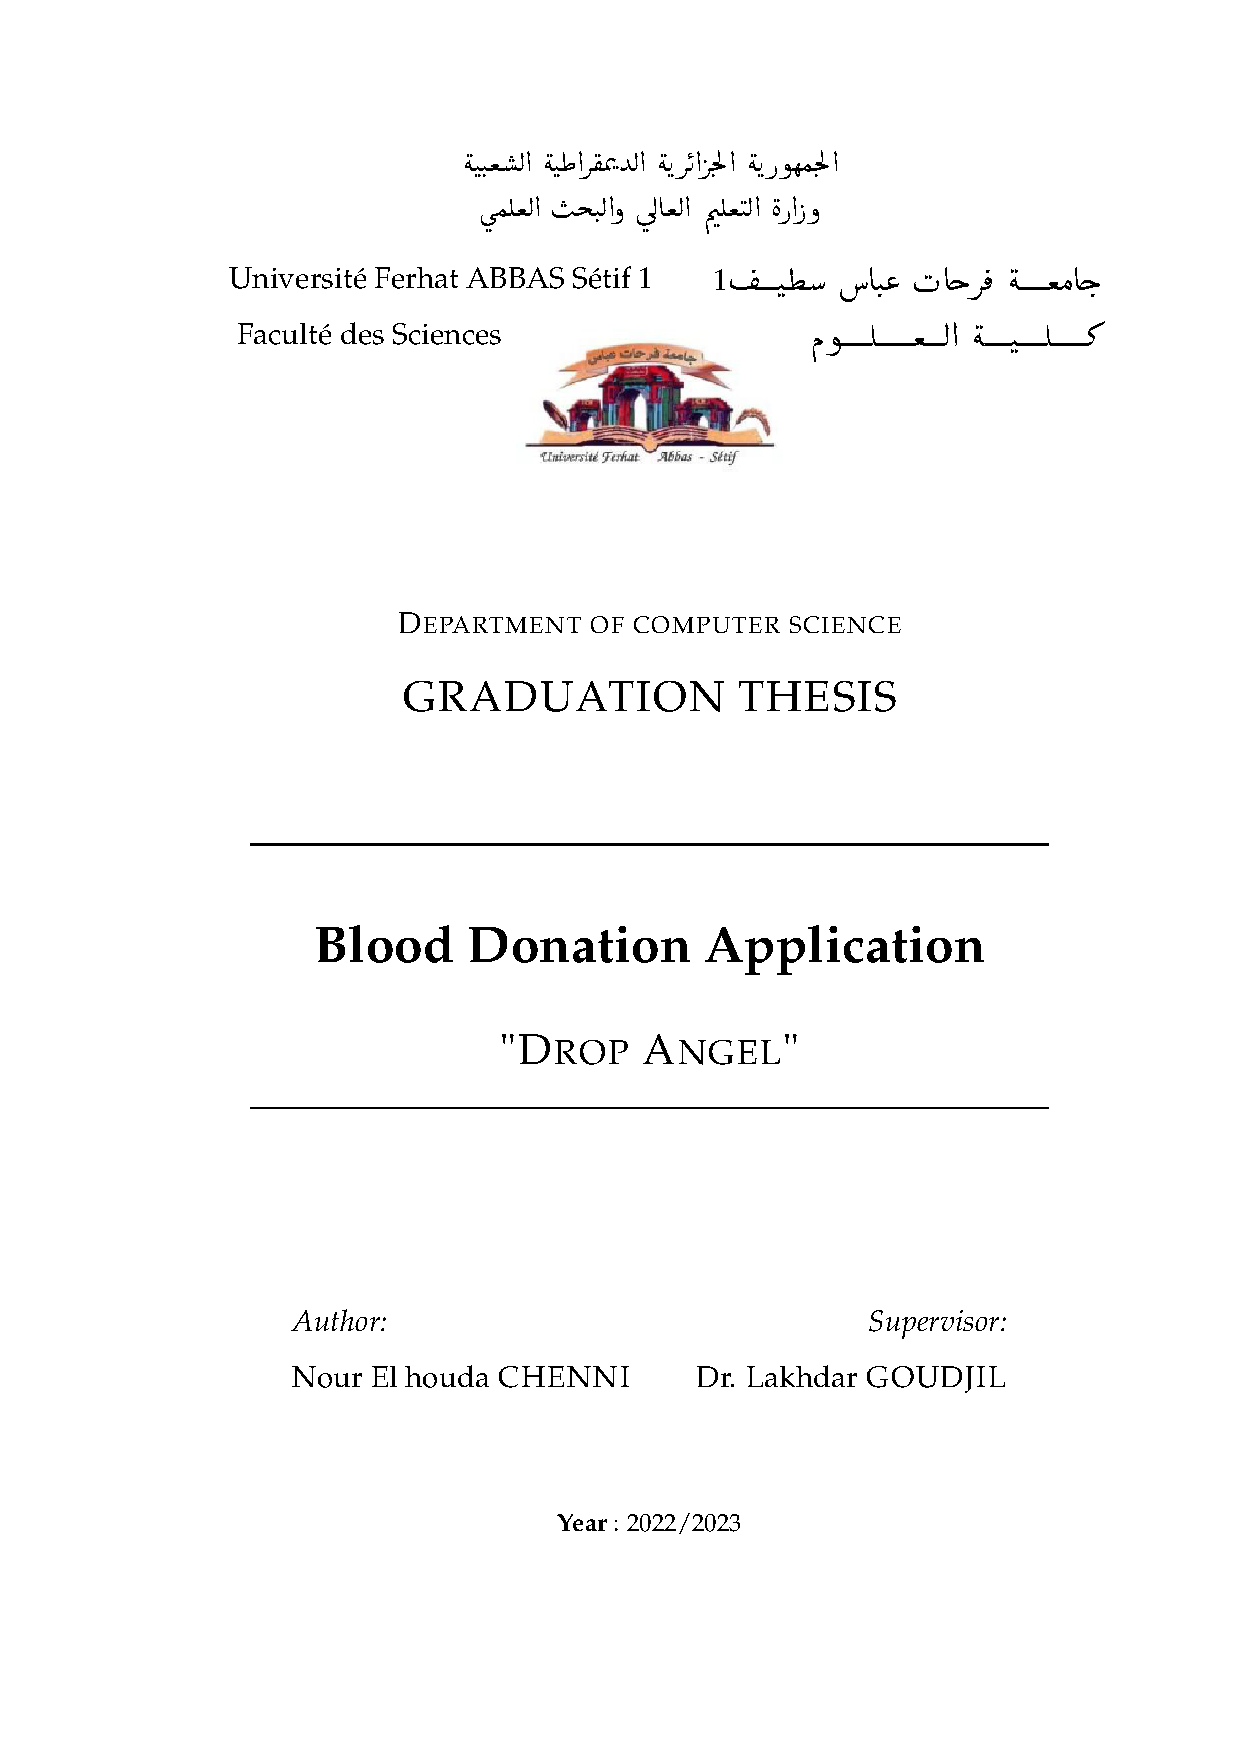
\includepdf[page={1}]{firstpage}
%\begin{titlepage}
\begin{center}


\vspace*{-0.1\textheight}

%\textbf{}


\<    الجمهورية الجزائرية الديمقراطية الشعبية >\\

\<  وزارة التعليم العالي والبحث العلمي >
\\[1cm]


\begin{figure}[h]
    \centering
    
\includegraphics[width=0.3\linewidth]{univfrhat.PNG}
    
\end{figure}






\begin{minipage}[t]{0.6\textwidth}
\begin{flushleft} \large
\vspace*{-0.2\textheight}
\hspace*{-0.02\textheight}
{Université Ferhat ABBAS  Sétif 1}\\
\hspace*{-0.02\textheight}
{ Faculté des Sciences }
\end{flushleft}
\end{minipage}
\begin{minipage}[t]{0.3\textwidth}
\begin{flushright} \large
\vspace*{-0.225\textheight}  %0.04
\hspace*{-0.06\textheight}
{1\<جامعـــة فرحات عباس	سطيــف    >} \\
\hspace*{0.01\textheight}
{  \<    كــــلـــيـــة الــعــــلـــوم>        
}


\end{flushright}
\end{minipage}\\%[1cm]


\begin{minipage}[t]{0.6\textwidth}
\begin{flushleft} \large
\vspace*{-0.05\textheight}
\hspace*{-0.12\textheight}
{Département : }
{Informatique}
\end{flushleft}
\end{minipage}

\thesistitle{Blood Donation Application}

\supervisor{Dr. Lakhdar \textsc{GOUDJIL}}

\author{Nour El houda \textsc{CHENNI}}

\department{\href{https://fsciences.univ-setif.dz/sites_departements/informatique}{Département d’Informatique}} % Your department's name and URL, this is used in the title page and abstract, print it elsewhere with \deptname
\group{{Fondements et ingénierie de l’information et de l’image}} % Your research group's name and URL, this is used in the title page, print it elsewhere with \groupname
\faculty{\href{https://fsciences.univ-setif.dz/main_page/home}{Faculté des Sciences}} % Your faculty's name and URL, this is used in the title page and abstract, print it elsewhere with \facname



{\scshape\LARGE MEMOIRE DE MASTER\par}%\vspace{1.5cm} % University name
%\textsc{\Large MEMOIRE DE MASTER}\\[0.5cm] % Thesis type

%DOMAINE : Informatique\\
%FILIERE :Informatique\\
%SPECIALITE : Fondement et Ingénierie de l’information et de l’image\\

\HRule \\[0.4cm] % Horizontal line
{\huge \bfseries \ttitle\par}\vspace{0.4cm} % Thesis title
\HRule \\[1.5cm] % Horizontal line
 
\begin{minipage}[t]{0.4\textwidth}
\begin{flushleft} \large
\emph{Présenté par:}\\
{\authorname} % Author name - remove the \href bracket to remove the link
\end{flushleft}
\end{minipage}
\begin{minipage}[t]{0.4\textwidth}
\begin{flushright} \large
\emph{Dirigé par:} \\
{\supname} % Supervisor name - remove the \href bracket to remove the link  
\end{flushright}
\end{minipage}\\[4cm]
 


\textbf{Promotion} : 2022/2023\\[4cm] % Date
%\includegraphics{Logo} % University/department logo - uncomment to place it
 
\vfill
\end{center}
\end{titlepage}



\pagenumbering{Roman}
  %\makefrontcover
 %\makefrontcover
% \makeapproval








% not final one...
\iffalse

\thispagestyle{empty}
\newpage
\mbox{}
\newpage

\makefrontcover
% 임시 제본이라 인준지가 필요없는 경우 아래줄을 지우세요.
\makeapproval

\fi

\cleardoublepage
%\pagenumbering{arabic}
% 초록 Abstract

% 이제 평소 논문 쓰시듯 쓰면 됩니다.


% \keyword{Deep Learning, Natural Language Processing, Open-domain
% Dialogue, Social Cognition, Social Commonsense}


%\begin{abstract}
 %   Hello, there! Attention is all you need to graduate %\cite{Vaswani:2017:NeurIPS}.
%\end{abstract}



   
\begin{abstract}
 %   Hello, there! Attention is all you need to graduate %\cite{Vaswani:2017:NeurIPS}.


At the end of our computer science degree program, we were tasked with completing a final year project, and we decided to develop a mobile application for blood donation. Our project aimed to provide a user-friendly platform for individuals to donate blood and connect with blood donation centers. The development of the blood donation app allowed us to learn about a new development platform and expand our knowledge and experience.

Our final year project consisted of three major chapters. In the first chapter, we conducted entrance to mobile applications in the medical field, followed by a conceptual study of our "Drop Angel" application in the second chapter. The third chapter focused on our work environment, including the installation of various development tools, as well as screenshots of the different interfaces in our application.



\end{abstract}
 





%\pagenumbering{Roman}
\acknowledgement


"All praises be to \textbf{Allah}, whom we depend for help and guidance."

First, I would like to express my sincere gratitude to my supervisor for his continuous support, patience, motivation. His guidance helped me in all the time of research and writing of this thesis. 

I am very thankful to many friends for their support, encouragement, helps,listening during this thesis as well as before it.

Last but not the least, I would like to mention the contribution of my family as the main source of strength in my life. I am grateful the unconditional support and affection of my parents.

This thesis would not have been possible without these people.


%\pagenumbering{Roman}


\tableofcontents
%\listoffigures
%\listoftables

\cleardoublepage




\pagenumbering{arabic}


\addcontentsline{toc}{chapter}{ Introduction}
\chapter*{Introduction}
The desire to benefit others at a cost to the self is the most commonly frequently mentioned reason for donating blood which is the most precious thing that anyone can give to any one in need ,and that can save millions of lives. Even though people do not donate blood regularly, there is a constant effort to balance the supply and demand of blood. 
As in Algeria, almost all Willayas facing the difficulty to beg for blood donors, recognized
by the Algerian donation centers. The problem is getting worse especially during the
festive and holiday seasons. Since there is a serious blood shortage in the blood bank, accident victims
who are in need of blood are not be able to be saved. A minimal participation from Algerian
citizens is recorded, even though blood donation activities are organized everywhere. This issue has created
the need to understand the population and associate factors that can increase their motivation
and willingness to be a blood donor,and that the aim of "Drop Angel" which is a mobile application 
 designed to connect blood donors with blood banks and hospitals in need of blood products , enhance the efficiency of the blood donation process and
to create awareness and encourage others to be a blood donors
This thesis is divided into 3 chapters\cite{uptodate}, with:
\newline


\begin{itemize}

\item \textbf {Chapter 1 (Mobile Applications in the Medical Field):}\newline
This chapter discusses the use of mobile apps in the medical field to support blood centers and blood donation


\item \textbf {Chapter 2 (Analysis and Design):}\newline
This section is devoted to the analysis and design of our application,using the UML method with the help of use case diagrams,diagrams of sequences and class diagrams.


\item \textbf {Chapter 3 (Implementation):} \newline
This part presents the realization and implementation of our application in which we illustrate the different parts of the application and the tools used to make it

\end{itemize}





\chapter{Mobile Applications in Medical Field}


\section{Introduction}
\label{sec:contribution}
The medical field is constantly evolving, and technology has played a critical role in facilitating and improving healthcare services. One such technology that has gained widespread popularity in recent years is mobile applications. In the field of blood donation, mobile apps have the potential to play a significant role in supporting blood centers and improving the efficiency of blood collection and distribution processes. This chapter explores the mobile applications, their use in the medical field to promote blood donation and their potential benefits,..

\section{Mobile Applications}
\label{sec:organization}
\subsection{Definition}

A mobile application, or mobile app, is a software application designed to run on mobile devices such as smartphones or tablets, providing a variety of functions and features such as social networking, gaming, productivity tools, and entertainment.

\subsection{Types of Mobile Applications}

\begin{itemize}
\item \textbf{Native apps:} These are built specifically for a particular mobile platform, such as iOS or Android, and are written in the programming languages supported by that platform.
\item \textbf{Web apps:} These are mobile-optimized websites that are accessed through a mobile device's web browser, and are not downloaded from an app store.
\item \textbf{Hybrid apps:} These are a combination of native and web apps, built using web technologies like HTML, CSS, and JavaScript, but packaged as native apps for distribution on app stores.
\item \textbf{Gaming apps:} These apps are designed for playing games on mobile devices, ranging from simple puzzles to complex multiplayer games.
\item \textbf{Social media apps:} These apps allow users to connect and communicate with others, such as Facebook, Twitter, Instagram, and LinkedIn.
\item \textbf{Lifestyle apps:} These apps are designed to help users with their daily routines and activities, such as fitness apps, diet trackers, and meditation apps.
\end{itemize}

\subsection{Operating Systems}
There are several mobile operating systems used in smartphones, including:

\begin{itemize}
\item \textbf{Android:}  Developed by Google, Android is the most widely used mobile operating system, used by many smartphone manufacturers such as Samsung, Huawei, and Xiaomi.
\item \textbf{IOS:} Developed by Apple, iOS is used exclusively on iPhones and iPads.
\item \textbf{BlackBerry OS:}  Developed by BlackBerry Limited, this operating system is used exclusively on BlackBerry smartphones.
\end{itemize}

\subsection{Benefits of Mobile Applications}
Mobile applications offer several advantages, including increased accessibility, personalization, improved user experience, offline access, increased engagement, increased efficiency, and new revenue streams. Mobile apps are designed to provide a seamless and intuitive user experience, with easy navigation and optimized features for the mobile platform

\subsection{Examples of Mobile Applications}

\subsubsection{Health Applications}

\begin{itemize}
\item \textbf{UpToDate} a clinical decision support app that provides evidence-based medical information on diagnosis, treatment, and management of various conditions. It requires a subscription for access.\cite{uptodate}
\item \textbf{Headspace} a meditation and mindfulness app that offers guided meditations and exercises to help users reduce stress, improve sleep, and increase focus.\cite{headspace}
\end{itemize}
\subsubsection{Blood donation Applications}
\begin{itemize}
\item \textbf{Blood Donor by Blood Bank of Delmarva:} an app that allows users to schedule blood donation appointments, view their donation history, and receive notifications about local blood drives. It also provides personalized health insights based on donation history. 
\item \textbf{Blood Donor Finder by Blood Bank Alliance:}  an app that allows users to locate nearby blood banks, view their inventory, and request blood donation. It also provides information on blood donation and health.\cite{bloodbankalliance}
\end{itemize}


%\input{02-background.tex}


\chapter{Analysis and Design}
\label{chp:paper01}
% vim: set ft=tex:

\section{Introduction}
In software development, there are several critical steps that must be followed in order to create a successful software application. Among these steps are the analysis and design phases. The analysis phase involves gathering requirements and understanding the needs of the users and stakeholders. This phase is crucial because it lays the foundation for the design phase, which involves creating a plan for how the software will be built and what it will do.



\section{Scope Statement}
A blood donation app is a mobile application designed to connect blood donors with blood banks and hospitals to facilitate blood donations. The app allows users to register as donors, search for nearby blood banks and hospitals in need of donations, schedule appointments, and track their donation history. The aim of the project is to increase access to blood donations and make the donation process more convenient for both donors and recipients.

\begin{itemize}
\item \textbf{Project Objective:} The objective of this project is to design and develop a mobile application that allows individuals to easily schedule appointments to donate blood in nearby blood banks and hospitals, and track their donation history.
\item \textbf{Project Deliverables: }The project will deliver a fully functional mobile application for Android devices. The application will include features such as user registration, appointment scheduling, donation tracking, and notifications for blood banks and hospitals in need of donations.
\item \textbf{Project Boundaries:} The project will include the development of the mobile application and any necessary server-side components. The project will not include the physical collection or transportation of blood.
\item \textbf{Project Constraints:} The project must be completed within a budget of 200000 DA and a timeframe of 2 months.
\item \textbf{Project Assumptions: } The project assumes that there is a need for a blood donation app, that potential users have access to smartphones and the internet, and that there are a sufficient number of blood banks and hospitals interested in using the app.
\item \textbf{Project Sub Functions:} 
\begin{itemize}
\item  User registration
\item  Profile management
\item Appointment scheduling
\item  Donation tracking (history of donations)
\item  Notifications for blood banks and hospitals
\end{itemize}
\item \textbf{Actors(Stakeholders):} 
\begin{itemize}
\item \textbf{Donor:}  the application allows the donor to:
\begin{itemize}
\item  Authantificate 
\item  Make donation
\item See content about blood donation process
\item  Check the tests result
\item  Check the history of donations
\item  Check his profile
\item  Edit / delete profile
\item  Receive notifications
\end{itemize}
\item \textbf{Admin:}  The admin is able to use the application to:
\begin{itemize}
\item  Authenticate 
\item  See content about blood donation process
\item Send test result
\item  Send notifications
\end{itemize}
\item \textbf{Guest:}  guests are able to:
\begin{itemize}
\item  Register 
\item  See content about blood donation process
\end{itemize}
\end{itemize}
\end{itemize}


\section{Unified Modeling Language(UML)}


\subsection{Definition}
Unified Modeling Language (UML) is a standardized visual language used in software engineering to document, design, and analyze software systems. It provides a common language for understanding and describing the different aspects of a software system through diagrams and models.

\begin{figure}[H]
    \centering
    
\includegraphics[width=0.5\textwidth]{images/UML_logo.svg.png}
    \caption{UML logo}
    \label{fig:figure4}
\end{figure}
\subsection{UML Advantages}

\begin{itemize}
\item  Helps in communication
\item   Help developers save time by automating some of the design processes
\item Allows different software developers to work on the same project
\item  Provides a better understanding of a system
\item  Unifies design by providing a standard way to design software and systems
\end{itemize}


\section{Use Case Diagram}
\subsection{Definition}
A use case diagram is a type of UML diagram used to model the interactions between users (actors) and a system, showing how the system responds to user actions or requests. It consists of actors, use cases, and relationships between them, and is useful for capturing and communicating system requirements.

\subsection{Use case diagram of the Application}

in our application we have identified three key actors in which each has a role: Admin, Donor, Guest.

\begin{figure}[H]
    \centering
    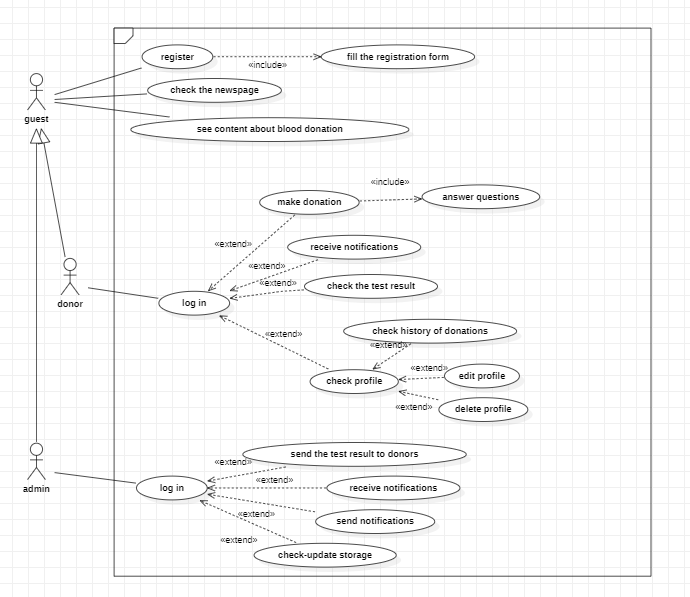
\includegraphics[width=1\textwidth]{images/use.png}
    \caption{Use Case Diagram}
    \label{fig:figure4}
\end{figure}



\section{Class Diagram}
\subsection{Definition}
A class diagram is a UML diagram used to model the structure of a system by showing the classes, attributes, methods, and relationships between them. It represents the static view of the system and provides a blueprint for the implementation of the system. Class diagrams are useful for visualizing and organizing complex systems in the design phase of software development.
\subsection{Class diagram of the application}

\begin{figure}[H]
    \centering
    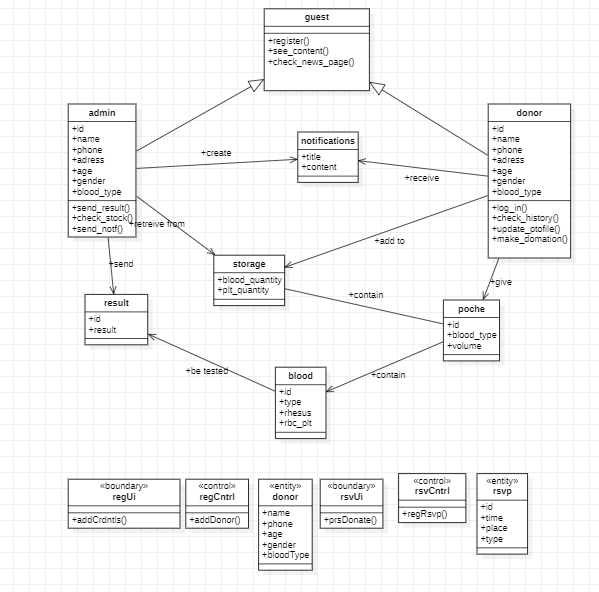
\includegraphics[width=1\textwidth]{images/niw.png}
    \caption{ Class Diagram}
    \label{fig:figure4}
\end{figure}

\section{Sequence Diagram}
\subsection{Definition}
A sequence diagram is a type of UML diagram used in software engineering to model the interactions between objects or components in a system. It represents a dynamic view of the system by showing the sequence of messages exchanged between objects and the order in which they occur. Sequence diagrams are useful for analyzing and designing systems that have complex interactions between different components or objects.
\subsection{Use Case Description}

\begin{figure}[H]
    \centering
    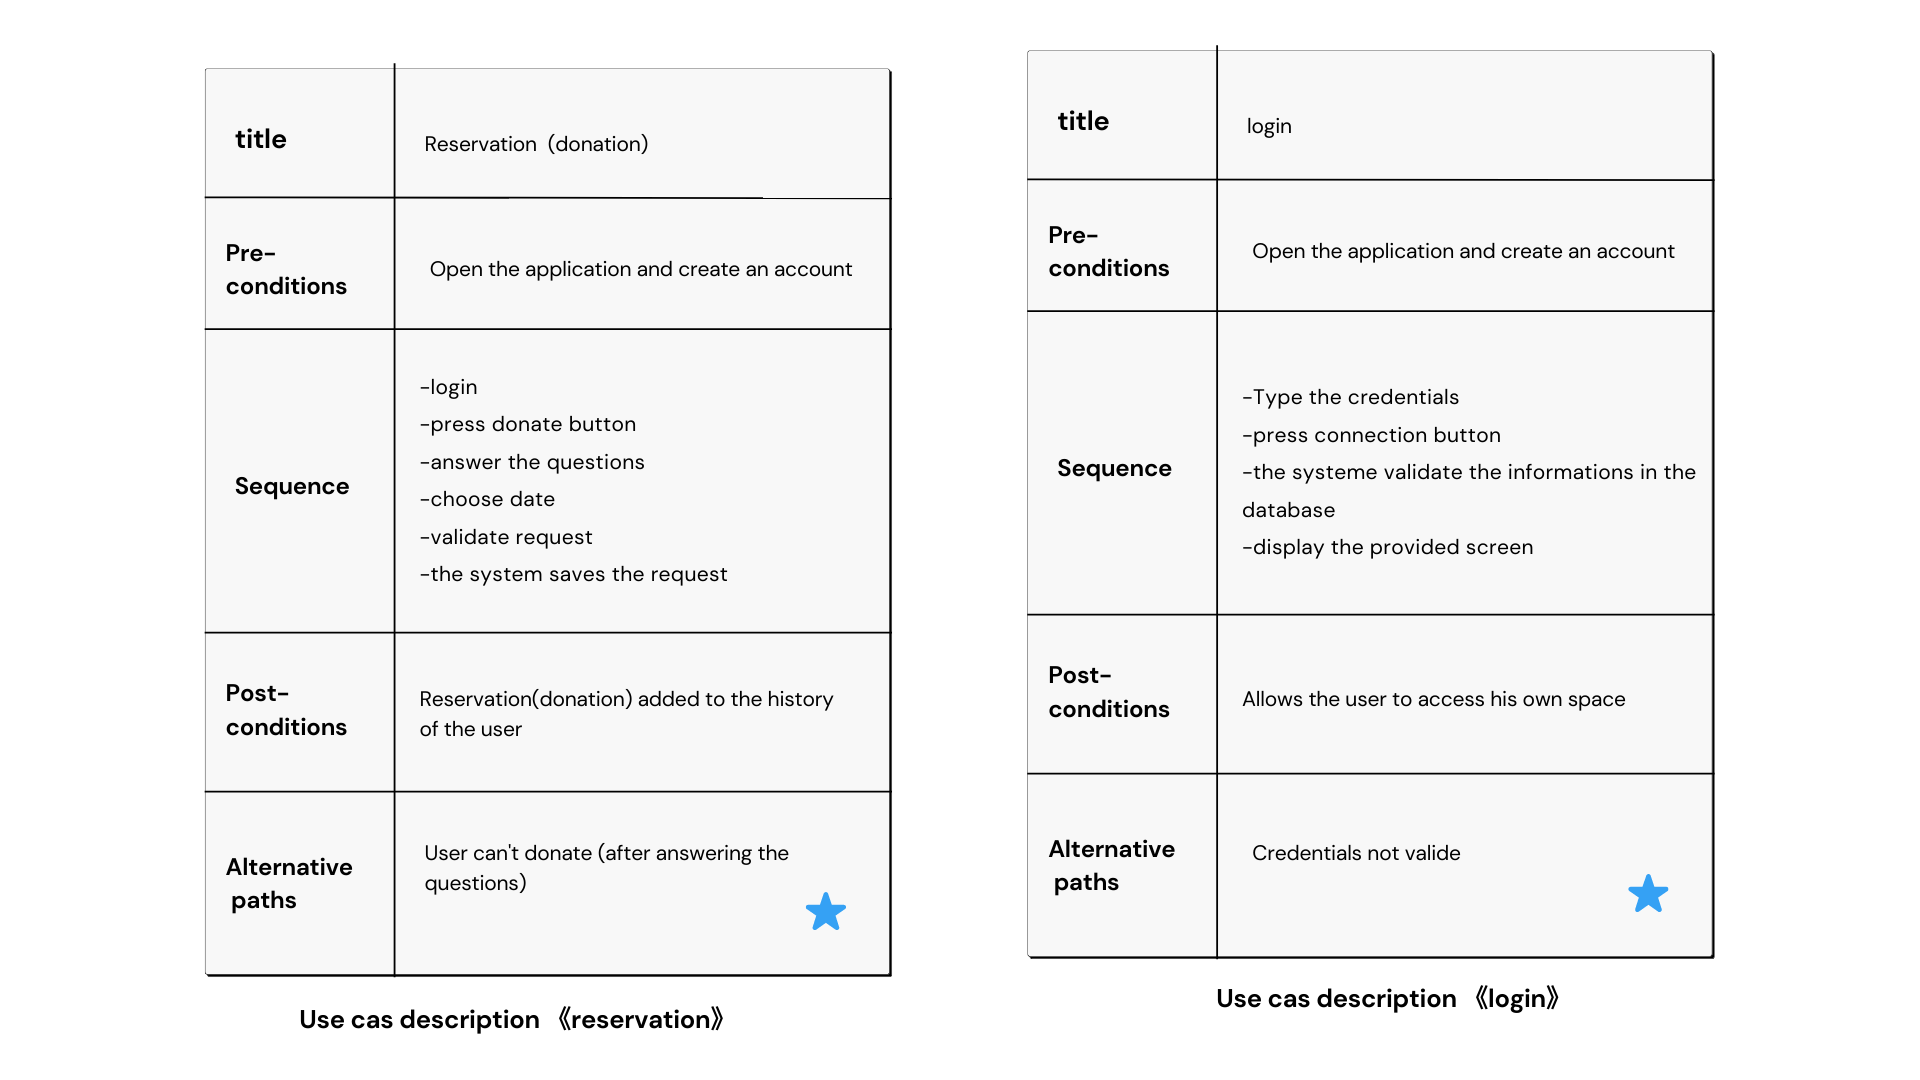
\includegraphics[width=1\textwidth]{images/Let's brainstorm for thoughts, ideas, and inspiration using an idea board..png}
    \caption{Use Case description}
    \label{fig:figure4}
\end{figure}
\subsection{Sequence Diagram of the Application}

\begin{figure}[H]
    \centering
    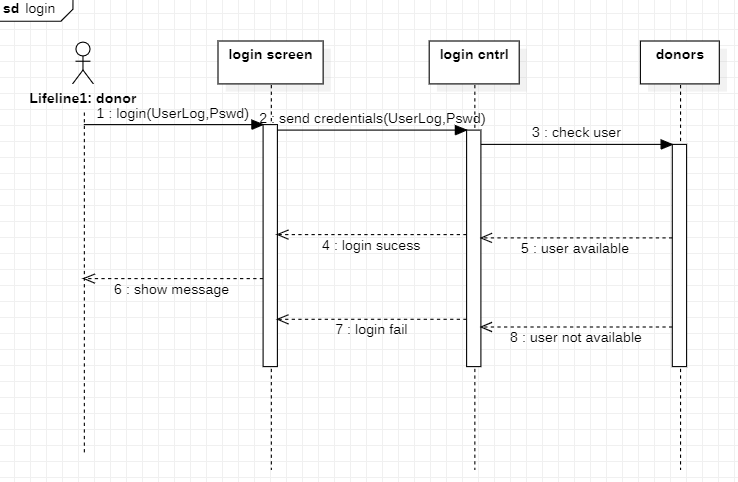
\includegraphics[width=1\textwidth]{images/login.png}
    \caption{ Login Sequence Diagram}
    \label{fig:figure4}
\end{figure}

\begin{figure}[H]
    \centering
    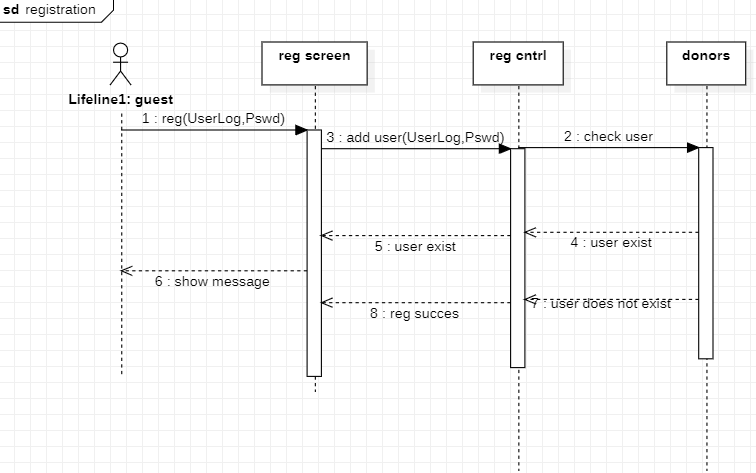
\includegraphics[width=1\textwidth]{images/regs.png}
    \caption{Registration Sequence Diagram}
    \label{fig:figure4}
\end{figure}

\begin{figure}[H]
    \centering
    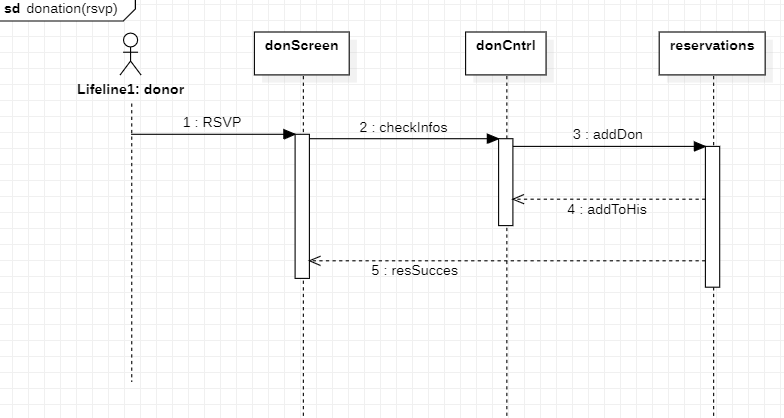
\includegraphics[width=1\textwidth]{images/don.png}
    \caption{Make Donation Sequence Diagram}
    \label{fig:figure4}
\end{figure}


%\section{Conclusion}

%that included various UML diagrams, including use case diagrams, %diagram classes, and sequence diagrams.

%The suggested conceptual solution will be presented in the following %chapter.




\chapter{Implementation}
\label{chp:paper02}
\section{Introduction}
After completing the design phase of the application, we will begin in this chapter the realization and implementation part by explaining the work environment and the selected development tools as well as the interfaces of our application.

At the end of this chapter, the objectives must have been achieved and the system must be ready to be exploited by end users.




\section{Development environment}

For the realization of our application, we used different tools and development software, tool for database management, modeling software, software for writing this report


\subsection{Adobe XD}
Adobe XD is a user experience design tool used to create wireframes, prototypes, and designs for digital products. It includes design and prototyping tools, collaboration features, and the ability to design for multiple devices and screen sizes. It's part of Adobe Creative Cloud, a subscription-based service for creative tools and services. \cite{adobe}
\begin{figure}[H]
    \centering
    
\includegraphics[width=0.3\textwidth]{images/Adobe_XD_CC_icon.svg.png}
    \caption{Adobe XD logo}
    \label{fig:figure4}
\end{figure}


\subsection{Visual Studio Code}
Visual Studio Code, also commonly referred to as VS Code, is a source-code editor made by Microsoft with the Electron Framework, for Windows, Linux and macOS.Features include support for debugging, syntax highlighting, intelligent code completion, snippets, code refactoring, and embedded Git. Users can change the theme, keyboard shortcuts, preferences, and install extensions that add functionality.

In the Stack Overflow 2022 Developer Survey, Visual Studio Code was ranked the most popular developer environment tool among 71,010 respondents, with 74.48 reporting that they use it.\cite{vscode}

\begin{figure}[H]
    \centering
    
\includegraphics[width=0.6\textwidth]{images/1_EOPCay4ML76rIUskd6ZwRg.png}
    \caption{visual studio code logo}
    \label{fig:figure4}
\end{figure}

\subsection{Flutter Framwork}
Flutter is an open-source mobile application development framework created by Google that allows developers to build native-looking, high-performance mobile applications for Android, iOS, and other platforms, using a single codebase. It's known for its ease of use, fast development times, and ability to create beautiful and responsive UI designs. \cite{flutter}
\begin{figure}[H]
    \centering
    
\includegraphics[width=0.5\textwidth]{images/c823e53b3a1a7b0d36a9.png}
    \caption{flutter logo}
    \label{fig:figure4}
\end{figure}

\subsection{Dart Language}
Dart is a general-purpose, object-oriented programming language created by Google that's designed to be fast, efficient, and easy to learn. It's used for a wide range of applications, from web and mobile development to server-side programming, and is the primary language used to develop applications with Google's Flutter framework.\cite{dart}
\begin{figure}[H]
    \centering
    
\includegraphics[width=0.5\textwidth]{images/Dart_programming_language_logo.svg.png}
    \caption{dart language logo}
    \label{fig:figure4}
\end{figure}

\subsection{Firebase}
Firebase is a cloud-based mobile and web application development platform developed by Google that provides a comprehensive set of services and tools to help developers build high-quality, scalable applications quickly and easily. It includes a real-time database, authentication, hosting, cloud functions, and more, and enables developers to store and manage data in real-time, run server-side code in response to events, and deploy web applications to the cloud with ease.\cite{firebase}
\begin{figure}[H]
    \centering
    
\includegraphics[width=0.5\textwidth]{images/512px-Firebase_Logo.svg.png}
    \caption{firebase logo}
    \label{fig:figure4}
\end{figure}

\subsection{BlueStacks}
BlueStacks is a popular Android emulator software that allows users to run Android applications on their desktop or laptop computers. It creates a virtual Android device on the user's computer, enabling them to interact with Android apps using their mouse, keyboard, and other peripherals. BlueStacks supports a wide range of Android apps and provides a seamless and immersive Android experience on desktop and laptop computers.\cite{bluestacks}
\begin{figure}[h]
    \centering
    
\includegraphics[width=0.5\textwidth]{images/e634679eb4e06627c42ca5667d83e88e.png}
    \caption{BlueStacks logo}
    \label{fig:figure4}
\end{figure}

\subsection{StarUML}
StarUML is a popular open-source UML modeling tool that helps developers create high-quality software designs using a variety of UML diagrams. It provides advanced features such as model validation, code generation, and round-trip engineering, and is widely used in software development projects for its flexibility, extensibility, and ease-of-use. StarUML is available for Windows, Mac, and Linux platforms and helps developers create high-quality software designs efficiently and effectively.
\begin{figure}[h]
    \centering
    
\includegraphics[width=0.5\textwidth]{images/Ey8OGaPWUAAfrVX.jpg}
    \caption{StarUML logo}
    \label{fig:figure4}
\end{figure}


\subsection{Latex }
The report was written using LaTeX, which is both a language and a document composition system. It allows for automatic document layout adhering to typographical norms, and is known for its mathematical mode which allows for complex formulas to be easily composed. LaTeX is popular in technical and scientific fields, and is often used for medium or large-sized documents such as articles, theses, and books.
\begin{figure}[H]
    \centering
    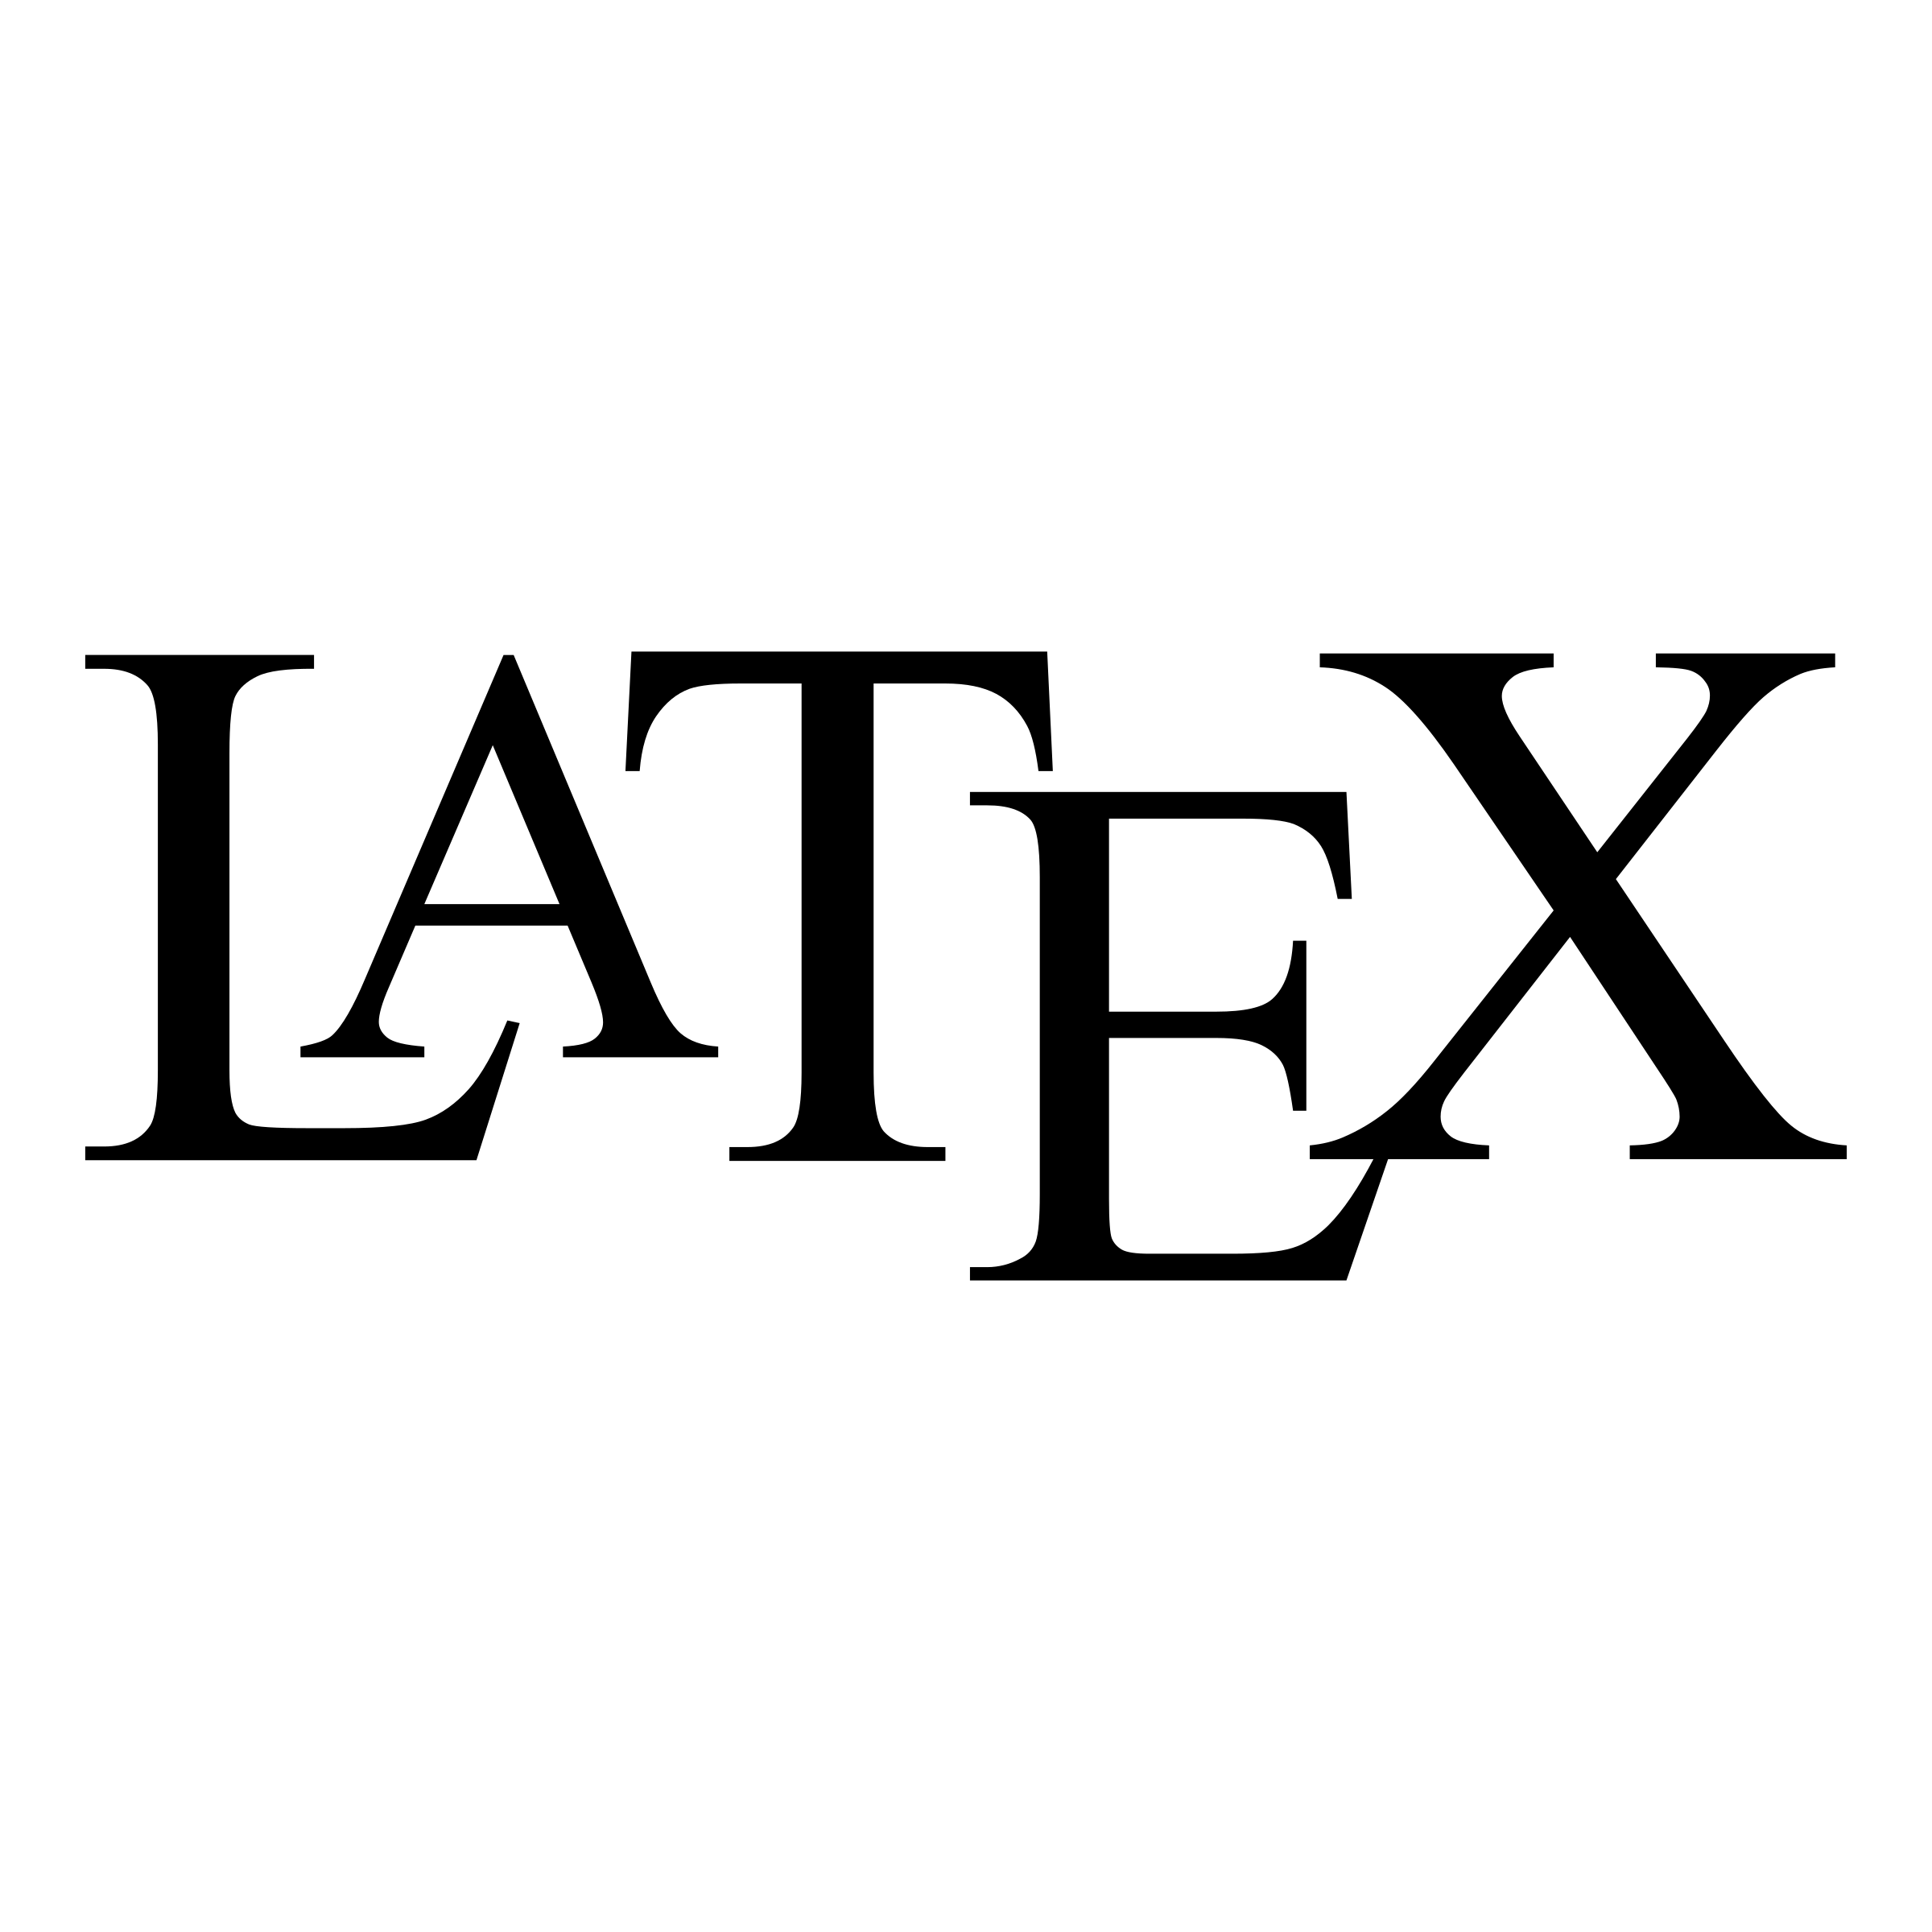
\includegraphics[width=0.5\textwidth]{images/latex-logo-png-transparent.png}
    \caption{Latex logo}
    \label{fig:figure4}
\end{figure}

\subsection{Overleaf }

Overleaf is a web-based platform for writing and collaborating on LaTeX documents. It offers a variety of features including real-time collaboration, automatic document backups, and a wide range of templates and examples. Overleaf simplifies the process of writing LaTeX documents by providing an intuitive user interface and a variety of helpful tools and resources. In our case, we used Overleaf to write and collaborate on this report, taking advantage of its features and functionality to streamline the writing and editing document and save it PDF.\cite{overleaf}
\begin{figure}[H]
    \centering
    
\includegraphics[width=0.5\textwidth]{images/overleaf_wide_colour_light_bg.png}
    \caption{Latex logo}
    \label{fig:figure4}
\end{figure}



\section{Graphic Charter}
The graphic chart and design of an app play a crucial role in creating a strong visual identity and enhancing user experience,conveying the app's message, and enhancing usability for donors and users,in this part we will see what we used in our application "drop angel" .
    \begin{figure}[H]
    \centering
    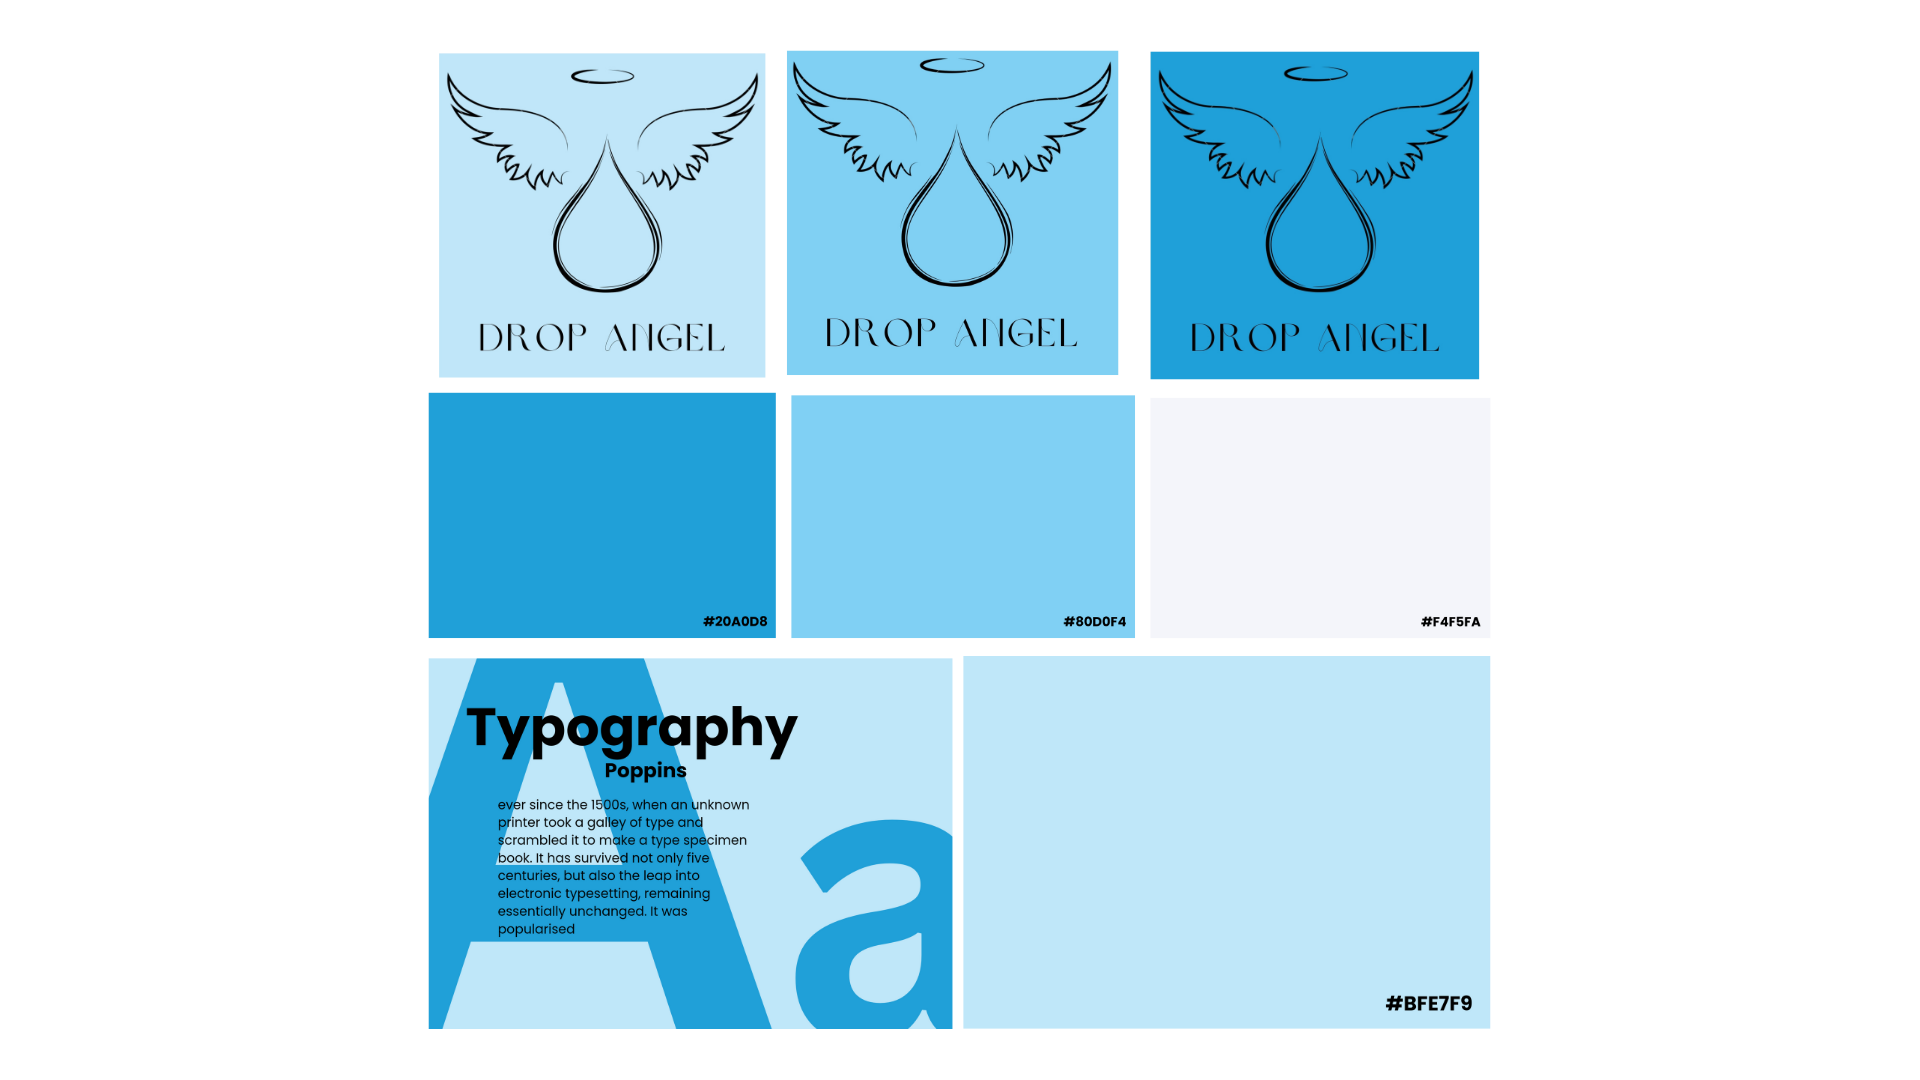
\includegraphics[width=1.15\textwidth]{images/Let's brainstorm for thoughts, ideas, and inspiration using an idea board. (3).png}
    \caption{graphic charter}
    \label{fig:figure4}
\end{figure}


\subsection{Colors }
Choosing a specific color scheme for an application can have a significant impact on user engagement and overall brand identity. In the case of a blood donation app, the color blue can be a compelling choice. Blue is often associated with trust, reliability, and professionalism, making it an ideal color for a healthcare-related application. Additionally, blue is known to have a calming effect on the mind and body, which can be beneficial for users who may be anxious or hesitant about donating blood. Overall, the choice of blue as the primary color for a blood donation app can help to establish a sense of trust, professionalism, and calmness, while also conveying the seriousness and importance of the cause.


\begin{figure}[H]
\begin{subfigure}{.5\textwidth}
  \centering
  % include first image
  
\includegraphics[width=.9\linewidth]{images/color1.png}  
  \caption{Main color 1}
  \label{fig:sub-first}
\end{subfigure}
\begin{subfigure}{.5\textwidth}
  \centering
  % include second image
  
\includegraphics[width=.9\linewidth]{images/4.png}  
  \caption{Main color 2}
  \label{fig:sub-second}
\end{subfigure}
%\newline %\newline
\begin{subfigure}{.5\textwidth}
  \centering
  % include third image
  
\includegraphics[width=.9\linewidth]{images/3.png} 
  \caption{Main color 3}
  \label{fig:sub-third}
\end{subfigure}
\begin{subfigure}{.5\textwidth}
  \centering
  % include fourth image
  
\includegraphics[width=.9\linewidth]{images/5.png} 
  \caption{Main color 4}
  \label{fig:sub-fourth}
\end{subfigure}
\caption{Main Colors}
\label{fig:fig}
\end{figure}


\subsection{Logo }

\begin{figure}[H]
    \centering
    
\includegraphics[width=0.6\textwidth]{images/logo.png}
    \caption{Drop Angel logo}
    \label{fig:figure4}
\end{figure}
A logo can play a crucial role in creating a strong visual identity and communicating the app's message to its users that why we decided to create a logo for our application "Drop Angel" that features a drop of blood with angel wings,We chose this design because it is a powerful symbol of hope, compassion, and urgency. The combination of the angel wings and the drop of blood can create an emotional connection with users, making them more likely to engage with the app and support its mission. We believe that the logo will effectively convey the message that blood donation can save lives and encourage potential donors to take action.


\subsection{Typography}

\begin{figure}[H]
    \centering
    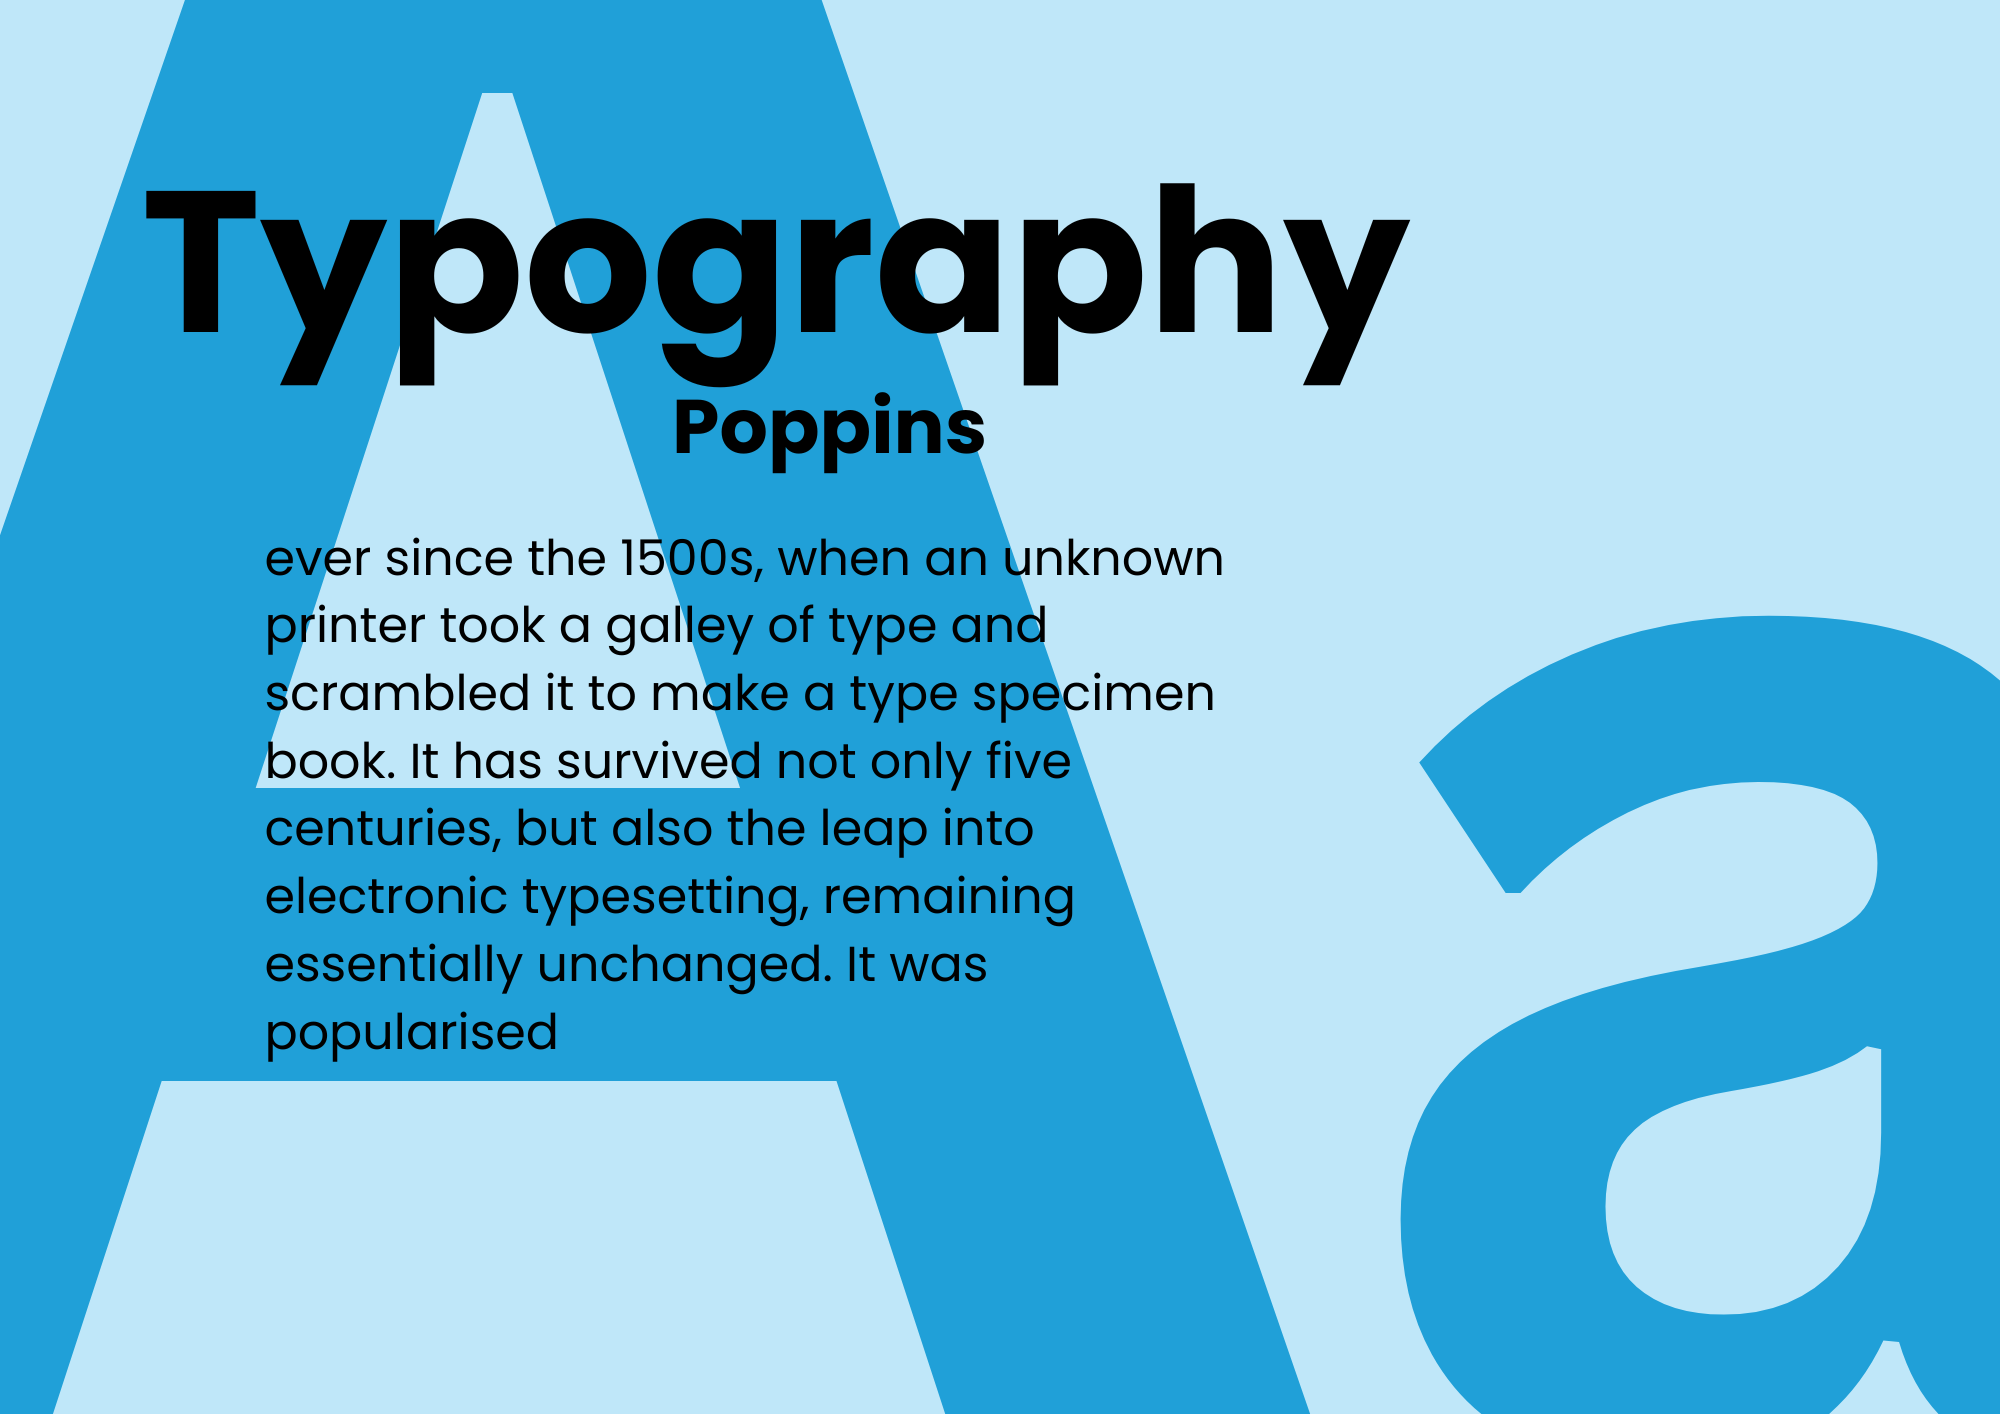
\includegraphics[width=0.7\textwidth]{images/1.png}
    \caption{Typography (Poppins)}
    \label{fig:figure4}
\end{figure}






\section{ Application Interfaces}







\begin{figure}[H]
	\hspace{1cm}
	\begin {minipage}[t]{4cm}
	\centering
	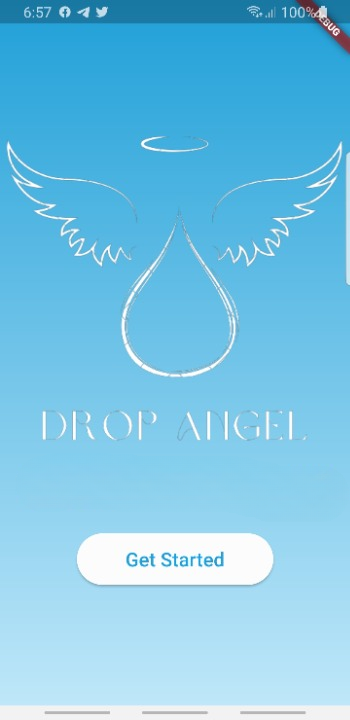
\includegraphics [ width =6 cm ]{images1/welcom_cleanup.jpg}
	\end {minipage}
	\hspace{2.5cm}
	\begin {minipage}[t]{4cm}
	\raggedright
	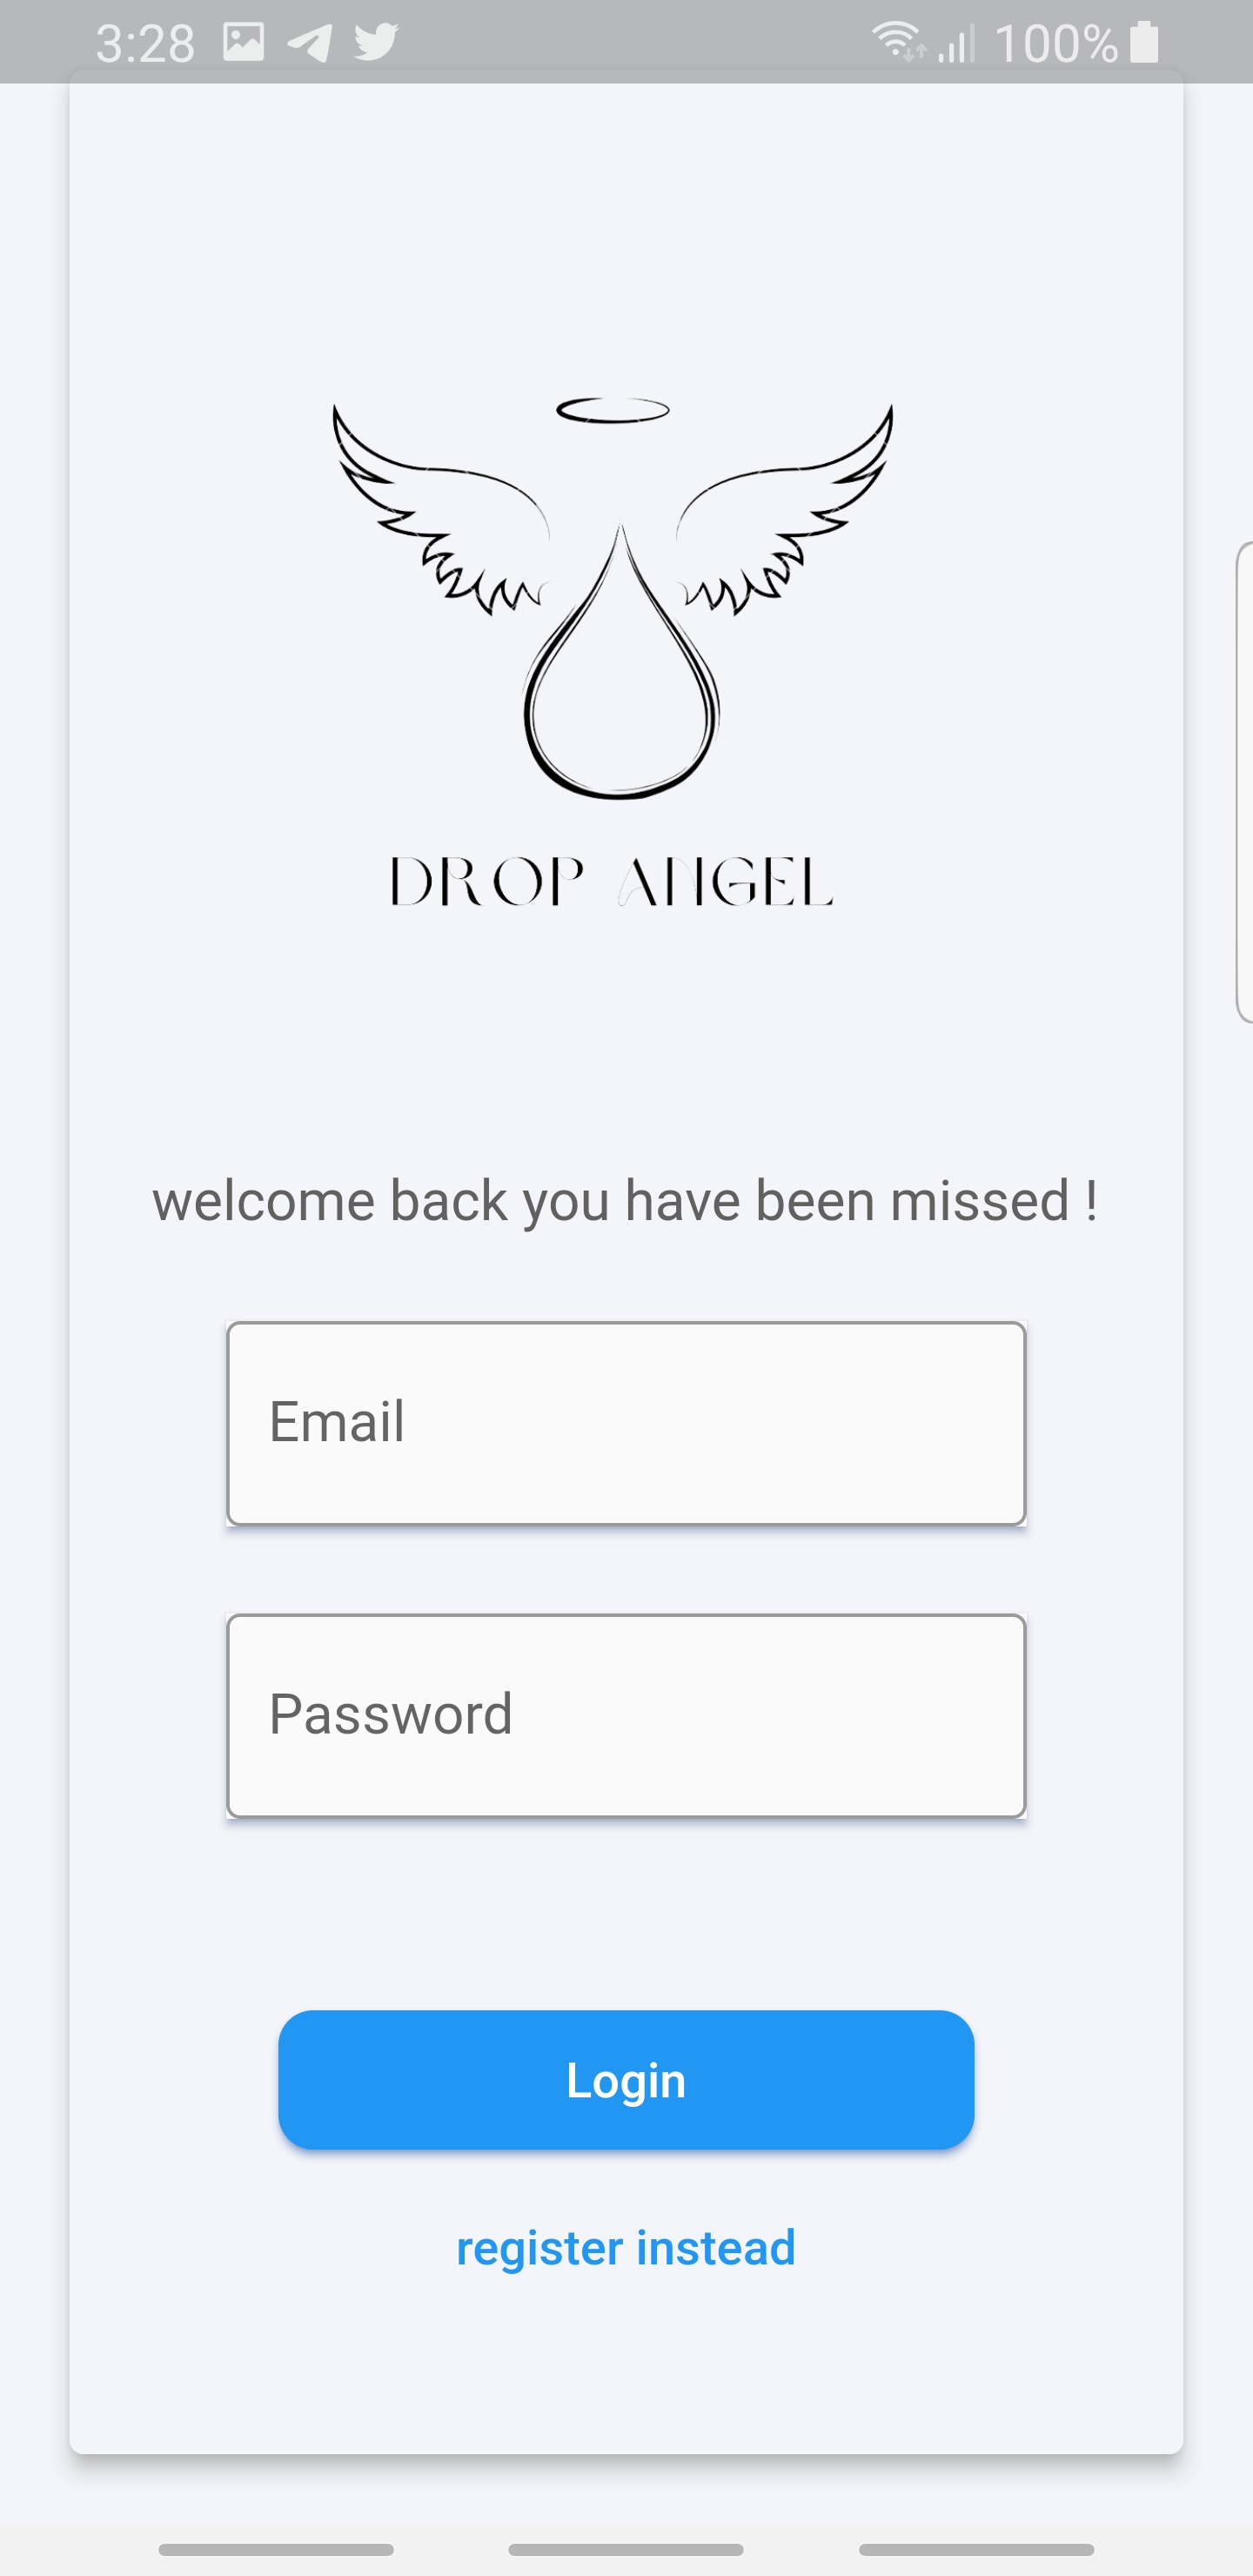
\includegraphics [ width =6 cm ]{images1/login.jpg}
	\end {minipage}
	\caption{Start pages}
\end{figure}




\begin{figure}[H]
	\hspace{1cm}
	\begin {minipage}[t]{4cm}
	\centering
	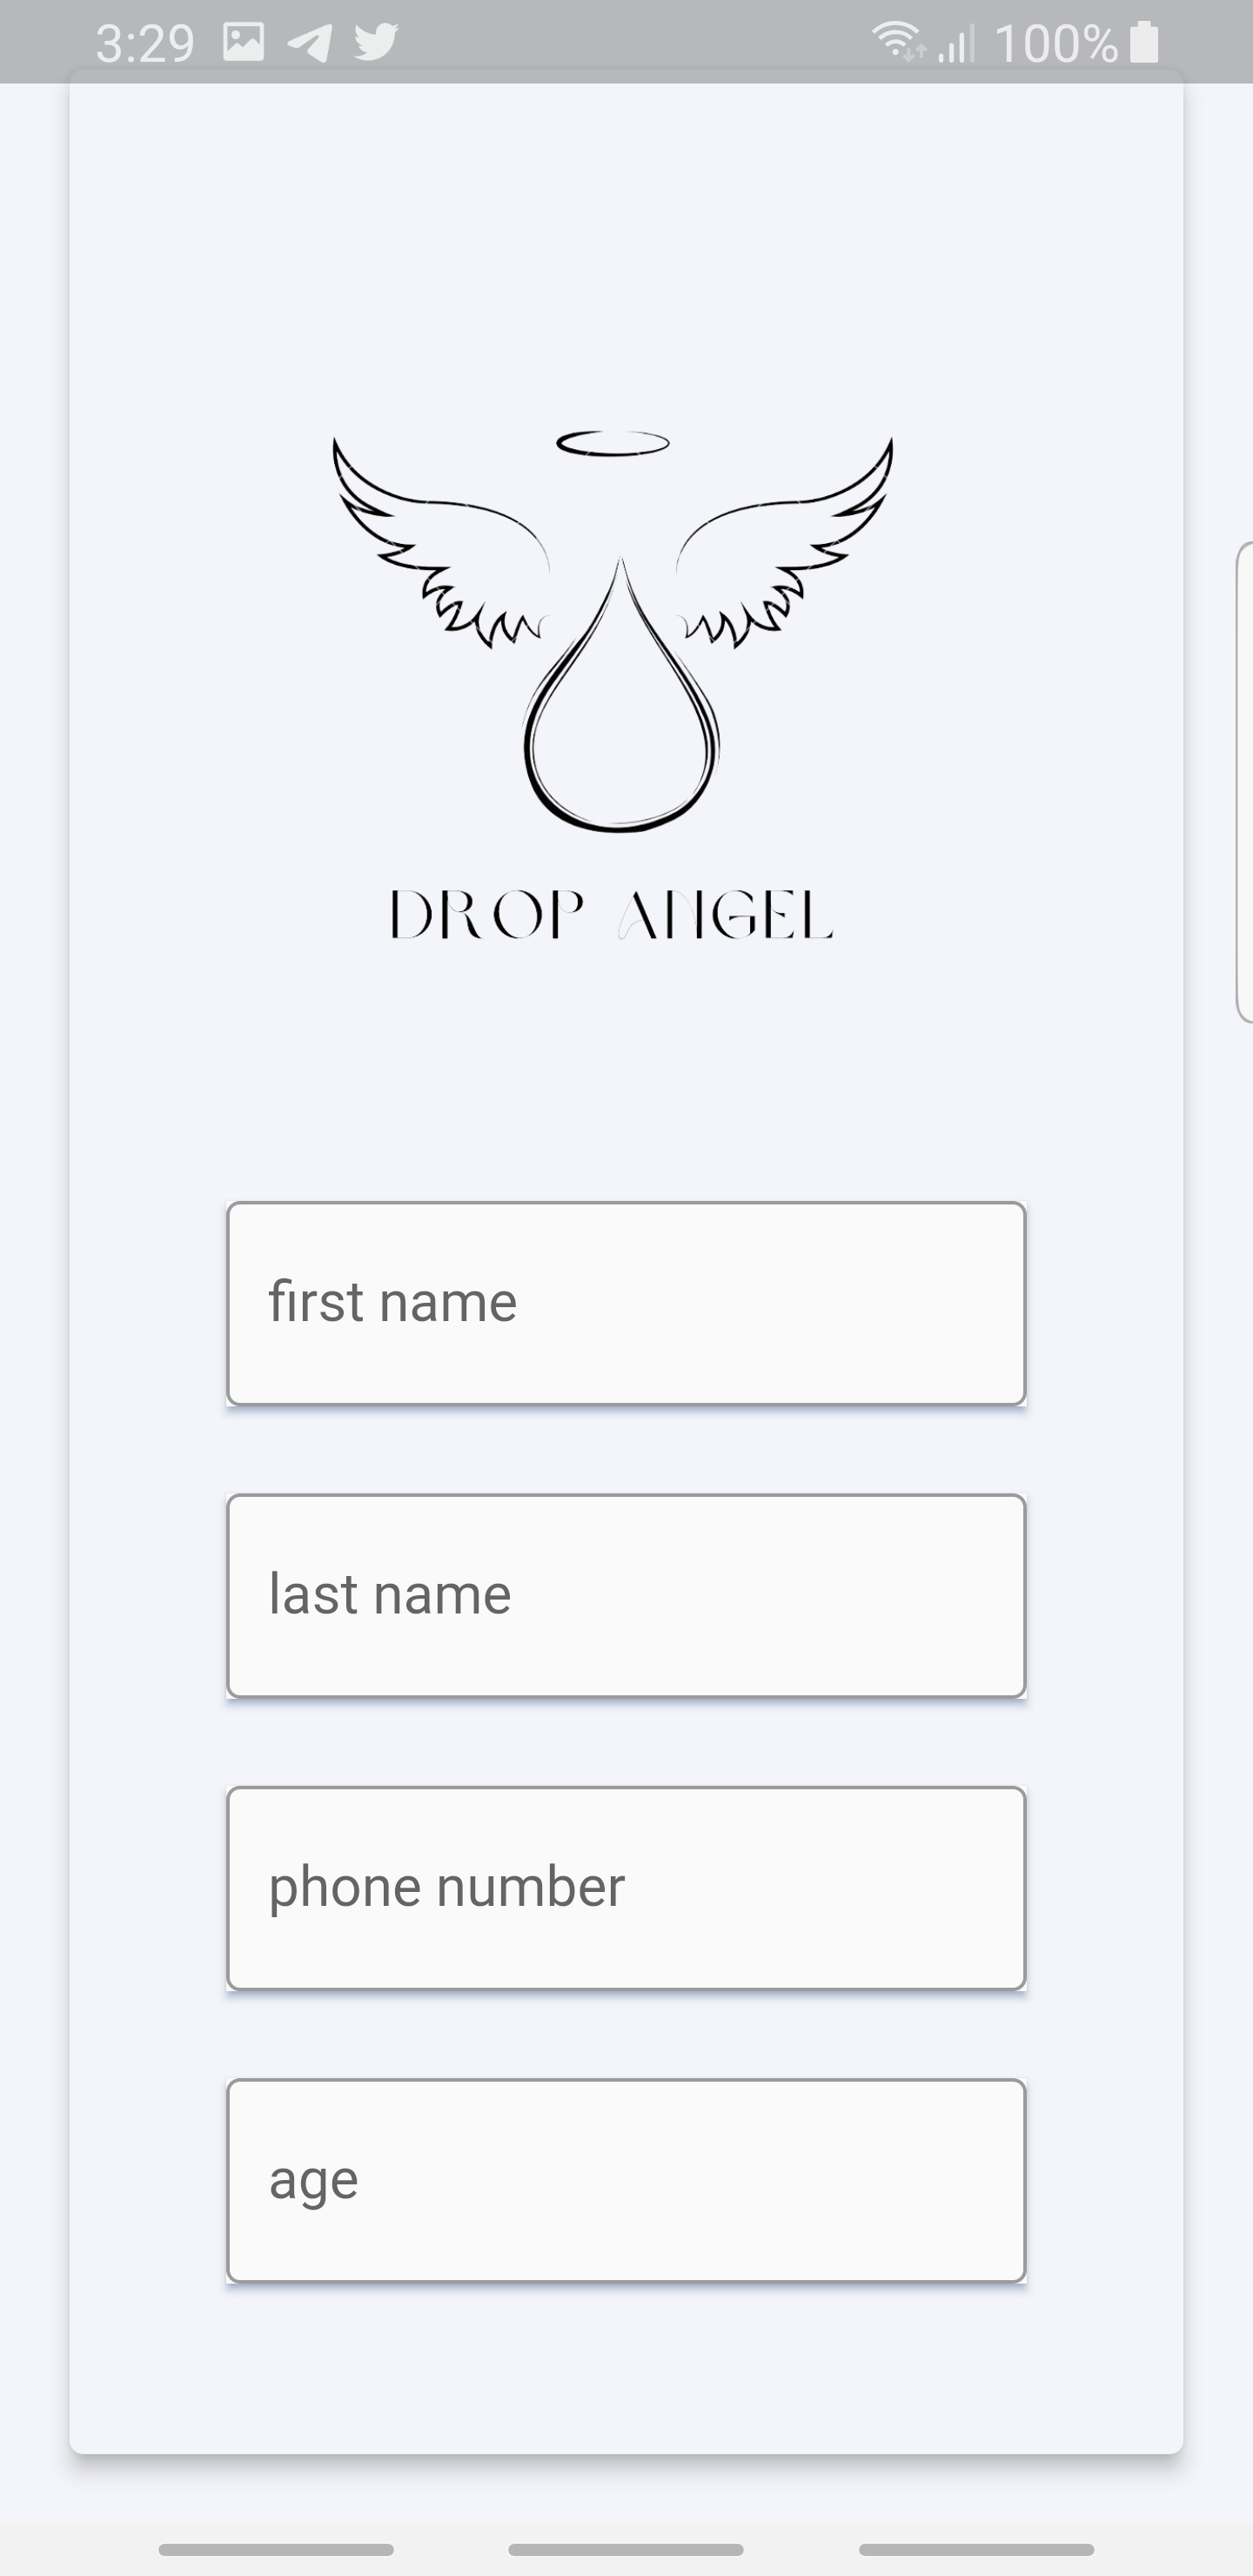
\includegraphics [ width =6 cm ]{images1/register1.jpg}
	\end {minipage}
	\hspace{2.5cm}
	\begin {minipage}[t]{4cm}
	\raggedright
	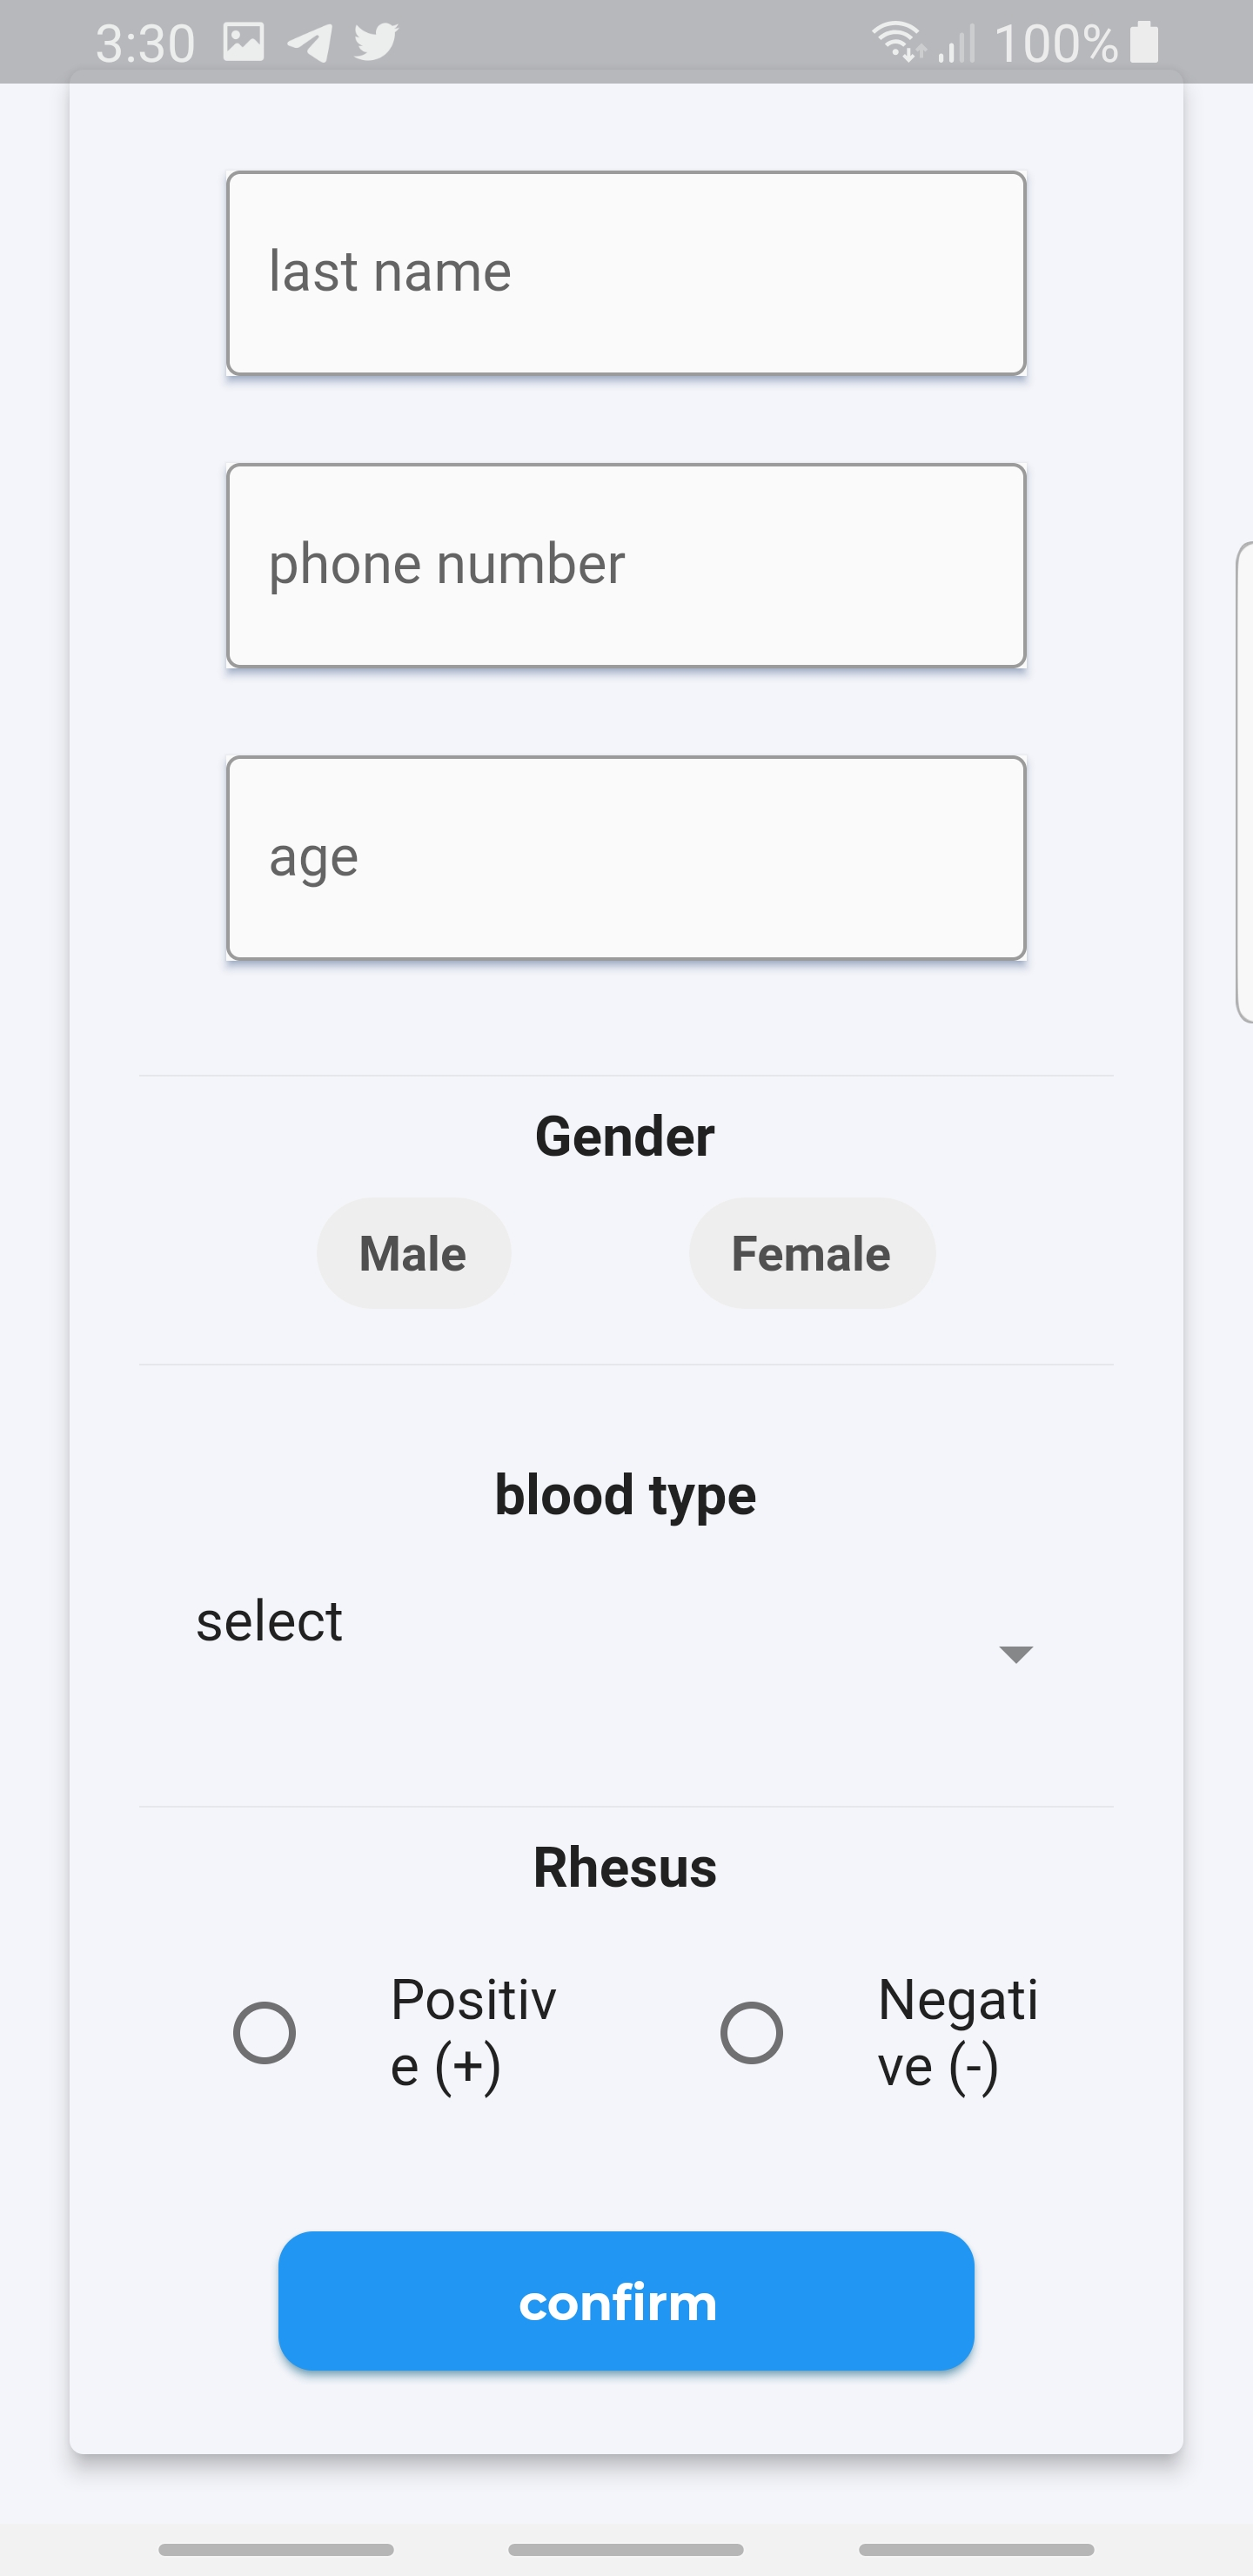
\includegraphics [ width =6 cm ]{images1/register2.jpg}
	\end {minipage}
	\caption{Registration }
\end{figure}


\begin{figure}
\begin{subfigure}{.31\textwidth}
  \centering
  % include first image
  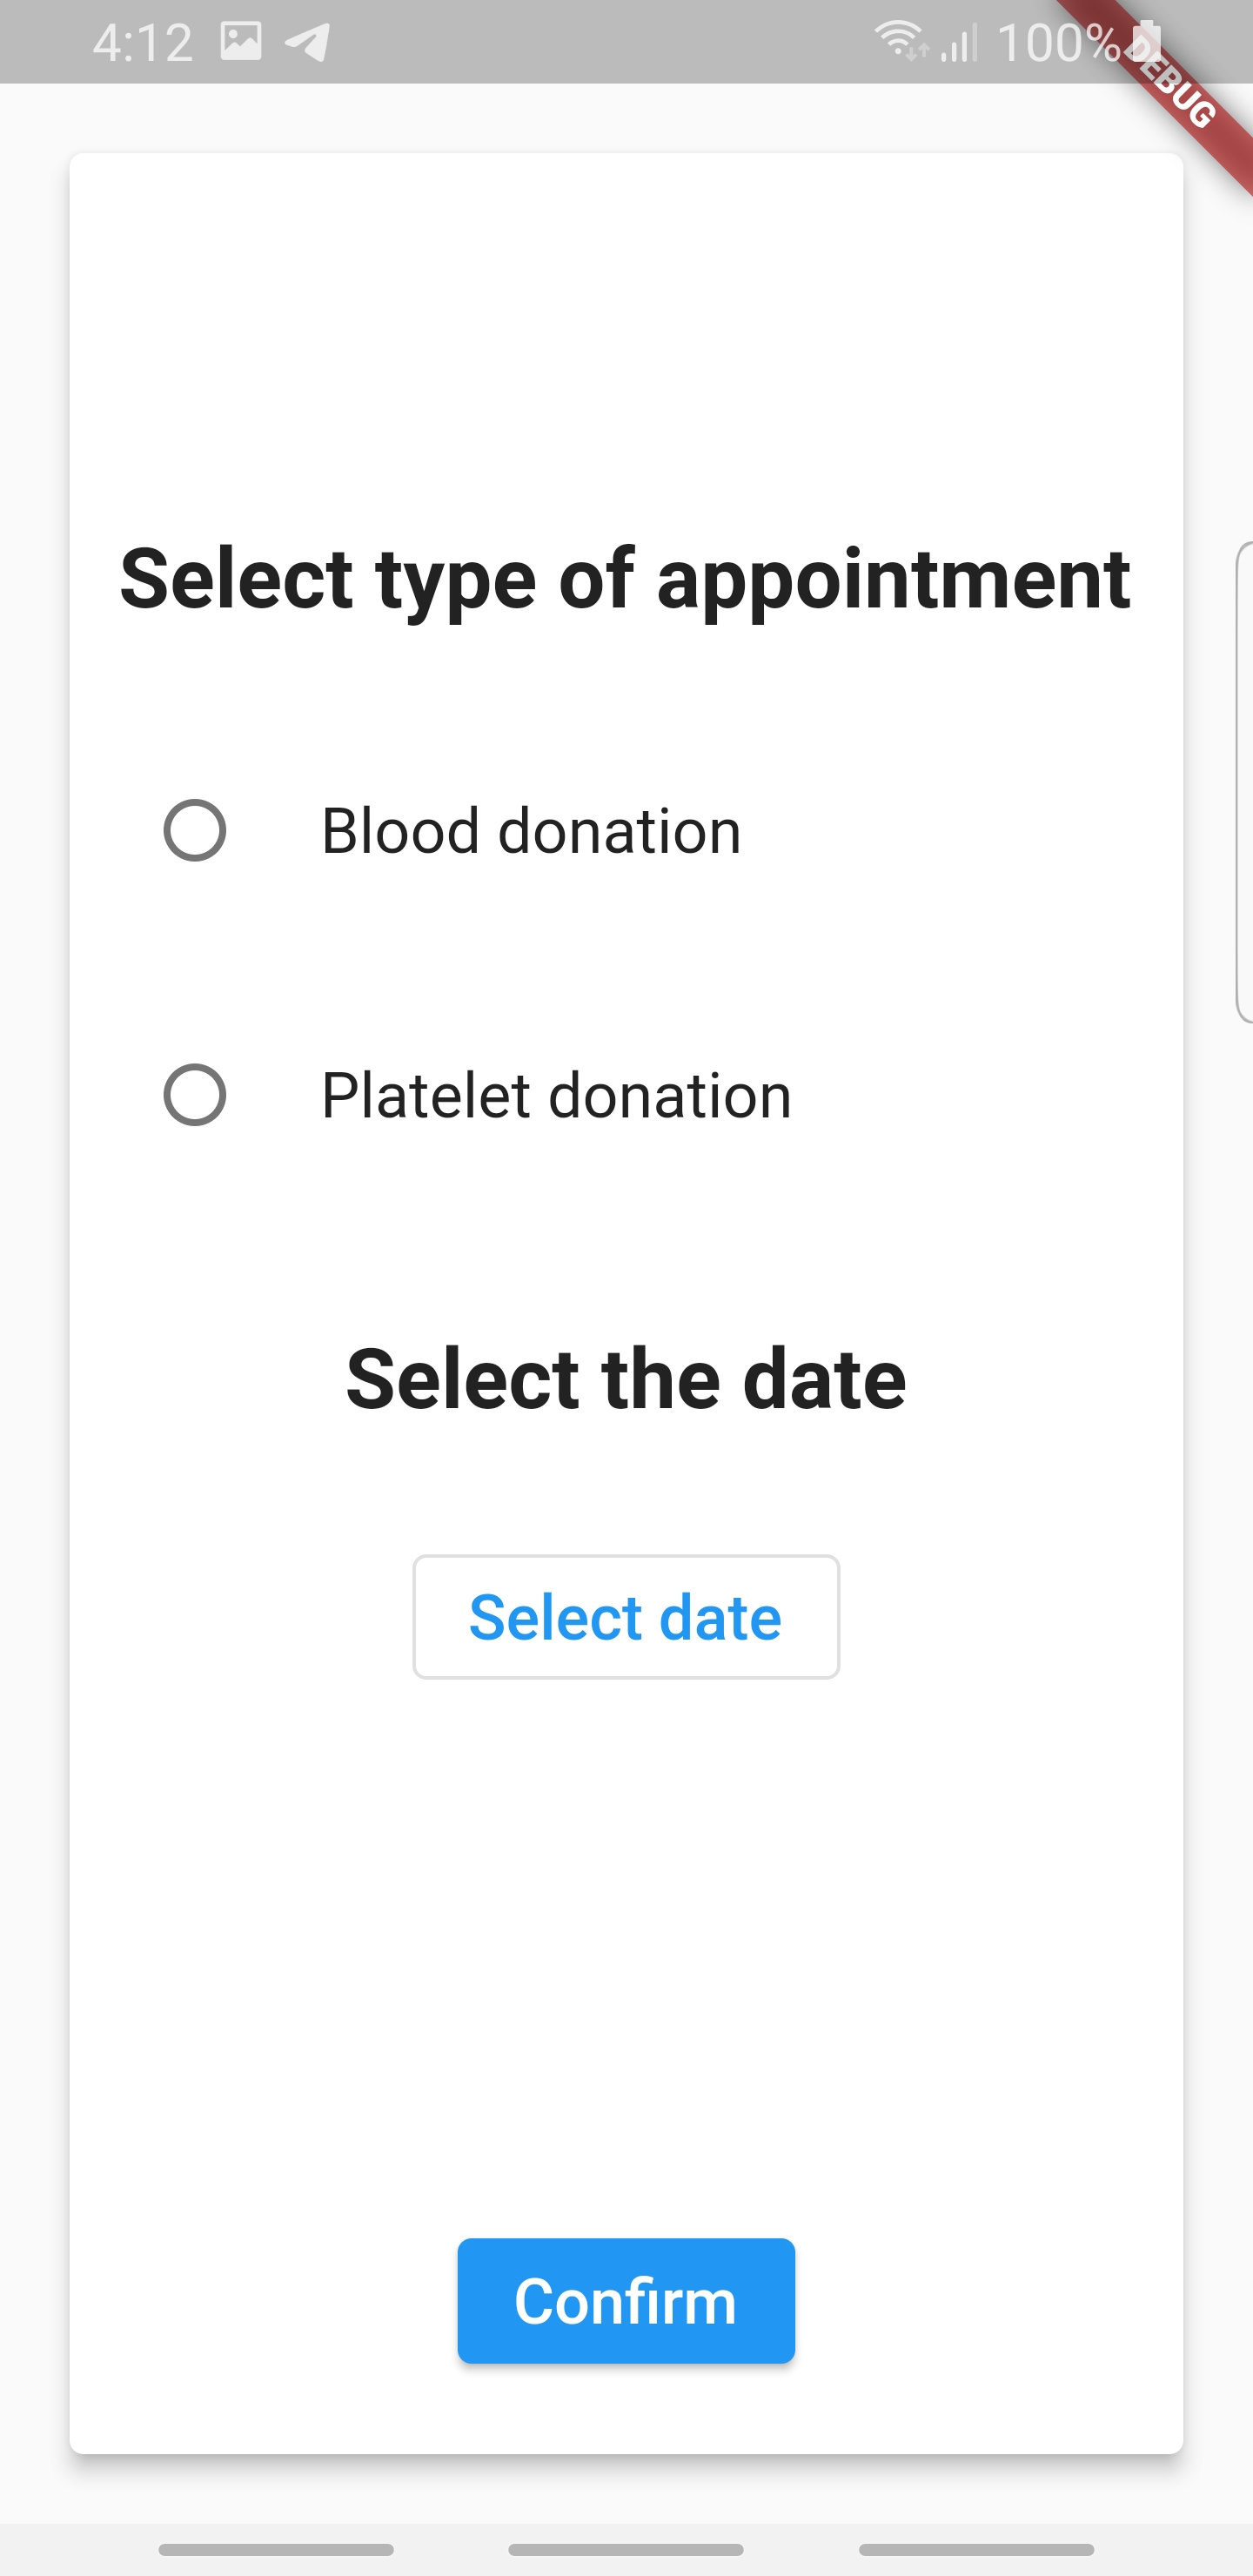
\includegraphics[width=1\linewidth]{images1/quess5.jpg}  
  %\caption{Put your sub-caption here}
  \label{fig:sub-first}
\end{subfigure}
\begin{subfigure}{.31\textwidth}
  \centering
  % include second image
  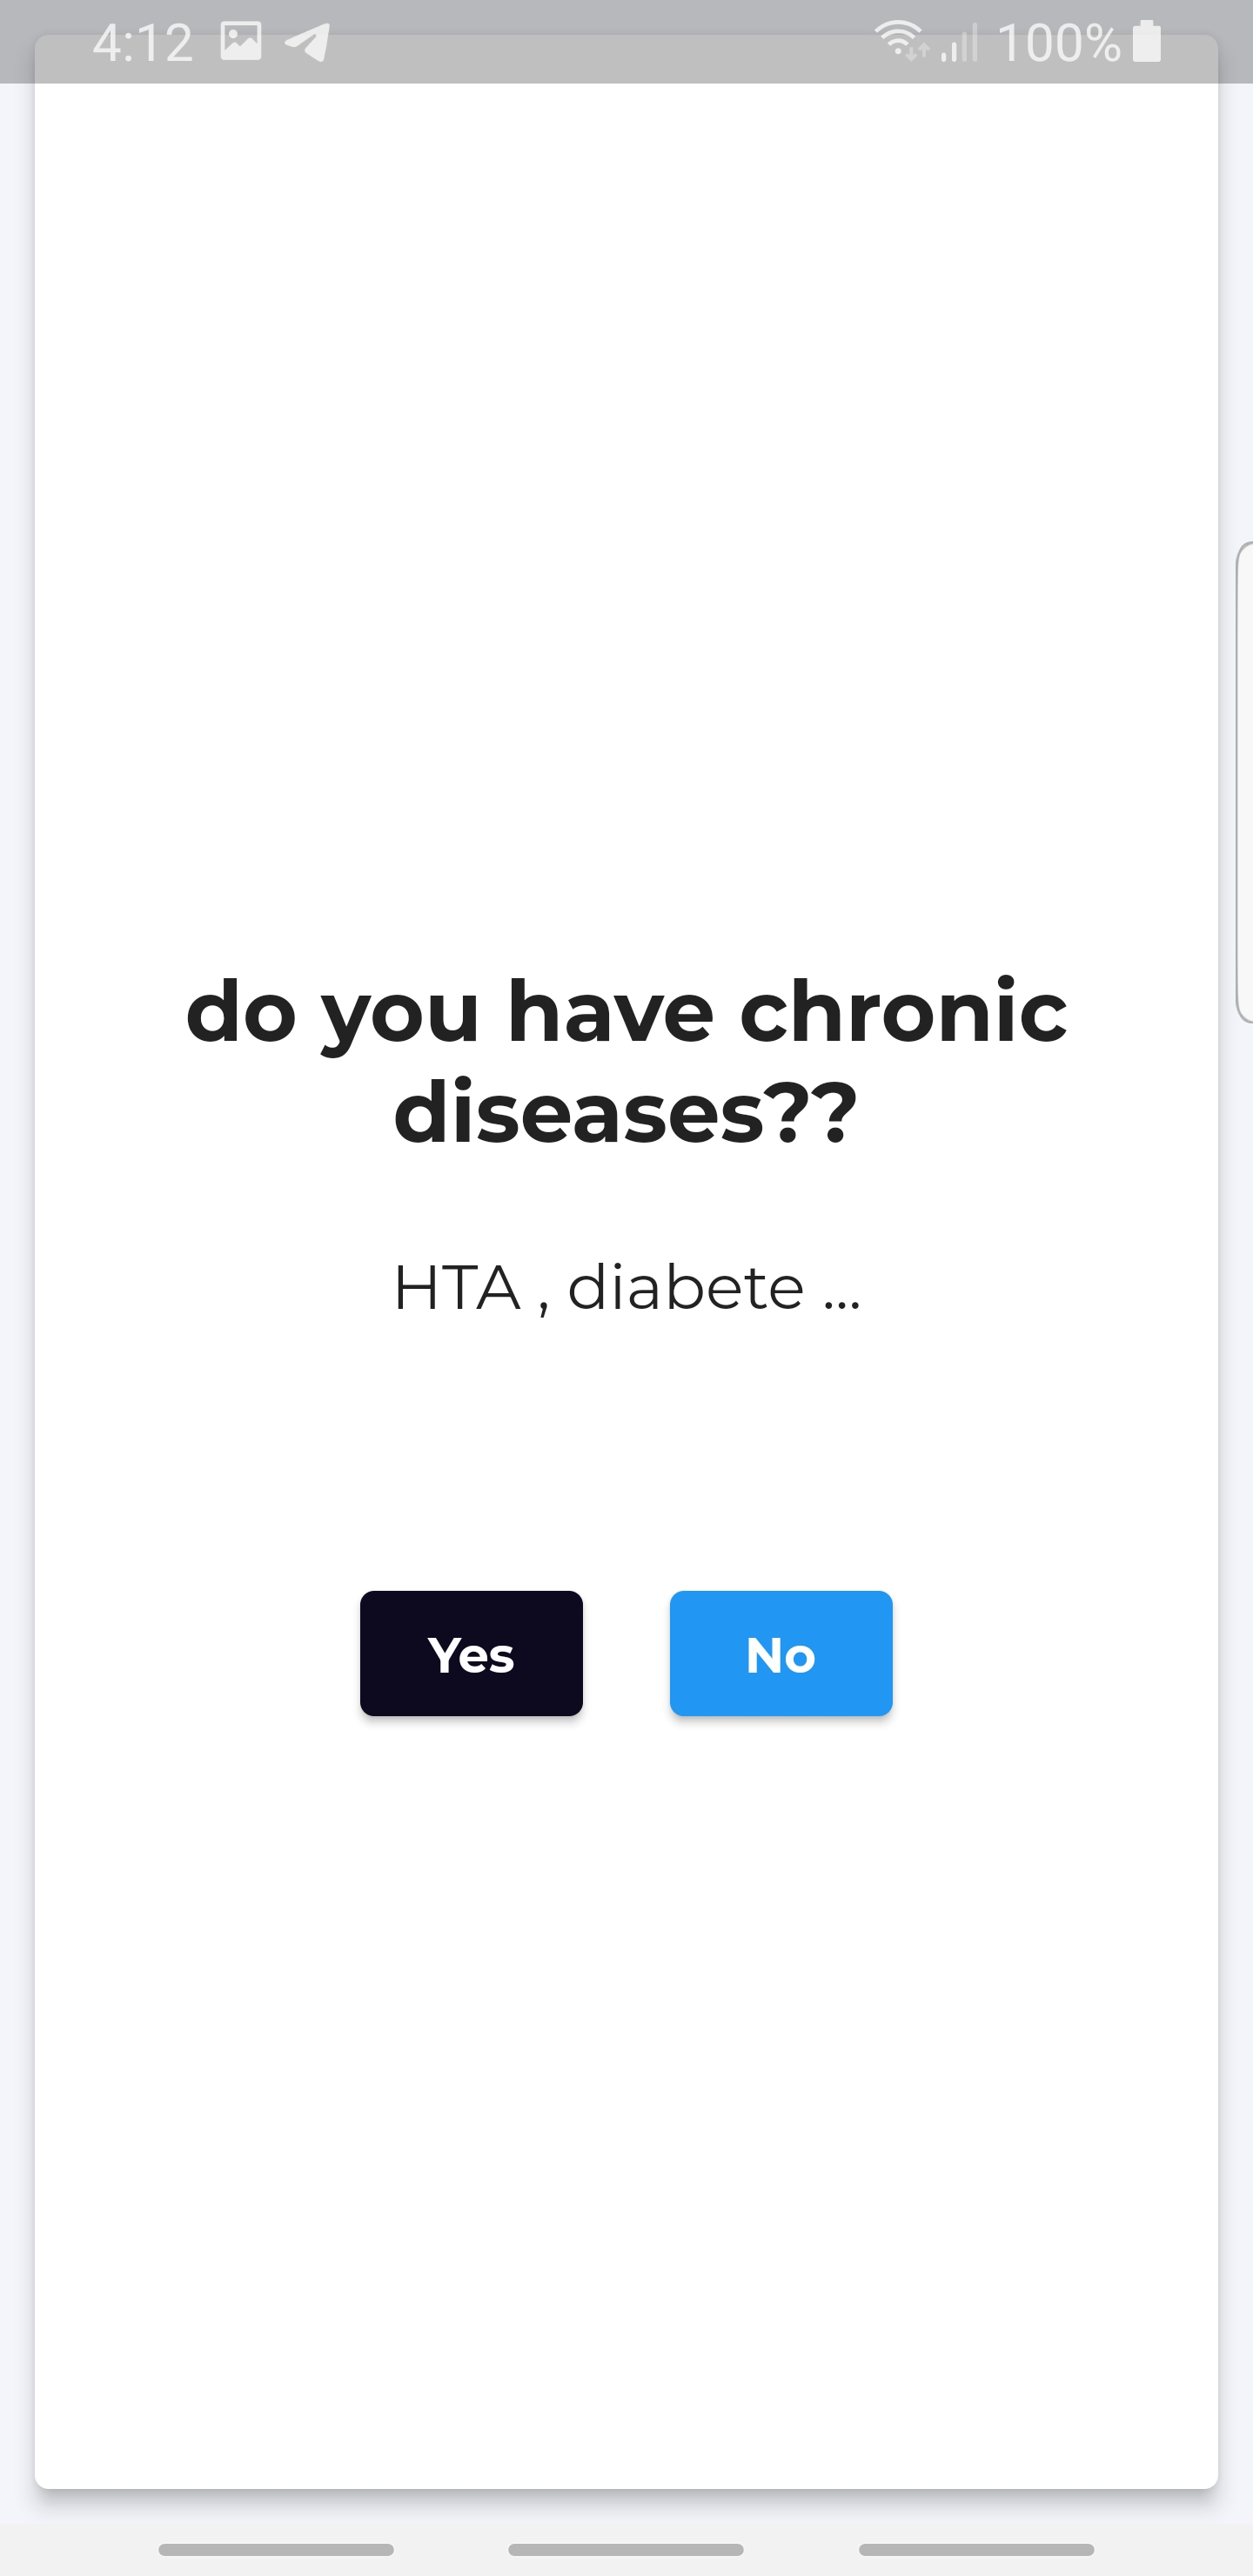
\includegraphics[width=1\linewidth]{images1/quess2.jpg}  
  %\caption{Put your sub-caption here}
  \label{fig:sub-second}
\end{subfigure}
\begin{subfigure}{.31\textwidth}
  \centering
  % include third image
  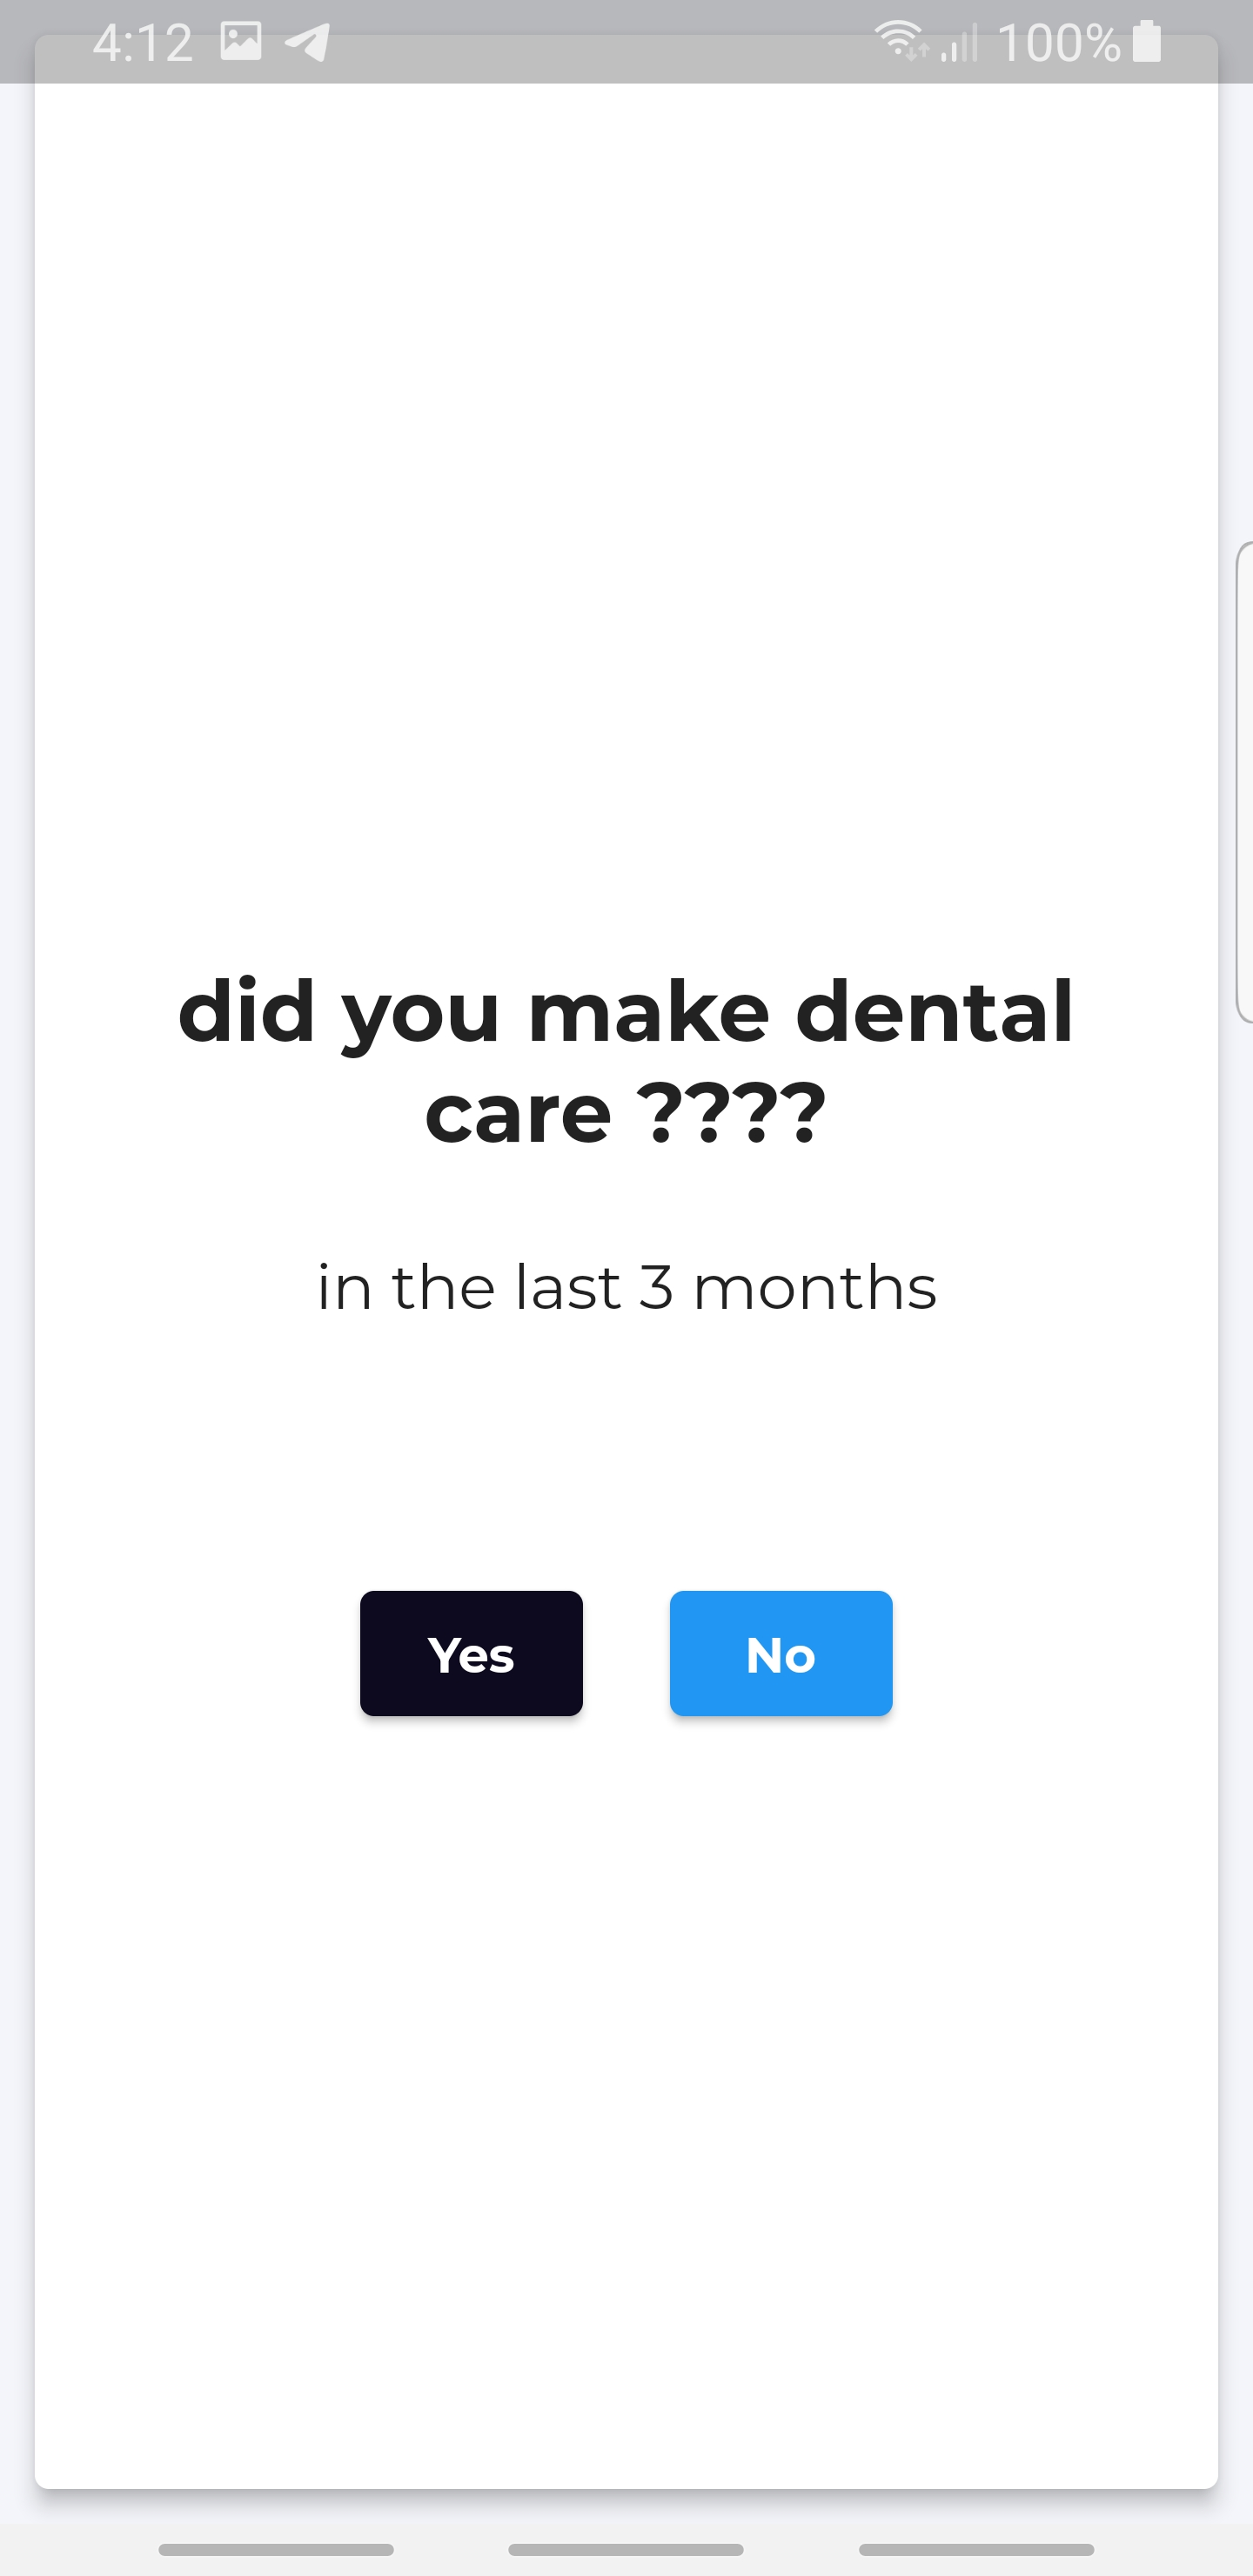
\includegraphics[width=1\linewidth]{images1/quess3.jpg}  
  %\caption{Put your sub-caption here}
  \label{fig:sub-third}
\end{subfigure}
\newline
\begin{subfigure}{.31\textwidth}
  \centering
  % include fourth image
  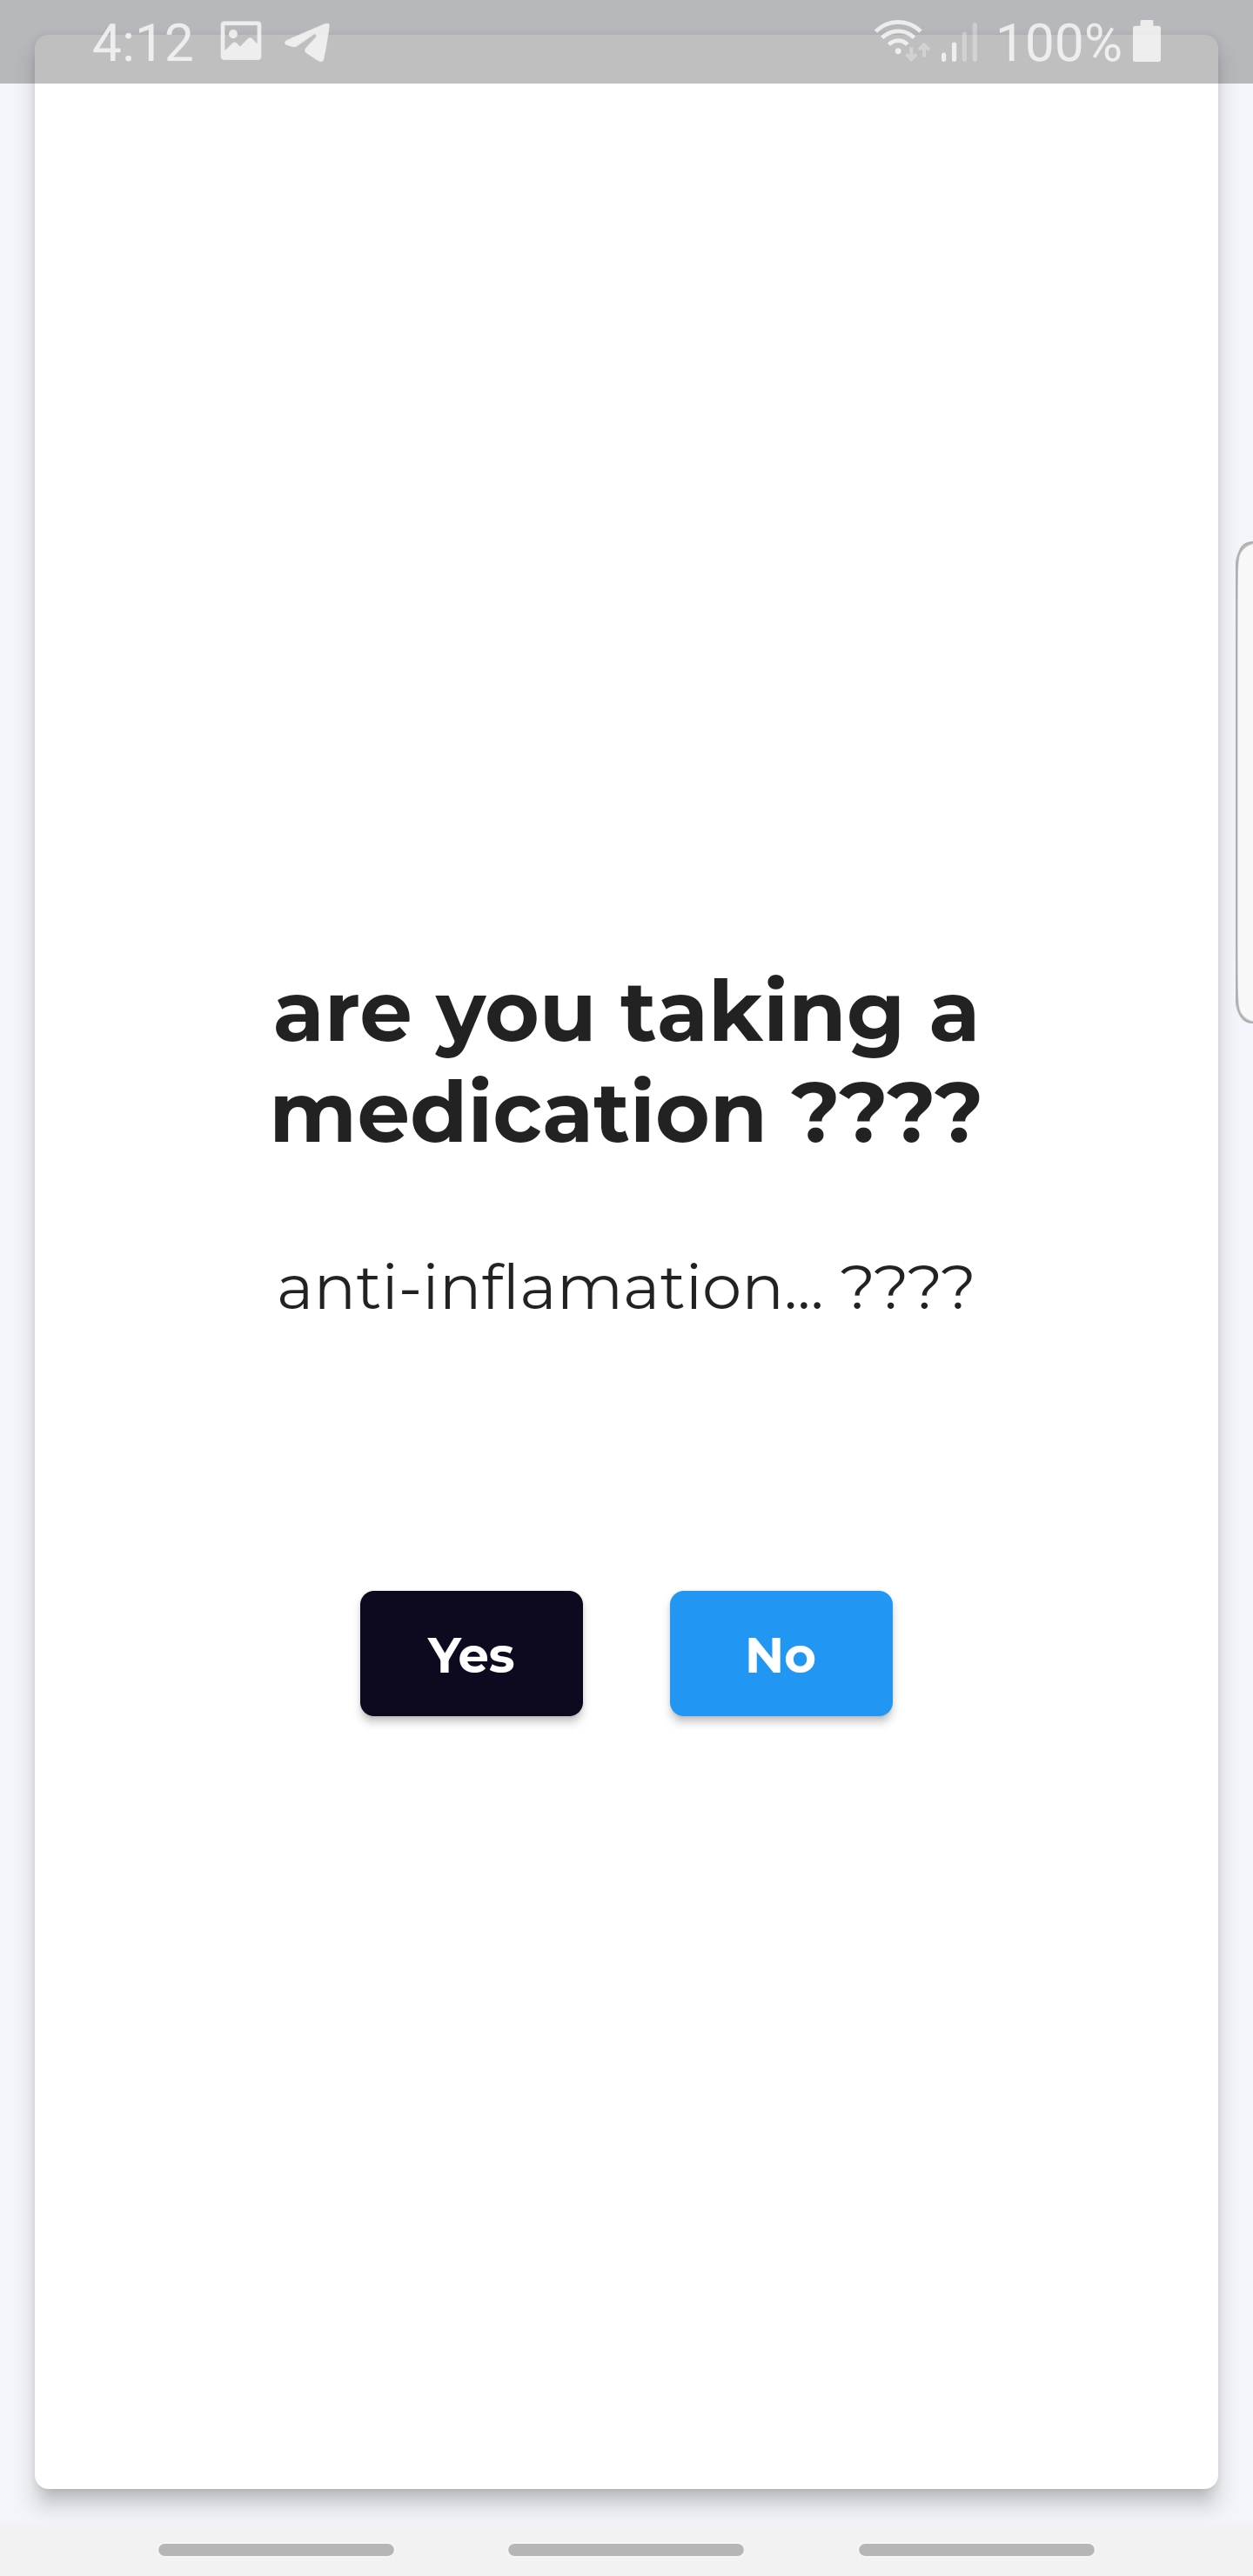
\includegraphics[width=1\linewidth]{images1/quess4.jpg}  
  %\caption{Put your sub-caption here}
  \label{fig:sub-fourth}
\end{subfigure}
\begin{subfigure}{.31\textwidth}
  \centering
  % include first image
  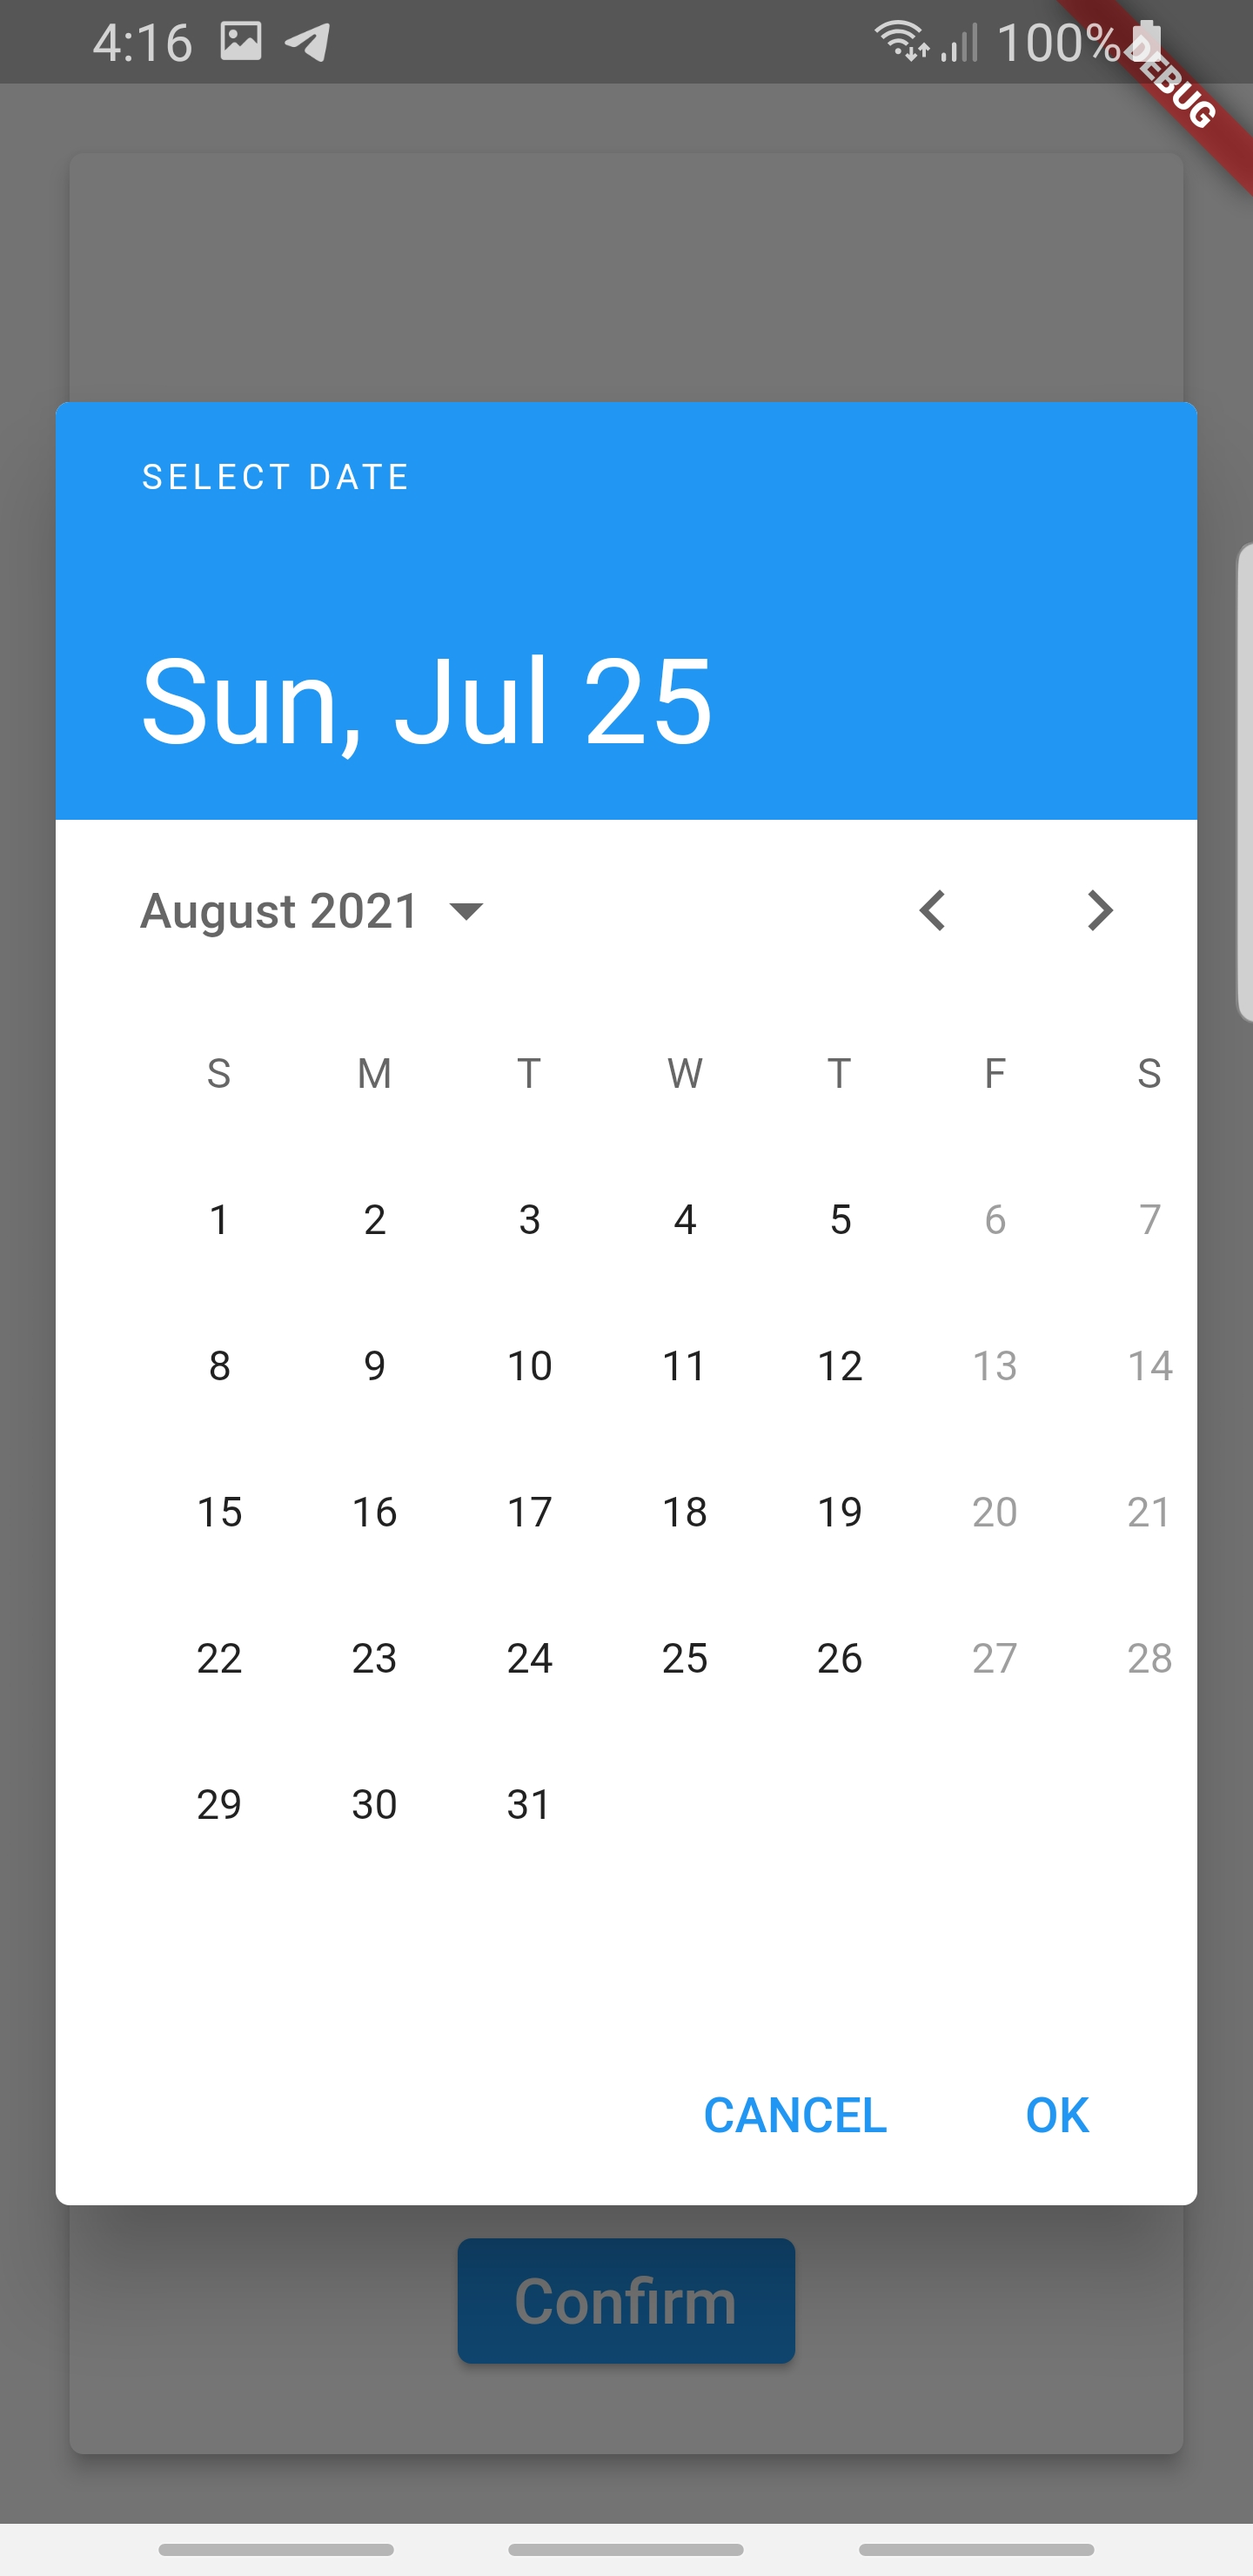
\includegraphics[width=1\linewidth]{images1/ques6.jpg}  
  %\caption{Put your sub-caption here}
  \label{fig:sub-first}
\end{subfigure}
\begin{subfigure}{.31\textwidth}
  \centering
  % include first image
  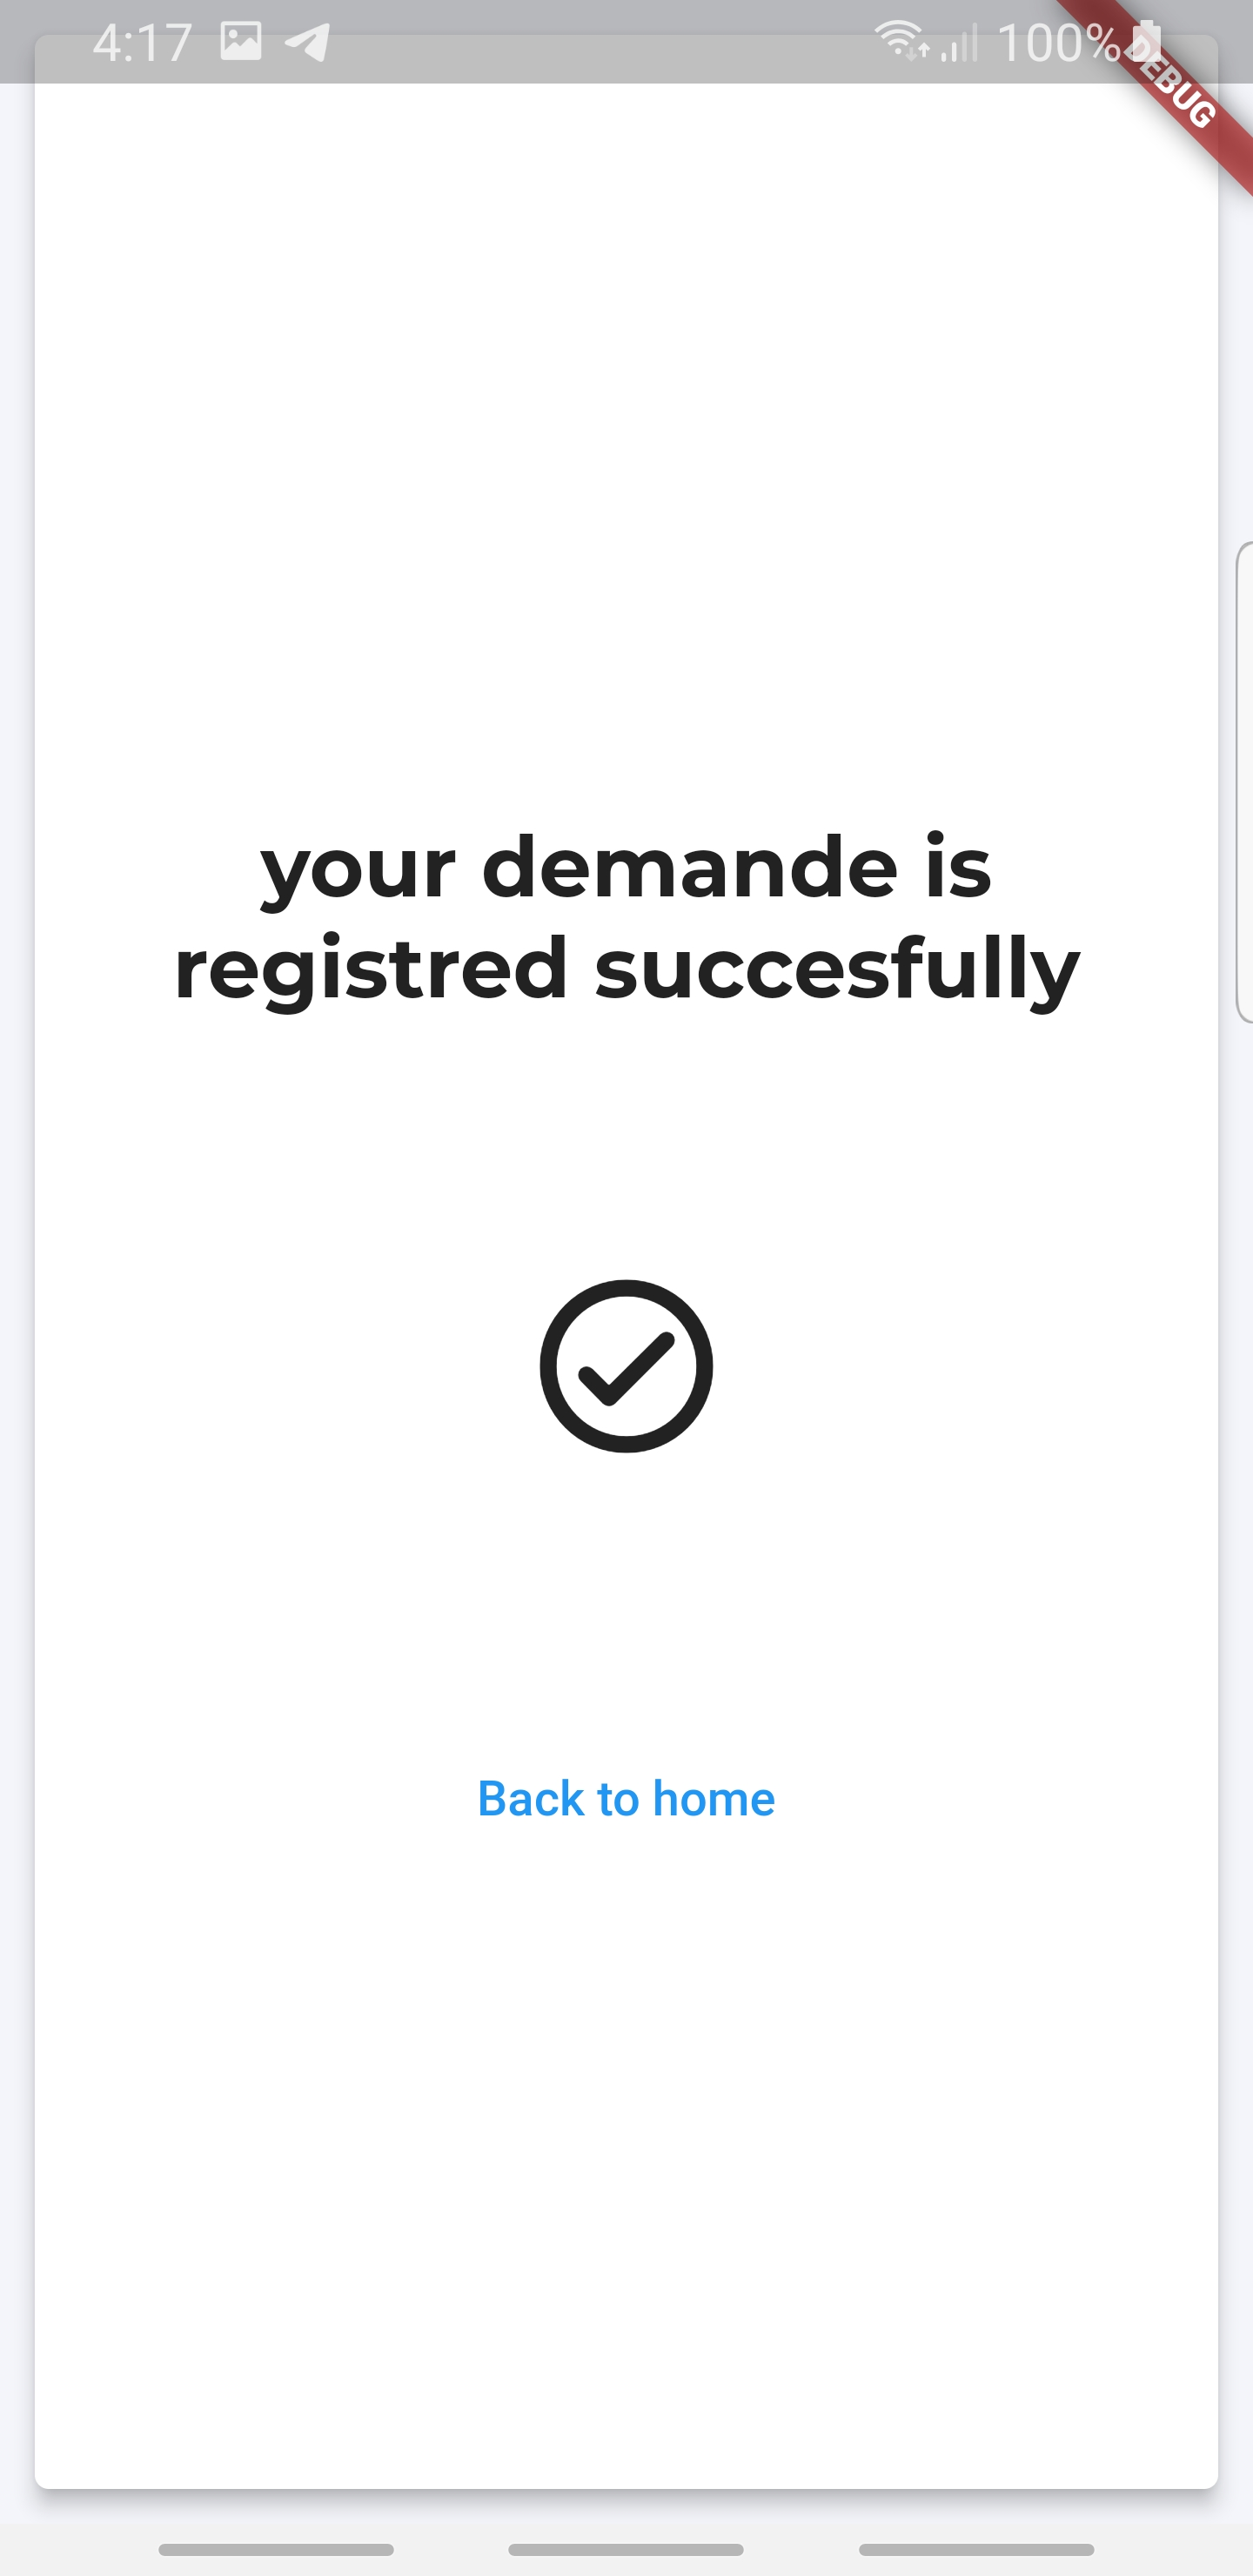
\includegraphics[width=1\linewidth]{images1/ques7.jpg}  
  %\caption{Put your sub-caption here}
  \label{fig:sub-first}
\end{subfigure}
\caption{Registration questions}
\label{fig:fig}
\end{figure}





\begin{figure}[H]
\centering

    \begin{subfigure}[b]{0.409\linewidth}
        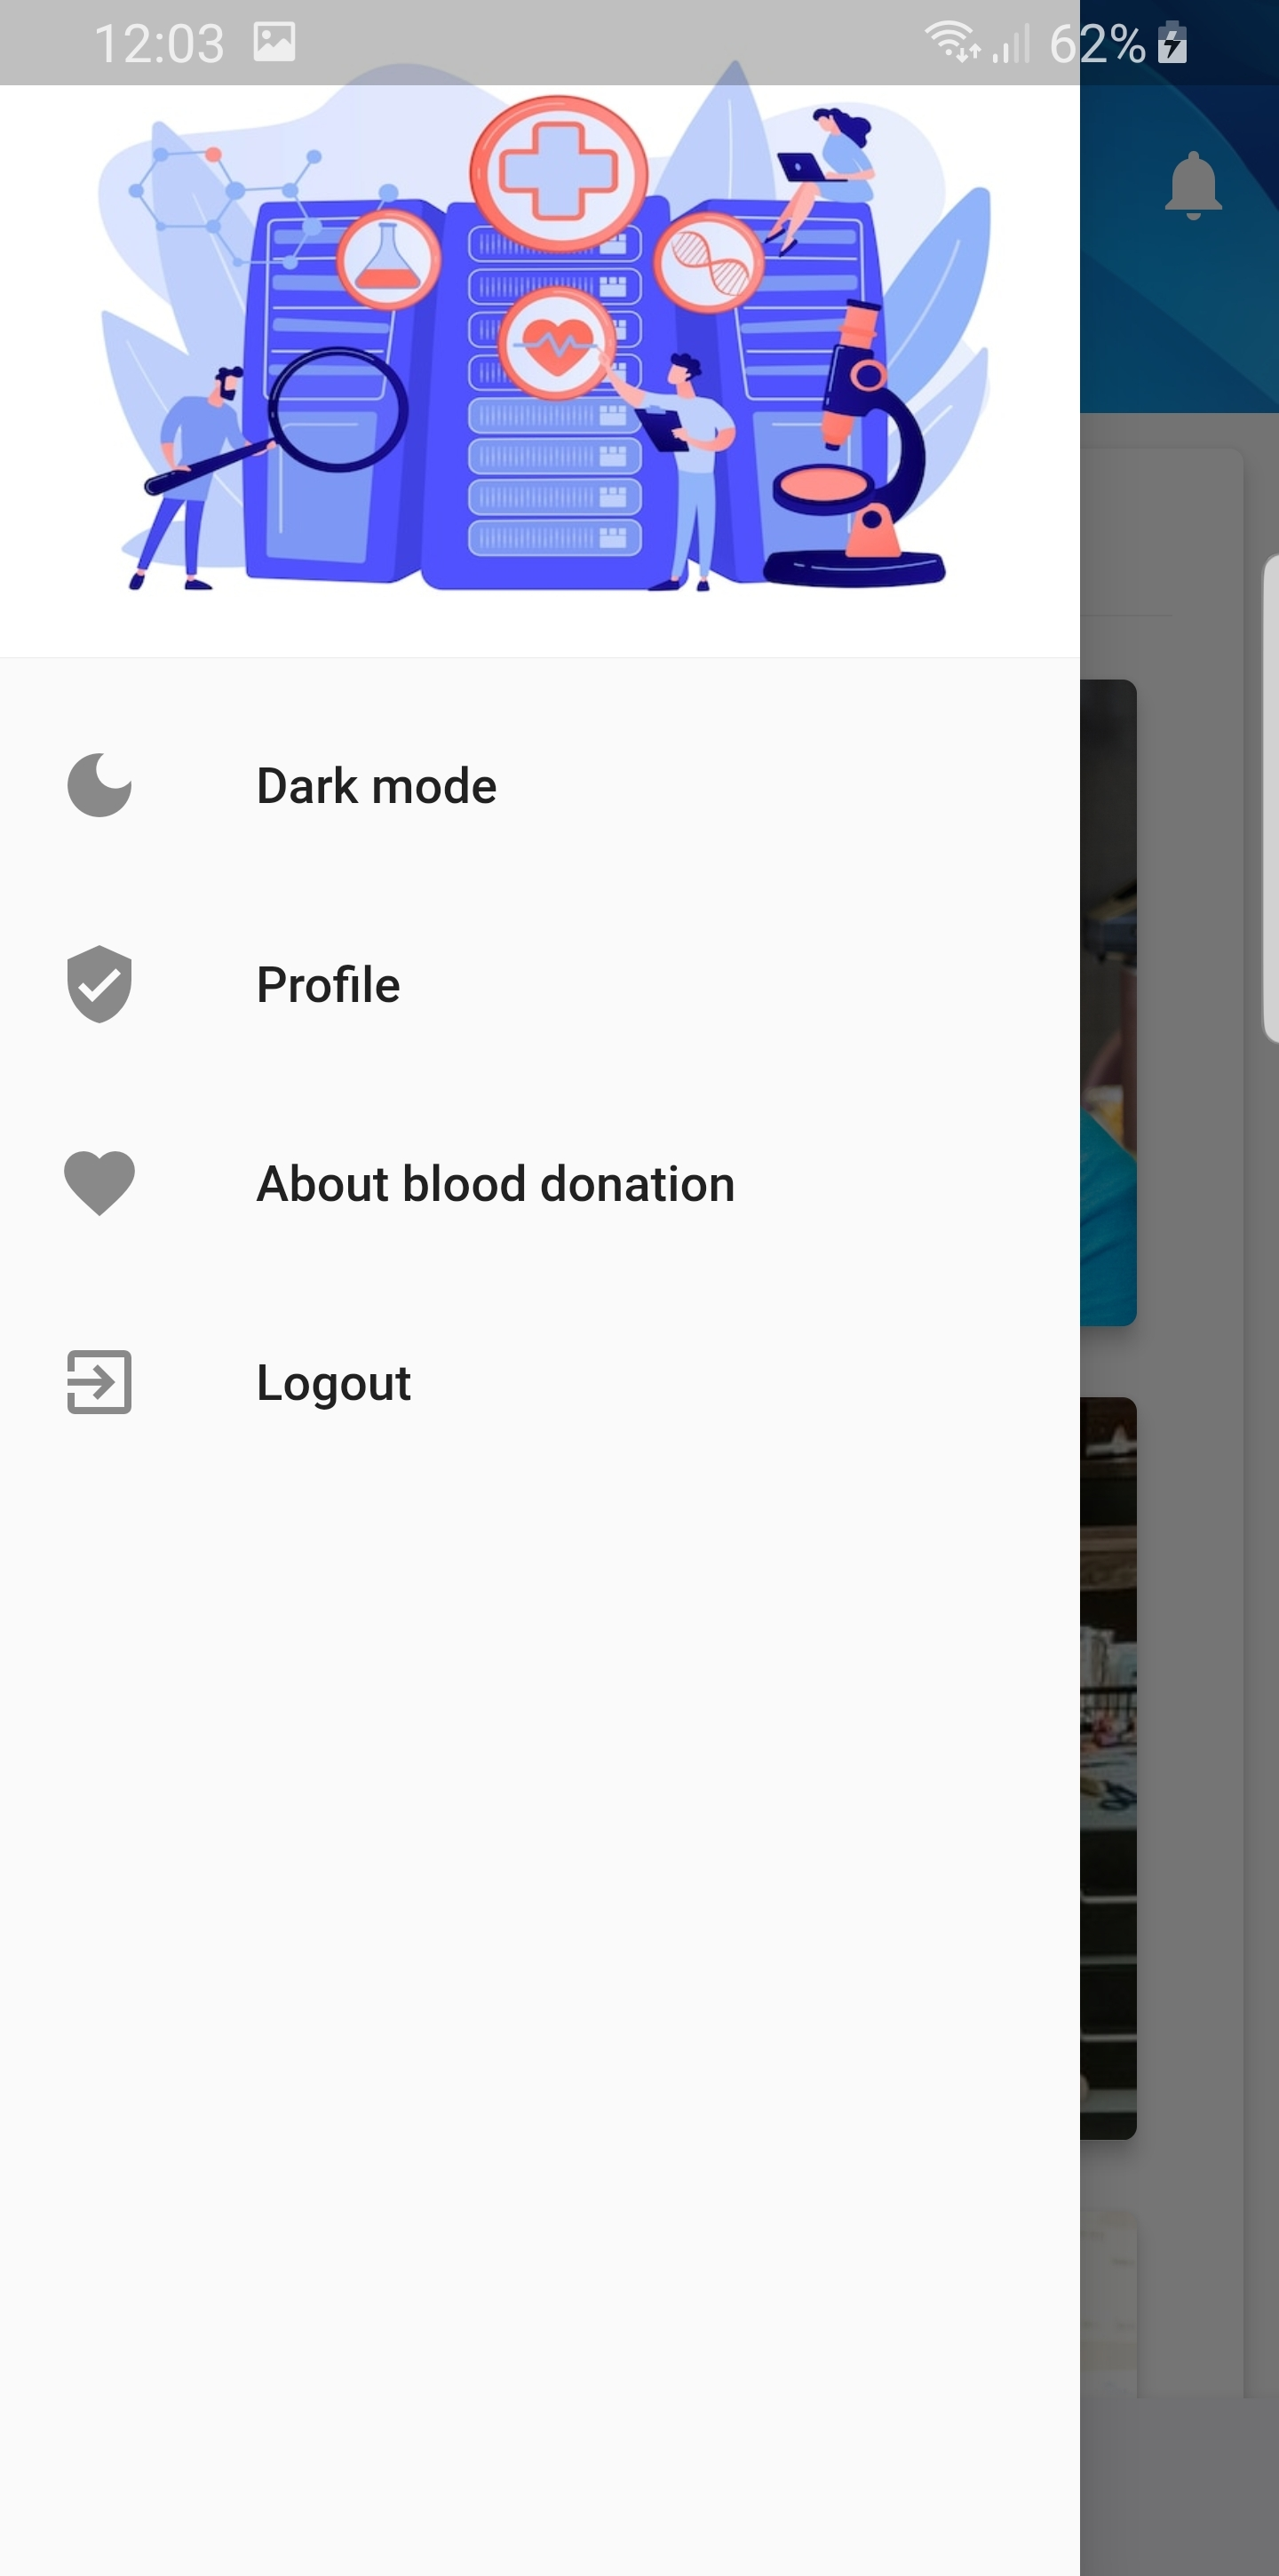
\includegraphics[width=\linewidth]{images1/sidebardonor.jpg}
    \caption{Donor side bar}
    \end{subfigure}
    \begin{subfigure}[b]{0.4\linewidth}
        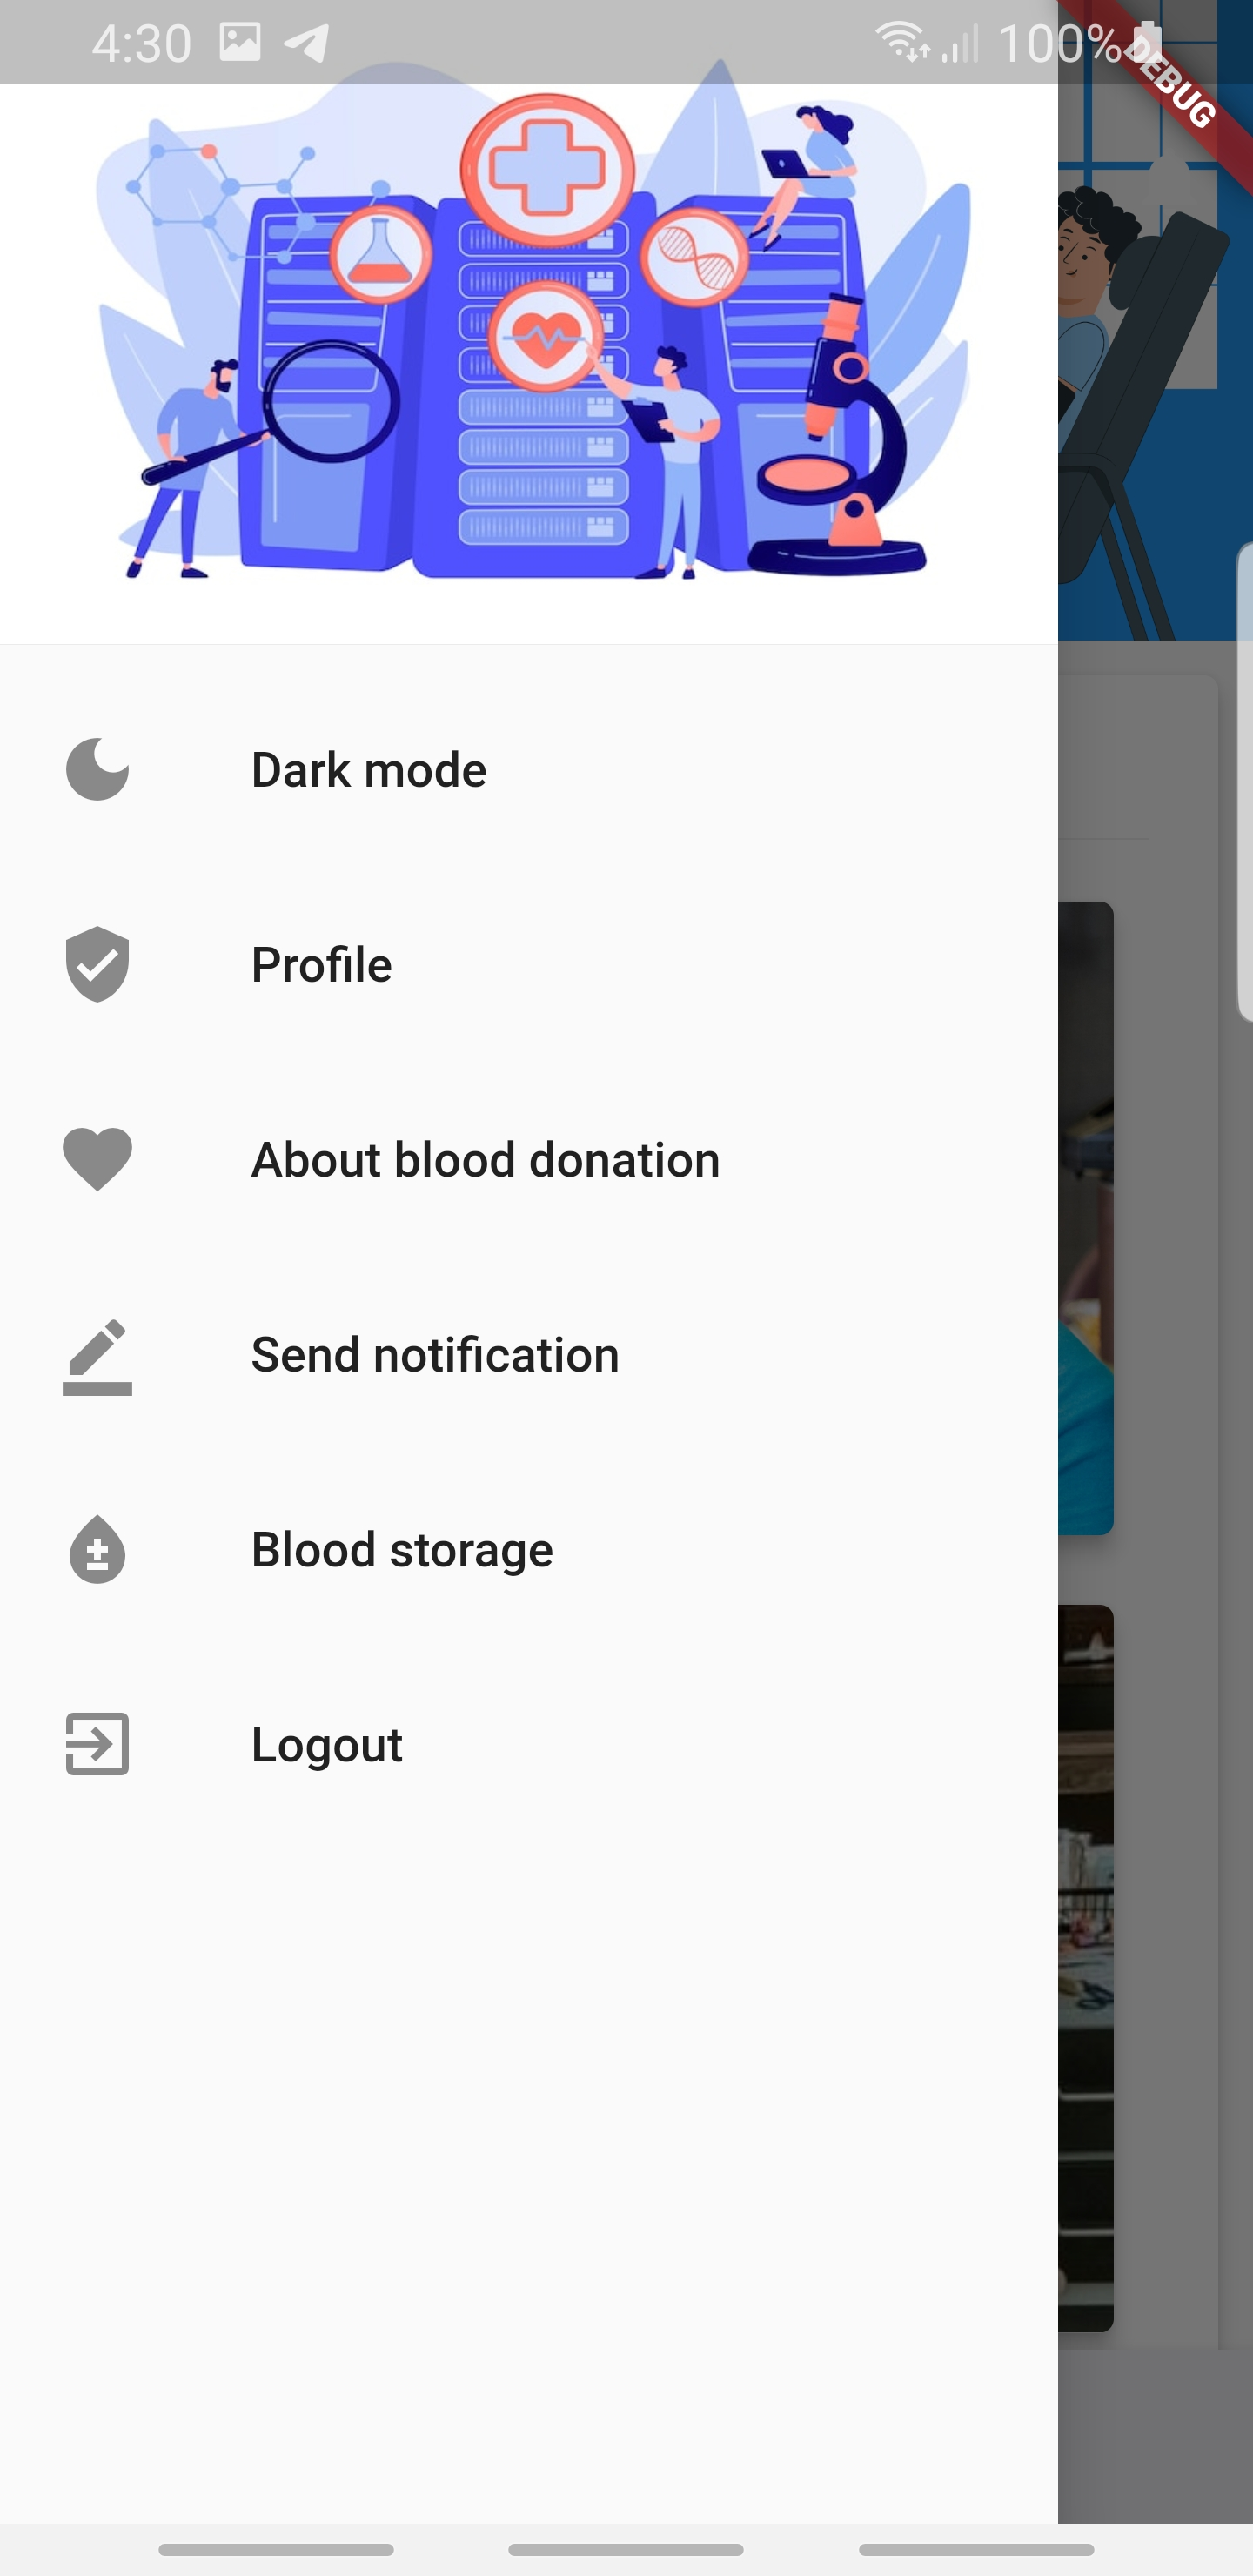
\includegraphics[width=\linewidth]{images1/sidebaradmin.jpg}
    \caption{Admin side bar}
    \end{subfigure}
\caption{Side bars}
\label{fig:distribution}
\end{figure}




\begin{figure}[H]
	\hspace{1cm}
	\begin {minipage}[t]{4cm}
	\centering
	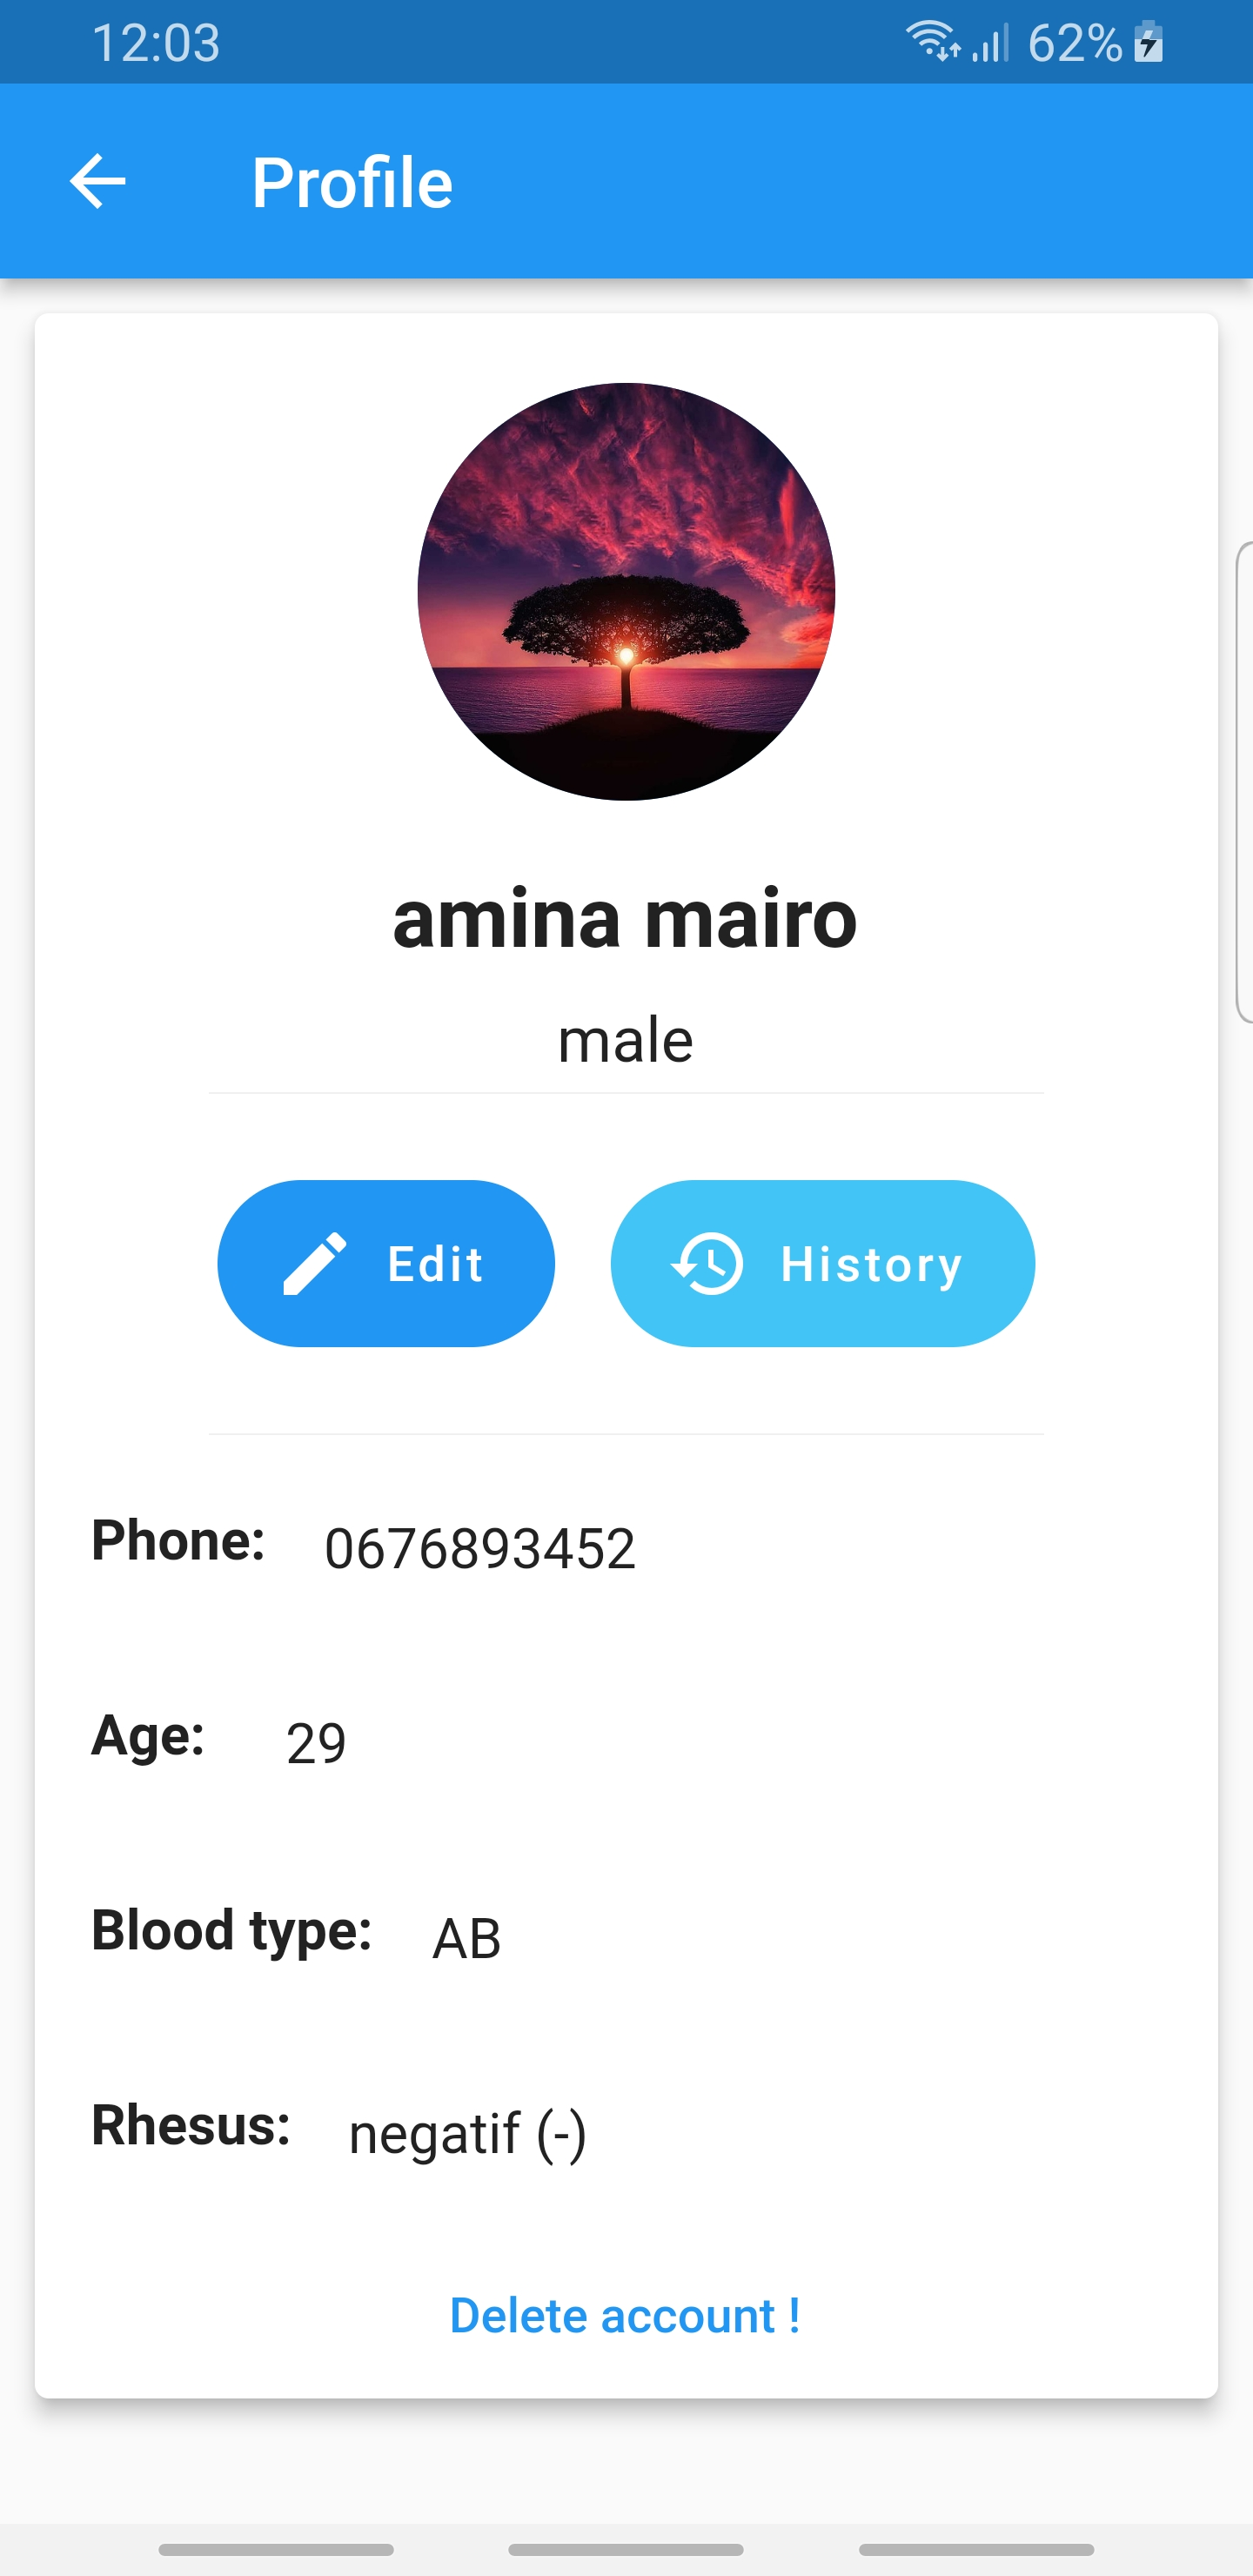
\includegraphics [ width =6 cm ]{images1/profile.jpg}
    \end {minipage}
	\hspace{2.5cm}
	\begin {minipage}[t]{4cm}
	\raggedright
	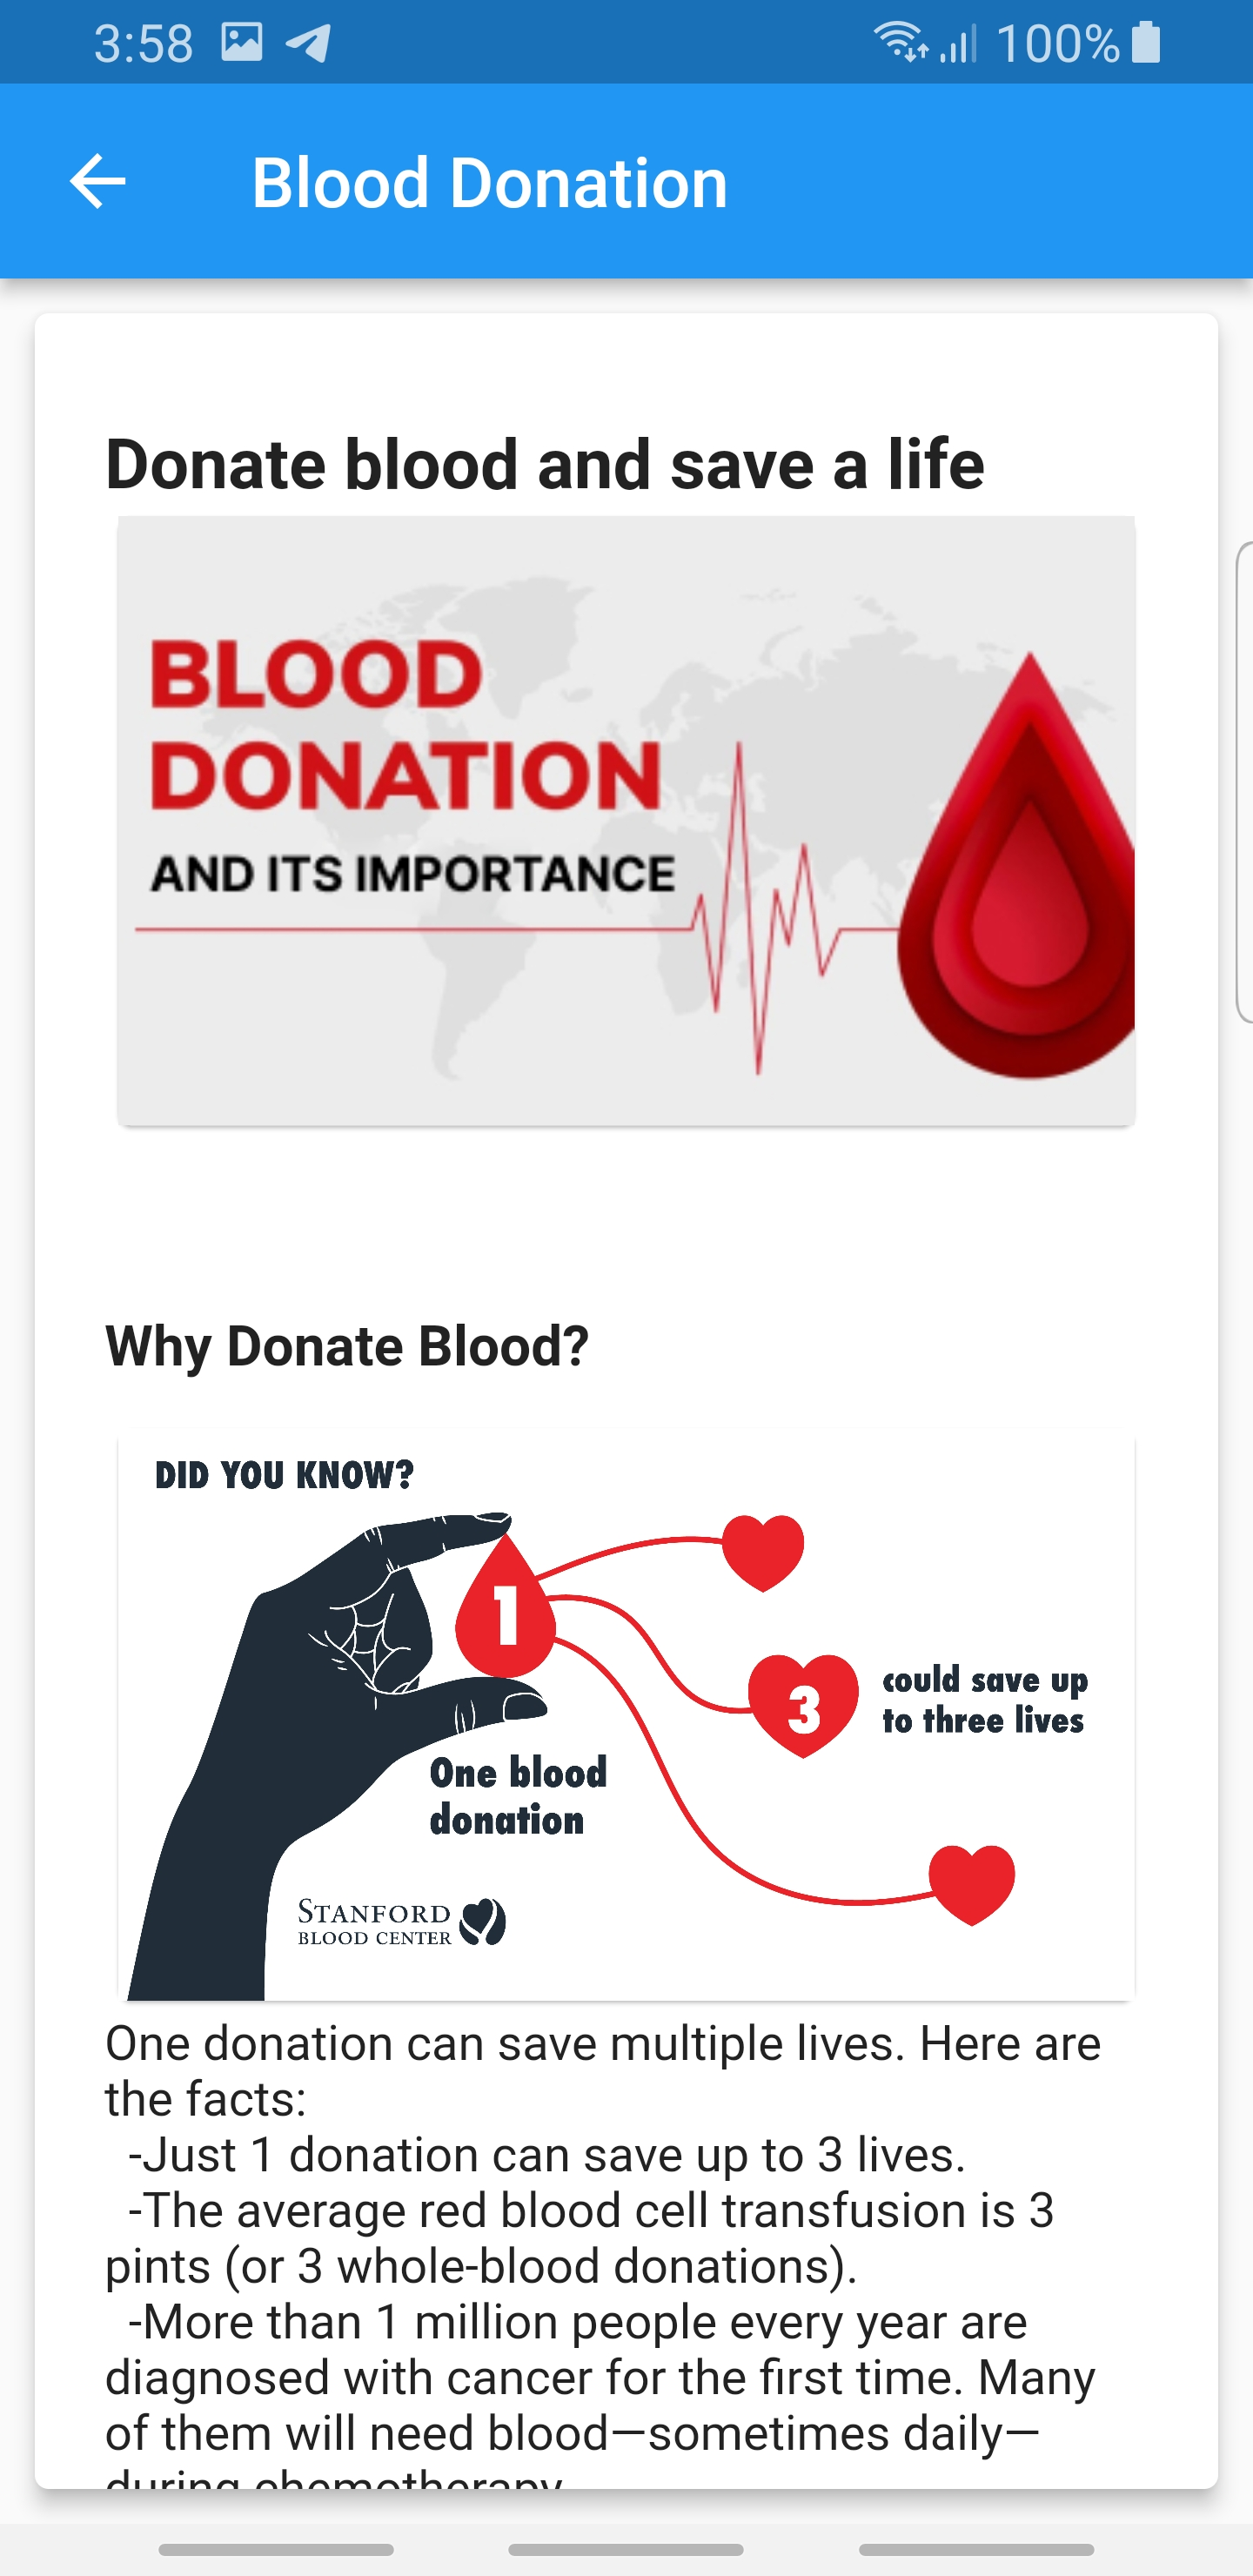
\includegraphics [ width =6 cm ]{images1/aboutbloodd.jpg}
	\end {minipage}
	\caption{Profile and Blood donation}
\end{figure}









\begin{figure}[H]
\begin{subfigure}{.31\textwidth}
  \centering
  % include third image
  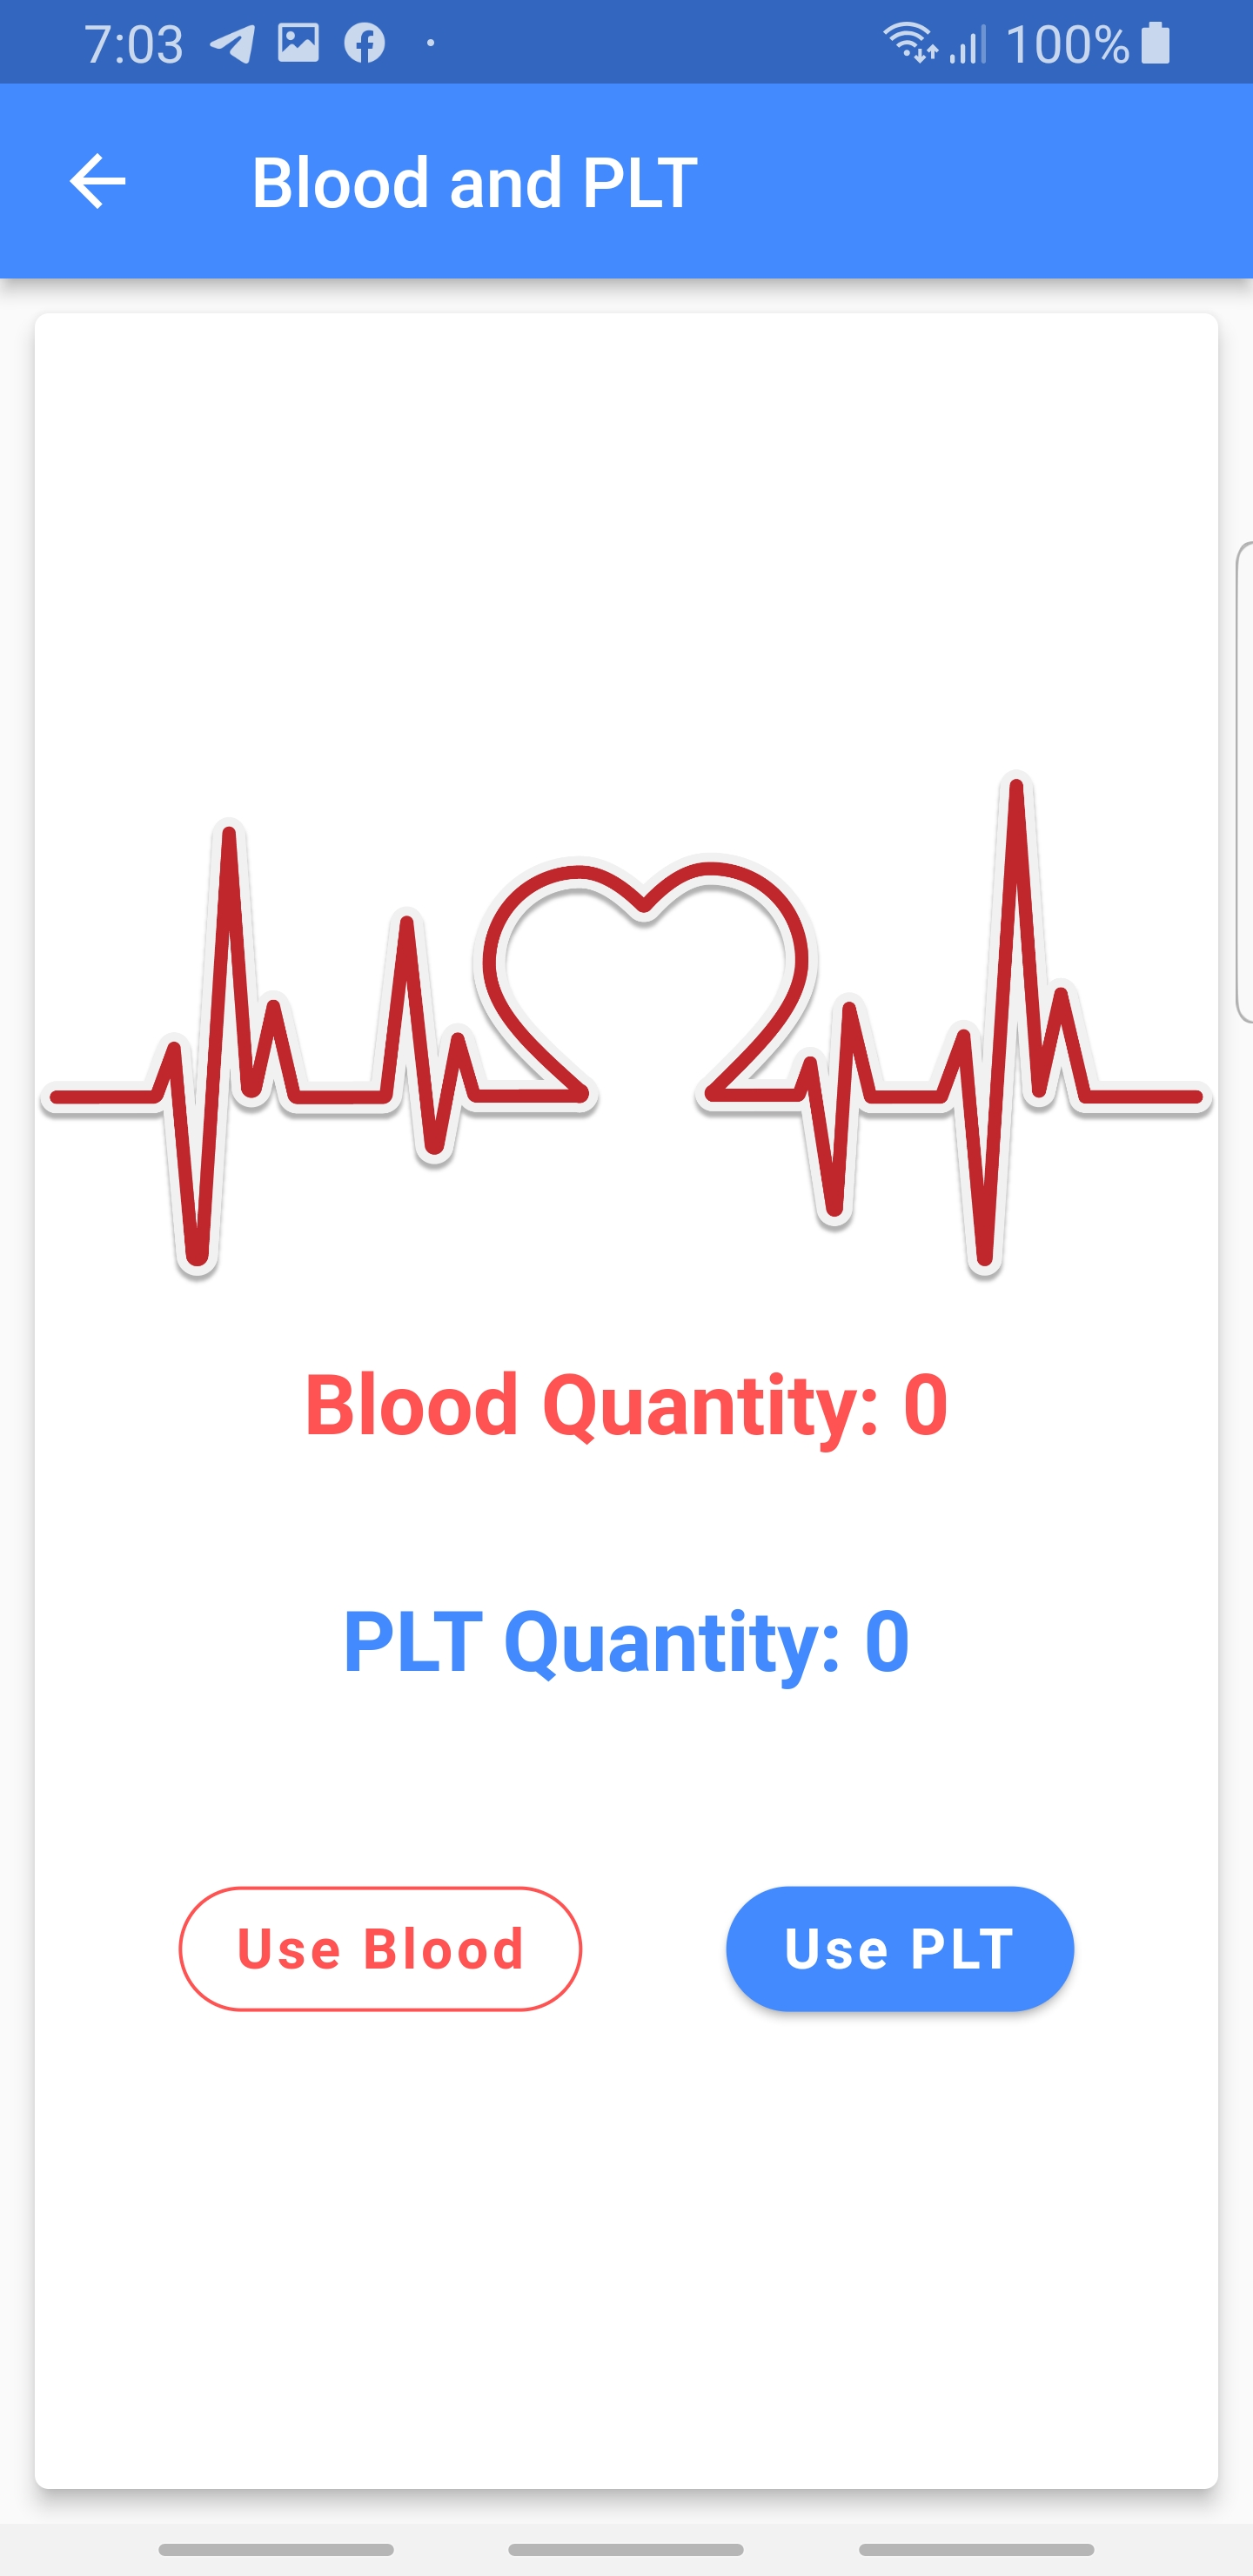
\includegraphics[width=1\linewidth]{images1/stocke.jpg} 
  %\caption{Put your sub-caption here}
  \label{fig:sub-third}
\end{subfigure}
\begin{subfigure}{.31\textwidth}
  \centering
  % include first image
  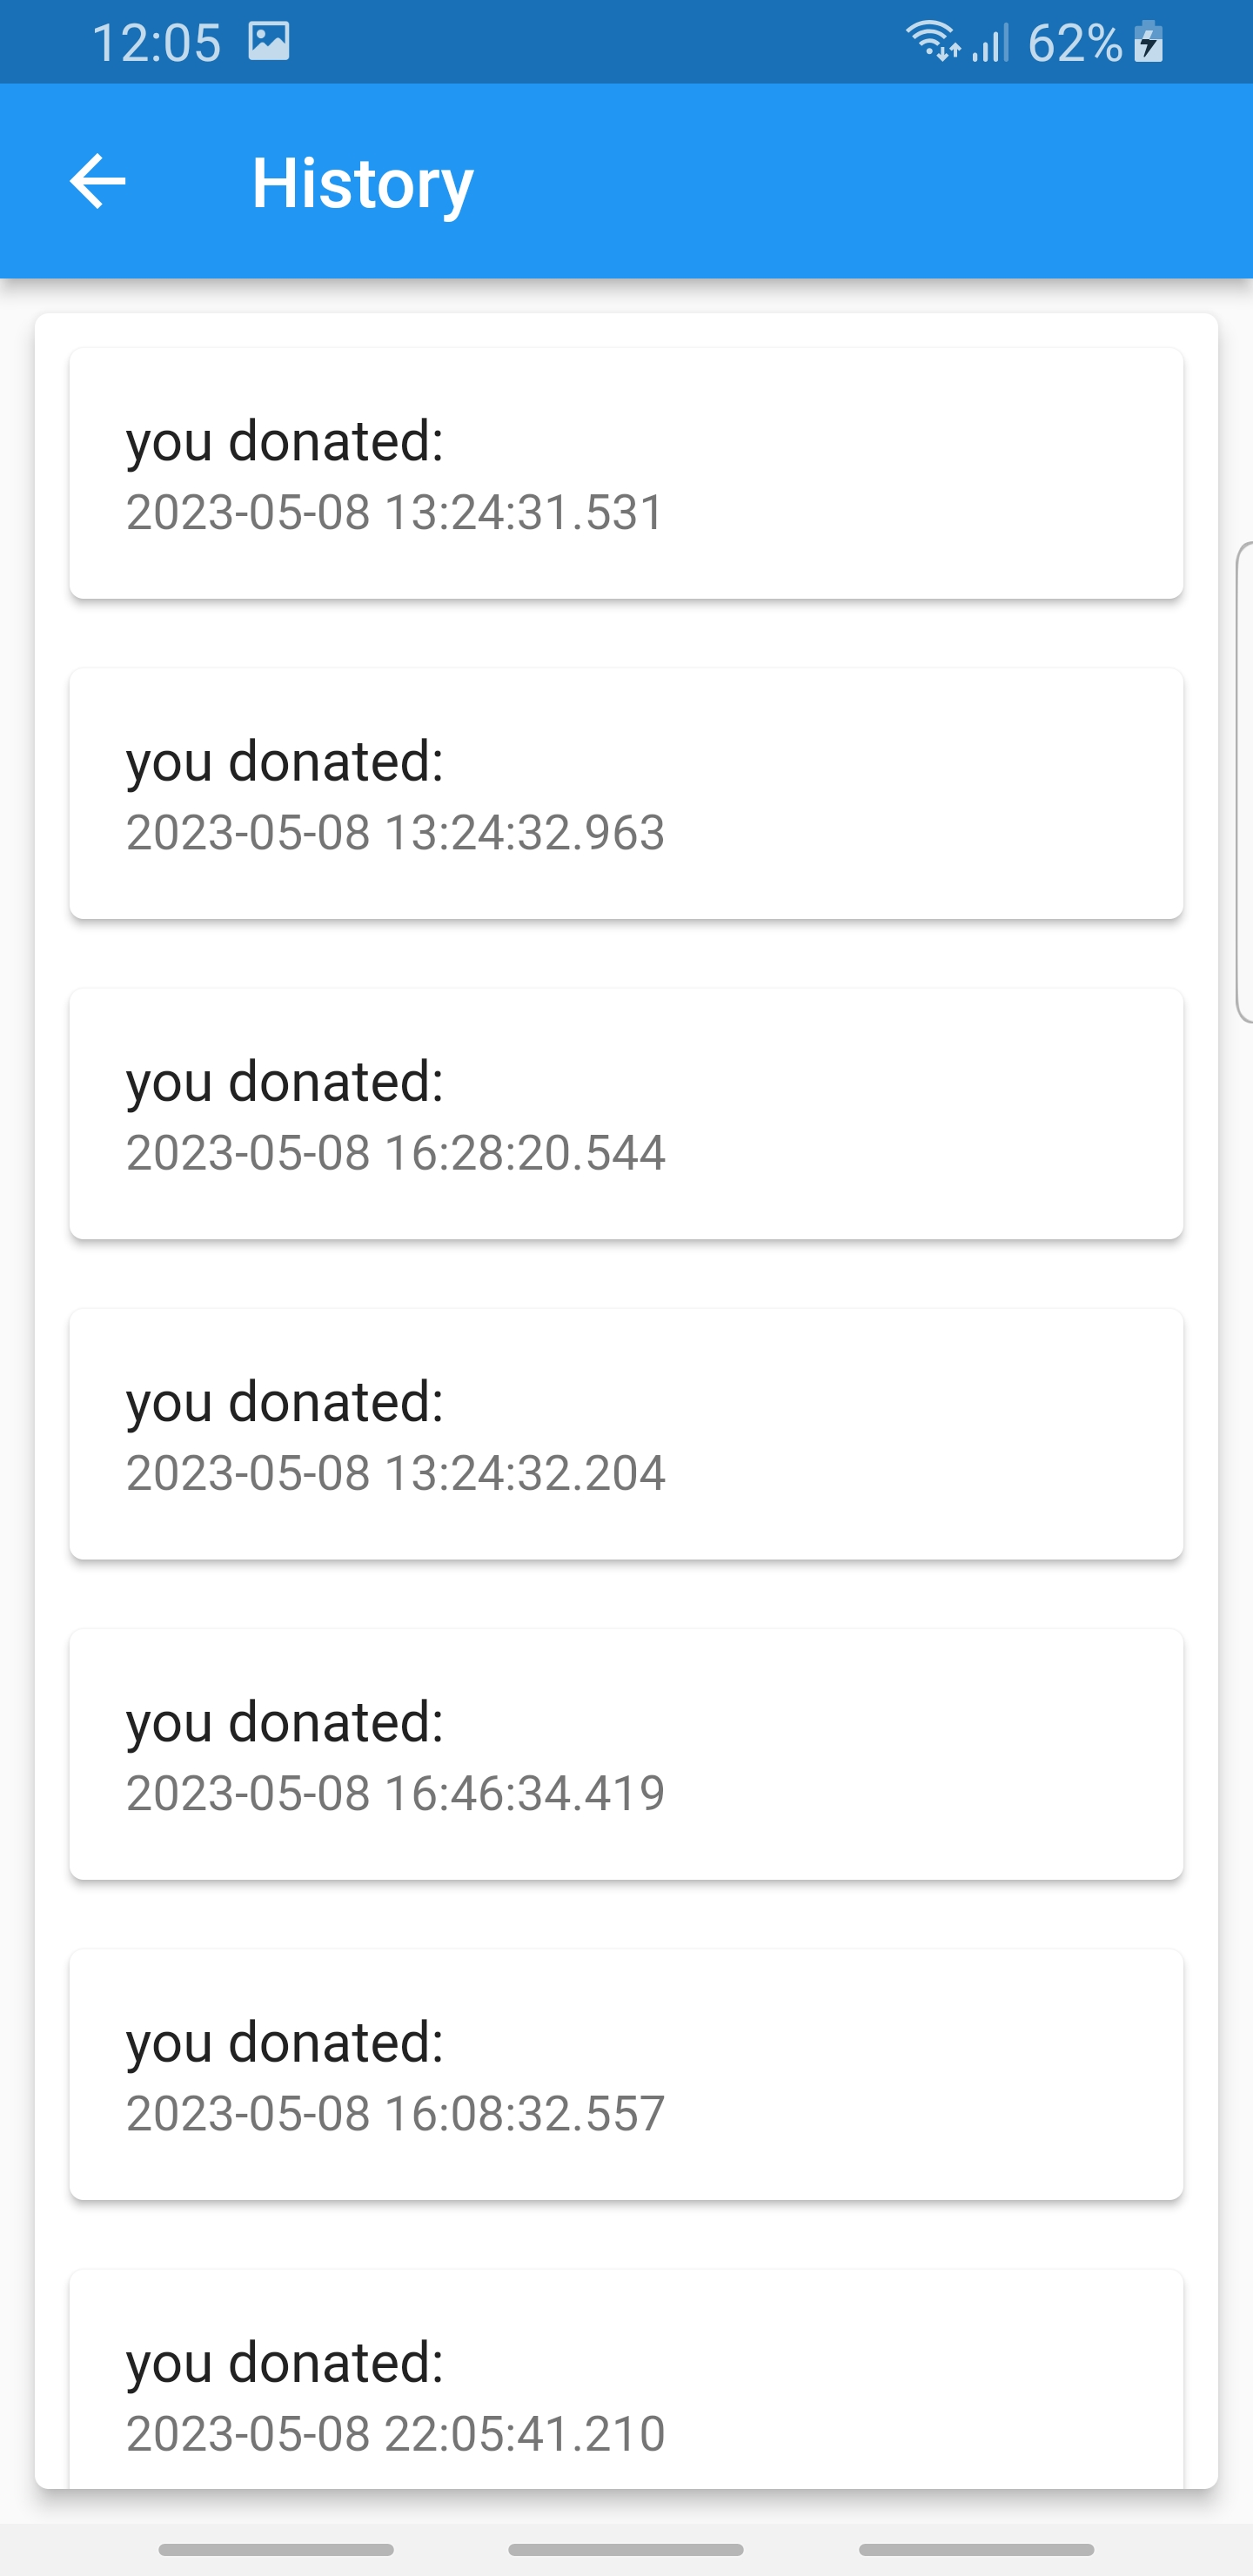
\includegraphics[width=1\linewidth]{images1/history.jpg} 
  %\caption{Put your sub-caption here}
  \label{fig:sub-first}
\end{subfigure}
\begin{subfigure}{.31\textwidth}
  \centering
  % include second image
  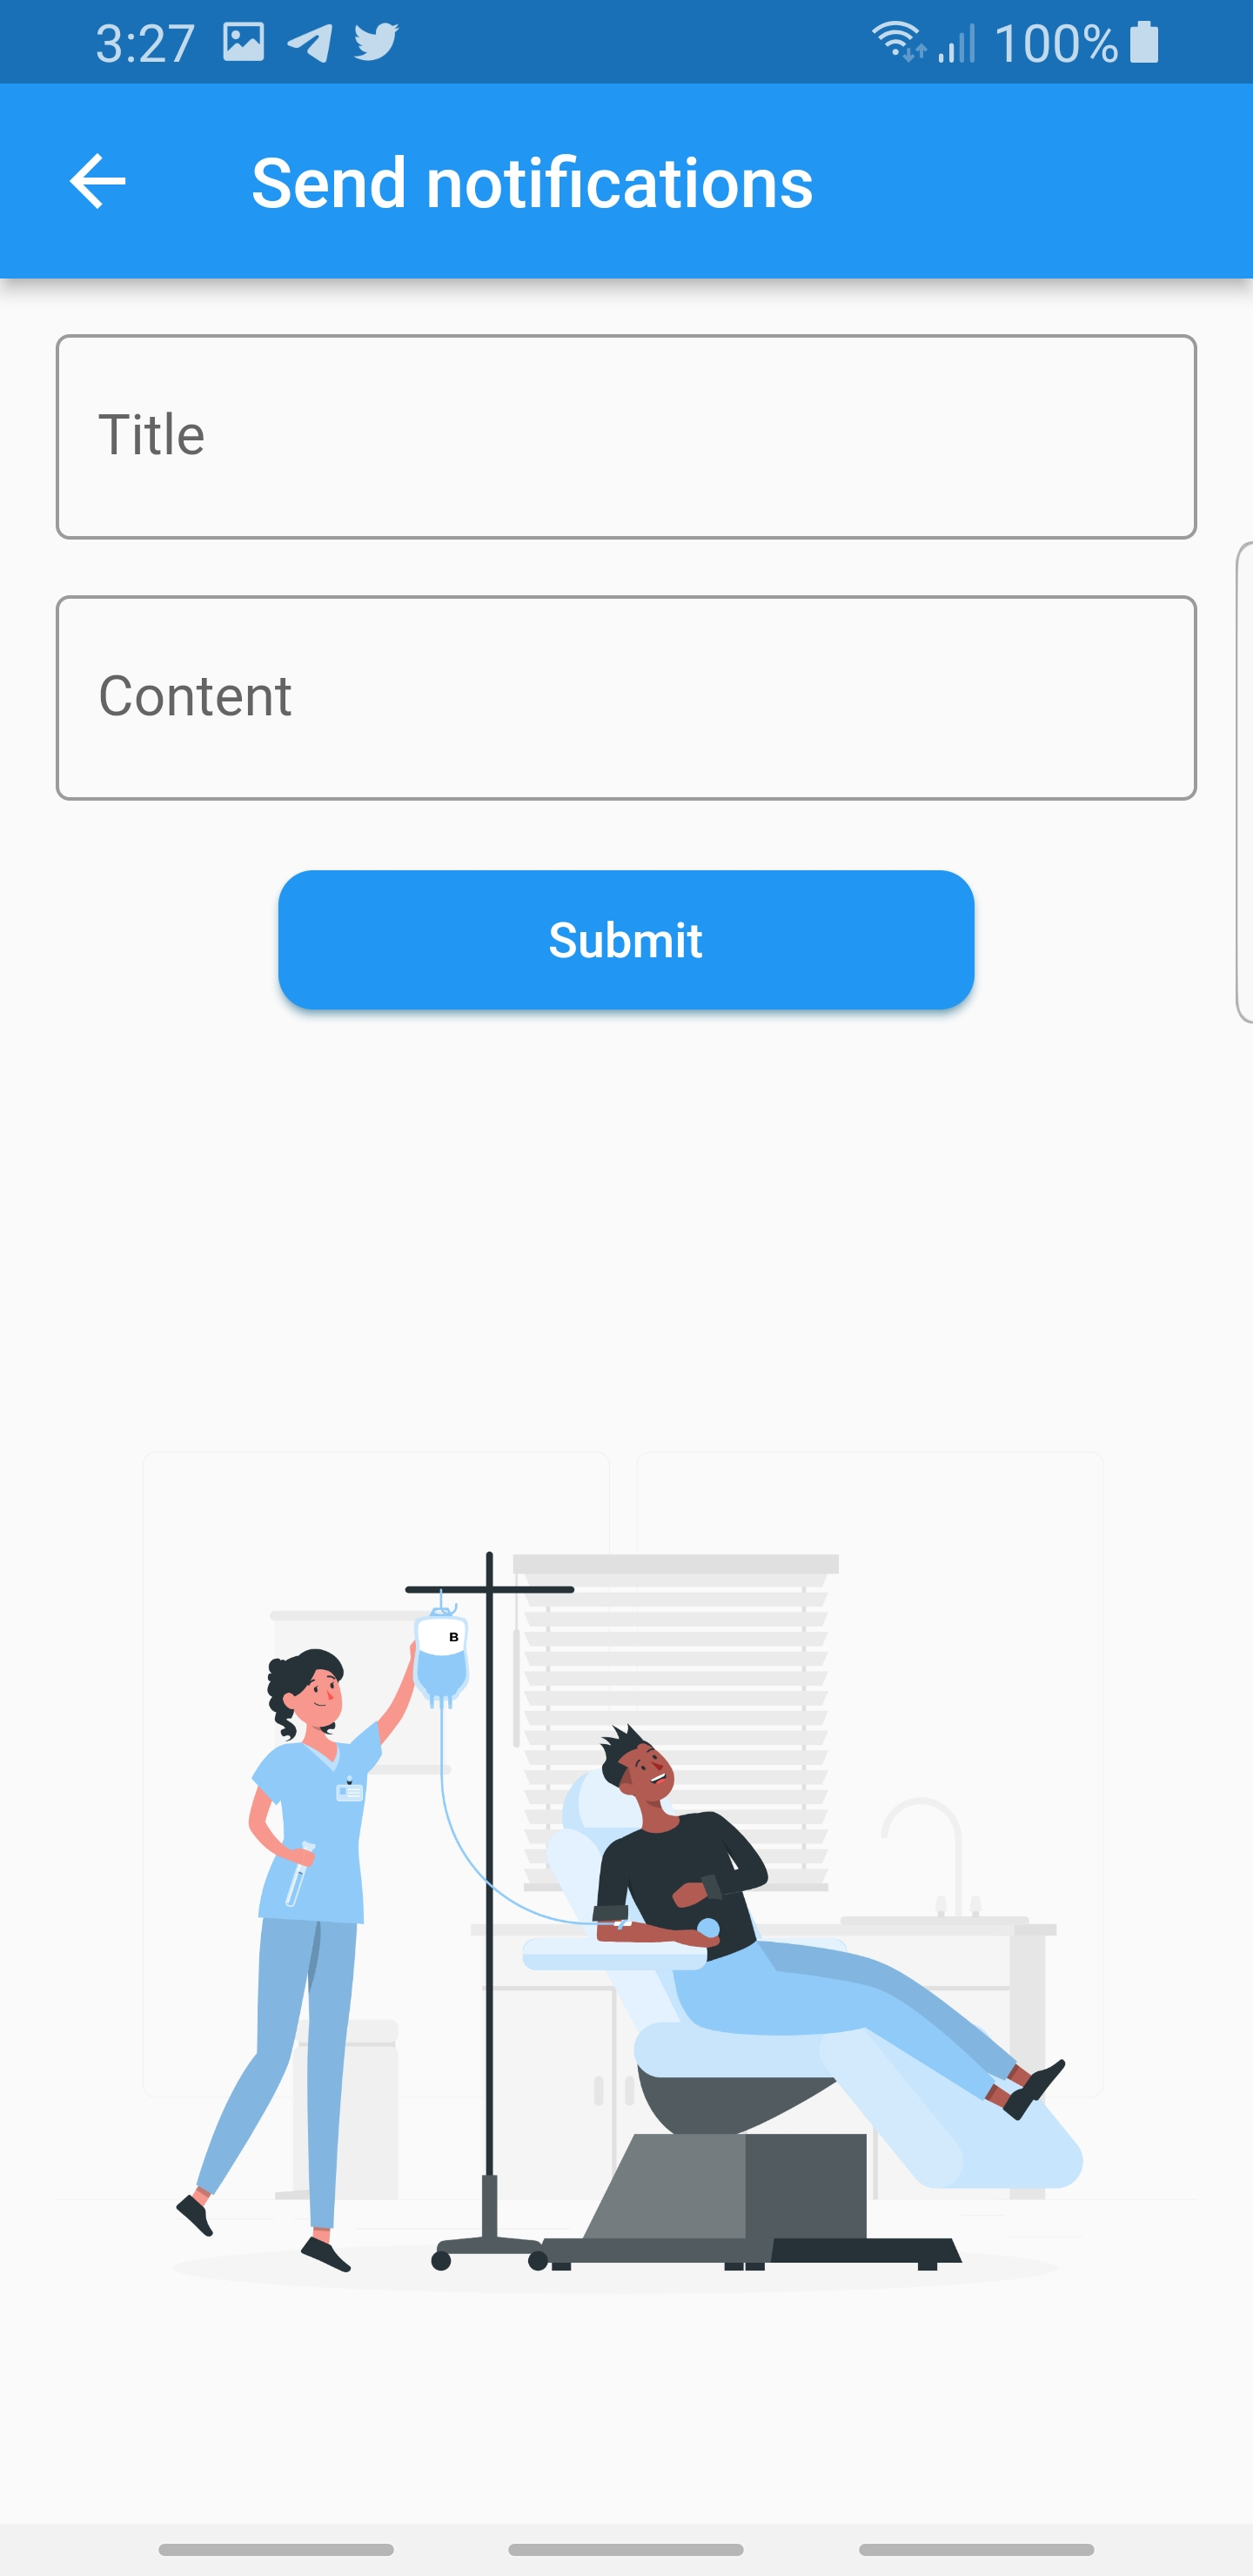
\includegraphics[width=1\linewidth]{images1/sendnotification.jpg}  
  %\caption{Put your sub-caption here}
  \label{fig:sub-second}
\end{subfigure}
%\newline


\caption{More functionalities}
\label{fig:fig}
\end{figure}





\section{Conclusion}
This chapter focused on the implementation process. First, we discussed the tools we used to develop the application, then we talked about the graphic chart and design, and finally, we showed some of the application interfaces with screenshots.




%\addcontentsline{toc}{chapter}{ Conclusion}



\chapter*{Conclusion}
\label{chp:conclusion}
\addcontentsline{toc}{chapter}{ Conclusion}


In conclusion, our blood donation app project aimed to provide a user-friendly platform for blood donors and donation centers. The development of the "Drop Angel" app allowed us to expand our knowledge and experience in mobile app development while also contributing to a noble cause. Throughout the project, we faced challenges and limitations, such as the need for better documentation and more time for testing and implementing additional features.

However, we were able to successfully complete the project and believe that the app has the potential to make a positive impact on blood donation efforts. We hope that our project serves as a starting point for further development and innovation in the field of blood donation apps.


During our research, we found that there was a need for a blood donation app with a simple and intuitive design, which could be easily used by donors and blood donation centers alike. Our "Drop Angel" app aims to meet this need and facilitate the donation process.

Looking to the future, we plan to further enhance our app's functionality by adding features such as a rewards system to incentivize donors, as well as integrating with other healthcare apps for a more comprehensive approach to healthcare.

%\appendix

%\chapter{My Appendix}
%\lipsum[1-3]

\bibliographystyle{ieeetr}
\bibliography{thesis}



%\input{zz-korean-summary.tex}

\end{document}

